\chapter{ASR system - Improvements \& sensitivities}
\label{chapter:model_scenarios}
In the north of Ghana farmers are in search of sources to increase the water availability during dry season. This chapter investigates to what extent an Aquifer Storage and Recovery (ASR) system, and the potential improvements of the system, can provide solutions. The options are explored by the use of a hypothetical ASR system. The synthetic model is adapted to potential northern Ghana conditions by the use of the geohydrological parameters found in aquifer test data analysis (Chapter \ref{section:fieldwork_conclusions}). \\
In Section \ref{section:test_problem_def}, the applied soil scenarios are presented and a base model ASR system simulation is defined. Moreover, the types of ASR system improvements, sensitivities and test criteria are included in this section. The year-round performances of the synthetic ASR system are explained in Section \ref{section:Base_model_perf}. Section \ref{section:ASR_upscaling} contains the results of three types of ASR system improvements; (a) the extension of daily pumping time, (b) the enlargement of the borehole cross-sectional dimension and (c) the reduction of the well skin resistance. In Section \ref{section:sens_analysis}, the ASR systems interaction with nature is explored by a sensitivity analysis on; (a) the degradation of well depth by clogging; (b) the shortening of the wet season inundation time-span and (c) the reduction of the wet season inundation levels. The relations between soil conditions and the different ASR system improvements and sensitivities are presented in Section \ref{section:dim_fac}. The Chapter ends with a discussion on the obtained results, Section \ref{section:Upscaling_conclusions}. 
%
%% increased water quantities
%
% 
% This chapter explores the impact of ASR system modifications.   contribute. the contribution of an ASR system can be on  spresents the results of potential improvements of a synthetic ASR system in northern Ghana. A synthetic problem is defined (Section \ref{base_model_def}) as reference.   First, Second, 
%
%The scenarios are based on the defined bandwidth of geohydrological parameter values found in fieldwork data analysis. 
%
% quantities of water during dry season. 
%
%
%e general aim of research is pointed at the provision of larger water quantities during northern Ghana's dry seasons. The research investigates to what extent Aquifer Storage and Recovery systems (ASR-systems) can contribute to water availability. The water is in the essence used for local small-scale agriculture. \\
%%
%A single test problem is selected to explore and access the capabilities in ASR-system upscaling. The test problem consists of a single layer aquifer which is partially penetrated by a well. In accordance with \citet{HoughtonMifflin2016}, upscaling can be defined as \emph{"The raise to an higher level; an upgrade"}. Free interpretation learn, multiple directions of upscaling are applicable. The single test problem is exposed to three types of ASR-system upscaling; (a) upscaling in dry season daily pumping time, (b) upscaling the borehole cross-sectional dimension and (c) upscaling by ASR-system cleaning. \\
%%
%%The hypothetical northern Ghana test problem will be outlined first. It concerns both the natural (Section \ref{section:test_problem_def}) as well as the model-based description (Section \ref{section:MODFLOW_const}). As a follow-up, the unimproved (base) model performance is described (Section \ref{section:Base_model_perf}). The section can be used as reference material for the different types of system upscaling (Section \ref{section:ASR_upscaling}). The chapter concludes with a discussion on the (ASR-system upscaling) results obtained (Section \ref{section:Upscaling_conclusions}). 
%
%How and to what extent can improvements of an ASR system increase the water supply to northern Ghana smallholder framers, while sustainability is maintained?
%
%For northern Ghana smallholder farmers this question is key, but the answer to it is rather challenging. The terms 'how' (types of improvement) and 'to what extent' (limit of sustainability) need further specifications. In order to judge the improvements of the ASR system, comparison material is required. A northern Ghana synthetic base model is defined as reference (Section \ref{section:test_problem_def}). The outcomes of the (improved) system simulations are elaborated in Chapter \ref{chapter:model_scenarios}.
%
%
%%The performance of an ASR system is dependent on the physical properties of its surroundings \citep{Bakker2010}. Geological conditions are heterogeneous in northern Ghana. Subsurface characteristics vary at short mutual distances \citep{Owusu2017}. In this research, local geohydrological conditions were gathered through site-specific fieldwork. Pumping tests were performed at multiple locations in northern Ghana. The study sites are presented in Section \ref{section:research_locations}. The raw results of these measurement can be found in Appendix \ref{chapter:fieldworkresults}. In Section \ref{section:TS}, the pumping test data is analysed. The drawn conclusions on the site visits and data analysis are described in Section \ref{section:fieldwork_conclusions}. The chapter concluded with the derivation of locally applicable values for $T$ and $S$. The geohydrological parameters are the input for the study on impacts of ASR system improvements in northern Ghana. 

%\section{Methods - ASR system improvements}
\section{Methods - ASR system simulation}
\label{section:test_problem_def}
In this methodology part a synthetic ASR system is presented to explore and access the system (improved) performances. The applied representations of (northern Ghana) natural conditions are defined. The section contains information on: soil scenarios; the ASR system base model (reference); the types of ASR system improvement/sensitivity and the research test criteria. The methods are implemented in the subsequent parts of this Chapter (Section \ref{section:Base_model_perf} - \ref{section:Upscaling_conclusions}). Additional information on the modelling environment (MODFLOW) is included in the Appendices \ref{chapter:Extense_Modflow_model} - \ref{MODFLOW_radial}. 

%The synthesis simulation of northern Ghana natural conditions are represented in a simplified synthetic model. The model representation of nature is defined in this part of the research methodology. of the system in northern Ghana conditions
%General aim of research is pointed at the provision of larger water quantities during northern Ghana's dry seasons. The research investigates to what extent Aquifer Storage and Recovery systems (ASR-systems) can contribute to water availability. The water is in the essence used for local small-scale agriculture. \\
%
%in ASR-system improvements upscaling. The test problem consists of a single layer aquifer which is partially penetrated by a well. In accordance with \citet{HoughtonMifflin2016}, upscaling can be defined as \emph{"The raise to an higher level; an upgrade"}. Free interpretation learn, multiple directions of upscaling are applicable. The single test problem is exposed to three types of ASR-system upscaling; (1) upscaling in dry season daily pumping time, (2) upscaling the borehole cross-sectional dimension and (3) upscaling by ASR-system cleaning. \\
%
%The hypothetical northern Ghana test problem will be outlined first. It concerns both the natural (Section \ref{section:test_problem_def}) as well as the model-based description (Section \ref{section:MODFLOW_const}). As a follow-up, the unimproved (base) model performance is described (Section \ref{section:Base_model_perf}). The section can be used as reference material for the different types of system upscaling (Section \ref{section:ASR_upscaling}). The chapter concludes with a discussion on the (ASR-system upscaling) results obtained (Section \ref{section:Upscaling_conclusions}).
 
\subsection{Soil scenarios}
\label{subsection:soil_sc_def}
The northern Ghana geohydrological conditions are potentially represented by the results from the aquifer test data analysis in Chapter \ref{chapter:Fieldwork_data_analysis}. The derived parameter bandwidth (Figure \ref{fig:Parameter_bandwidth}) is used to adapt the synthetic ASR system to locally applicable conditions. Transmissivity ($T$) values in the scope of 1 - 100 (m$^2$/d) and storativity ($S$) values between 1e-3 - 1e-2 (-) are taken into account by the definition of five soil scenarios. An overview of the research soil scenarios is presented in Figure \ref{fig:Schematic_base_model}.

\subsection{ASR system - Synthetic base model definition (reference)} 
\label{base_model_def}
The research is provided with an ASR system base model. Unsurprisingly, the base model accommodates basic conditions. The applied conditions are based on the northern Ghana study site inspections and the gathered borehole log sheets (Appendix \ref{chapter:Borehole_logsheets}). The simplified model represents a hypothetical 'standard' ASR system, potentially applicable in northern Ghana. The base model is a reference, a starting point to which the impact of system improvements can be compared. The distinctive modelled components (e.g. subsurface, well characteristics and simulation time frame) are one-by-one described. The overall representation of the base model (with the inclusion of the soil scenarios) is presented in Figure \ref{fig:Schematic_base_model}. \\

\tikzstyle{mybox} = [draw=black, fill=white, very thick,
    rectangle, rounded corners, inner sep=15pt, inner ysep=15pt]
\tikzstyle{title} =[fill=black, text=white]

\begin{figure}[h]
\centering
\begin{tikzpicture}
\node [mybox] (box){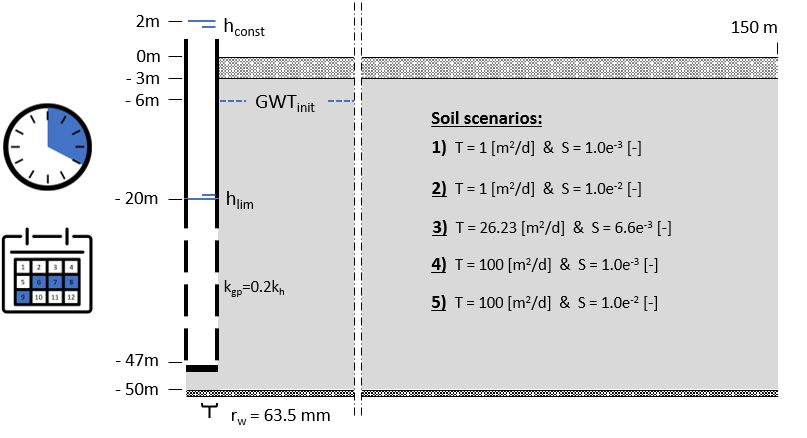
\includegraphics[width=0.7\linewidth]{Schematic_base_model}};  
\node[title, right=10pt] at (box.north west) {Schematic base model \& soil scenario definition};
\end{tikzpicture}
\captionsetup{justification=centering}
\caption{Schematic base model \& soil scenario definition}
\label{fig:Schematic_base_model}
\end{figure}

%
%\tikzstyle{mybox} = [draw=black, fill=white, very thick,
%    rectangle, rounded corners, inner sep=20pt, inner ysep=20pt]
%\tikzstyle{title} =[fill=black, text=white]
%
%\begin{figure}[h]
%\centering
%\begin{tikzpicture}
%\node [mybox] (box){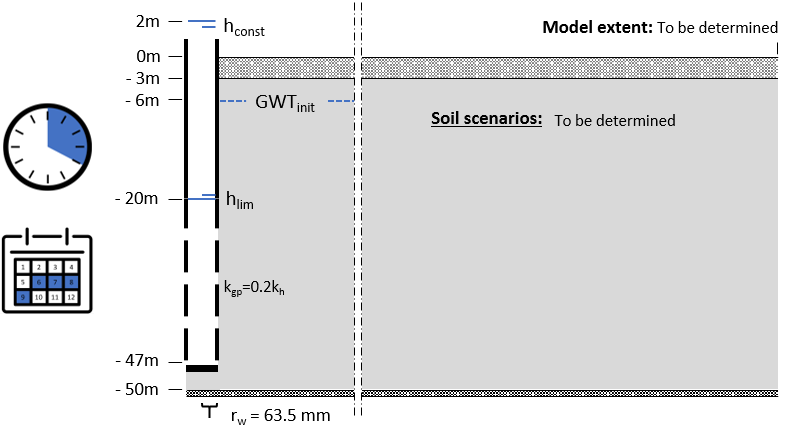
\includegraphics[width=0.7\linewidth]{Schematic_base_model_empty}};  
%\node[title, right=10pt] at (box.north west) {Schematic base model (reference)};
%\end{tikzpicture}
%\captionsetup{justification=centering}
%\caption{Schematic base model (reference)}
%\label{fig:Schematic_base_model_empty}
%\end{figure}

\textbf{Subsurface} \\
The interaction between the ASR system and the upper 50 m of subsurface is simulated. The model top is bounded by a 3m-thick poor permeable soil layer. The well penetration (partially) occurs in the underlying 47m-thick single aquifer. With an elevation of -6 m the initial groundwater table (GWT) is positioned just under the aquifer top. Unconfined conditions are applicable. The characteristic $T$ and $S$ values, defined in the soil scenarios of Section \ref{subsection:soil_sc_def}, apply to this aquifer. The aquifer is assumed to be homogeneous and horizontally isotropic, while the vertical anisotropy is 1/4 (-). The model extent is defined in correspondence with the obtained results from fieldwork data analysis. With a radial length of 150 m, the model scope is assumed to be sufficient. More information on the derivation of the extent can be found in Appendix \ref{section:Leakage_factor}. \\

%The results of the fieldwork data analysis ( for one or more layer(s), determined in Chapter \ref{chapter:Fieldwork_data_analysis}) are stated to be used as input for the definition of (multiple) soil scenarios. The exact applied soil scenarios are defined at the start of Chapter \ref{chapter:model_scenarios}. Subsequently, the model extent (radial distance from well) is based on these outcomes. More information on the definition of the radial extent can be found in Appendix \ref{section:Leakage_factor}.\\

\textbf{Well dimensions \& pump placement} \\
The base model design accommodates a single well with a radius of 0.0635 m (2.5 inch) and a total length of 47 m. It is assumed, in-well accumulation of sedimentation is absent. The displacement of water between well and aquifer is possible through a partially penetrating screen. Well screen perforation are present from 20 m to 47 m below the model top (screen length 27 m). More details on the well hydraulic conductivity can be found below. Dry season groundwater withdrawal is possible through the installation of a pump. The model contains a submergence pump positioned in the well at an elevation of -30 m. The maximum drop in GWT is limited to an elevation of -20 m (14 m drawdown relative to initial conditions). In this way the occurrence of well screen dry-out and pump malfunctioning is prevented. \\

\textbf{Well hydraulic conductivity} \\
Due to the tiny nature of screen perforations (and constructional soil around the borehole), a well skin resistance (hydraulic conductance) is taken into account. In this research the well hydraulic conductance is defined by the use of Equations \ref{eq:cond} - \ref{eq:K_skin}. 

\begin{equation}
 cond = \frac{2\pi r_w b}{c_{skin}}
\label{eq:cond}
\end{equation}

\begin{equation}
 c_{skin} = \frac{\Delta r_{skin}}{K_{skin}}
\label{eq:c_skin}
\end{equation}

where $cond$ (m$^2$/d) is the well hydraulic conductance, $r_w$ (m) is the radius of the well, $c_{skin}$ (d) is the well skin resistance , $\Delta r_{skin}$ (m) is the well skin (radial) length and $K_{skin}$ (m/d) is the well skin hydraulic conductance. \\

As stated by \citet{Houben2015}, the hydraulic conductivity of a sequence of materials (i.e. well screen, gravel-pack and aquifer) can be calculated by Equation \ref{eq:K_tot} (1D flow assumed). The model well cells are in this research defined in correspondence with the (radial) well dimensions (Appendices \ref{chapter:Extense_Modflow_model} \& \ref{MODFLOW_radial}). Therefore, the well skin conductance is assumed to be dependent on the materials of the well screen and the gravel-pack only. In this case, the well skin hydraulic conductivity corresponds with the simplified variant of Equation \ref{eq:K_tot}; Equation \ref{eq:K_skin}.  

\begin{equation}
 K_{tot} = \frac{\Delta r_{tot}}{\frac{\Delta r_{sc}}{K_{sc}} + \frac{\Delta r_{gp}}{K_{gp}} + \frac{\Delta r_{aq}}{K_{aq}}}
\label{eq:K_tot}
\end{equation}

\begin{equation}
 K_{skin} = \frac{\Delta r_{skin}}{\frac{\Delta r_{sc}}{K_{sc}} + \frac{\Delta r_{gp}}{K_{gp}}}
\label{eq:K_skin}
\end{equation}

where $K_{tot}$, $K_{skin}$, $K_{sc}$, $K_{gp}$ and $K_{aq}$ (m/d) are respectively the total, the well skin, the well screen, the gravel-pack and the aquifer hydraulic conductivities and ${\Delta r_{tot}}$, ${\Delta r_{skin}}$, ${\Delta r_{sc}}$, ${\Delta r_{gp}}$, ${\Delta r_{aq}}$ (m) are the corresponding (radial) length intervals of these materials. \\

The well skin length ($\Delta r_{skin}$) equals the summed up length of the well screen ${\Delta r_{sc}}$ and the gravel-pack ${\Delta r_{gp}}$. An ASR system well screen length of 0.005 m is measured in-field. The radius of the soil around the well, the gravel-pack, is undetermined. As stated by \citep{Bot2016}, for proper installation a minimum length of 0,125 m is required. This length is assumed and implemented in research. \\
The well skin hydraulic conductivity ($K_{skin}$) accounts for the combined conductivity of the well screen (perforations) and the gravel-pack around the well. The hydraulic conductivity of the well screen ($K_{sc}$) is based on research done by \citet{Houben2015}. Perforation sizes (screen slot width) of 2 mm are measured (study site investigation). These screen sizes correspond with a (clean) hydraulic conductivity ($K_{sc}$) of 1 m/s \citep{Houben2015}. As stated by \citet{LeonardF.KonikowGeorgeZ.HornbergerKeithJ.Halford2009}, the well skin hydraulic conductivity ($K_{skin}$) is typically expected to be lower than the aquifer hydraulic conductivity ($K_{h}$). To meet this requirement, the gravel-pack is interpreted as mildly clogged. The gravel-pack hydraulic conductivity ($K_{gp}$) is assumed to be 1/5 of the, soil scenario dependent, aquifer hydraulic conductivity ($K_{h}$). \\

%(Equation \ref{eq:cond}). The well skin resistance ($c_{skin}$) is inversely proportional to the well skin hydraulic conductivity ($K_{skin}$). The well skin hydraulic conductivity is typically lower than the original aquifer hydraulic conductivity ($K_{h}$)  \citep{LeonardF.KonikowGeorgeZ.HornbergerKeithJ.Halford2009,Houben2015}. A base model well skin hydraulic conductivity that equal 1/5 of the aquifer hydraulic conductivity is assumed. The definition of the well skin resistance is detailed described in


\textbf{Time frame} \\
As stated by the \citet{HAP2011}, the northern Ghana regions encounter a single wet season of approximate four months (dependent on the year and altitude) annually. Randomly applied interviews with local inhabitants (site visits) confirmed the temporal resolution of the wet season. Inundation levels of 0.5 m - 4 m are perceived with a timespan varying from weeks till the four months duration of the wet season (Appendix \ref{chapter:fieldworkresults}). \\
Seasonal system performance is simulated by a year-round (long term) temporal model resolution. In the synthetic (simplified) model it is assumed the region encounters flooding for as long as the wet season. A flood duration of four months is taken into account, starting on June 1$^{st}$ and ending on September 30$^{th}$. The flooding is simulated by gravity based infiltration on top of the ASR system. A constant (122 days) 2 m inundation level is assumed (Figure \ref{fig:Schematic_base_model}). In the subsequent eight months of dry season (October-May) no flooding or rainfall is taken into account. In accordance with the data obtained in the ASR system monitoring and interviews with farmers, groundwater withdrawal takes place by four hours of pumping daily. Intermediate day time offers time-space for recovery of the local GWT. For the purposes of this research it is assumed the hypothetical groundwater withdrawal last for as long as the dry season (243 days). \\

%These results are determined in subsequent parts of research (Chapter ). As a follow-up, the soil sceanrios applied in simulation are Chapter \ref{}  the or the  bandwidth of transmissivity and storativity values (derivatives from fieldwork data analysis (Chapter \ref{Fieldwork_data_analysis})), is used for the definition of five aquifer scenarios. An overview of the applied scenarios can be found in Figure \ref{fig:Schematic_base_model}).  These conditions are the base for the simulation of unsteady state flow in the radial and vertical direction.

\textbf{Model discussion} \\
The research base model results do not apply to a single research location (depicted in Figure \ref{fig:Overviewlocations}). The applied simplified model conditions serve research purposes. Assumptions made, are not by definition realistic. One can for example imagine the actual wet season inundation levels will fluctuate over time. And in practice, groundwater withdrawal needs day-specific tuning (not constant for 243 days) with respect to agricultural needs. Aspects advisable to take into account in further research.\\

%Obtained results should only be interpreted as indicative (improvement) options in northern Ghana ASR-system application. 

\textbf{Modelling environment - MODFLOW} \\
The computational modelling of the research synthetic ASR system is done with Modular Ground-Water Flow Model (MODFLOW), a finite difference model for groundwater flow developed by the U.S. Geological Survey (USGS). MODFLOW is the international standard in groundwater simulation \citep{Niswonger2011,HarbaughArlen2005}. More information on the applied inputs can be found in the Appendices \ref{chapter:Extense_Modflow_model} - \ref{MODFLOW_radial}.

%In the case of fieldwork data analysis  MODFLOW is not used for the derivation of geohydrological parameters. Optimal parameters derived with TTim models are implemented in corresponding MODFLOW models to validate obtained TTim results. More information on the modelling part can be found in Appendix.

\subsection{ASR system improvements}
\label{subsec:improvements}
A free interpretation of the term 'improvement' learns that multiple directions of ASR system modifications are applicable. As stated by \citet{Bakker2010} and \citet{Ward2007}, the success and sustainability of an ASR system is amongst others dependent on the length of injection, storage and recovery; the well dimension; and potential clogging of the well screen. In correspondence, the synthetic model of this research is exposed to three types of ASR system improvement:

\begin{itemize}
\item{a) Extension of daily pumping time:} \\
In a consecutive order the base model dry season pumping time (4 hours daily) is increased (by 1 hour steps) up to a maximum daily (dry season) pump operation of 8 hours.
\item{b) Enlargement of borehole cross-sectional dimension:} \\
The base model radius (0.0635m) is stepped up (doubled, tripled, etcetera) to in total five times its original radius: 0.3175 m. 
\item{c) Reduction of well skin resistance:} \\
This type of synthetic model improvement is designed by the application of enlarged gravel-pack hydraulic conductivities. In four equal steps (steps of (2/5)*$K_{h}$) the base model gravel-pack hydraulic conductivity ($K_{gp}$) is increased to a maximum of (9/5)*$K_{h}$. Note, well skin hydraulic conductivities larger than the aquifer hydraulic conductivities are considered in this way.
\end{itemize}

% More information on the calculation of the well skin conductance / resistance is stated in the Equations \ref{eq:cond} - \ref{eq:K_skin}.

\subsection{ASR system sensitivities}
\label{subsec:sensitivity}
The forces of northern Ghana's nature can highly fluctuate spatially and temporarily. Nonetheless, the base model houses multiple assumptions that are more or less fixed representations of nature (\ref{base_model_def}). A sensitivity analysis is part of the research to balance the impact of these assumptions. Three types of model modifications are part of the sensitivity analysis: 

\begin{itemize}
\item{a) Degradation of well depth (clogging):} \\
The study site observations imply that ASR systems in northern Ghana can be vulnerable for the power of nature. Due to the accumulation of sedimentation the well penetrations depths can decrease over time. The reduction is (simplified) simulated by a decrease in the well screen length. An hypothetical initial screen length of 30 m (longer than base model) is reduced in 5 m steps to a total screen length of 10 m.
\item{b) Shortening the wet season inundation timespan:} \\
Within northern Ghana the duration of the wet season is spatially dependent \citep{HAP2011}. Besides, season durations naturally differ between years. Through the application of three research steps, the synthetic base model wet season duration is reduced from four months (Jun-Sept) till one (Aug).  
\item{c) Reduction of wet season inundation level:} \\
The impact of lower inundation levels is analysed in combination with increased initial groundwater tables. Relative to the base model ($\Delta h$ is 8m) the $\Delta h$ is reduced (in steps of 2 m) to a minimum of $\Delta h$ is 2 m.   
\end{itemize}

%\begin{itemize}
%\item{a) Degradation of well depth (clogging):} \\
%The fieldwork observations imply that ASR systems in northern Ghana can be vulnerable for the power of nature. Due to the accumulation of sedimentation the well penetrations depths can decrease over time. The reduction is simulated by a decrease in the well screen length. An hypothetical initial screen length of 30 m is reduced (steps of 5 m) to 10 m.
%\item{b) Shortening the wet season inundation timespan:} \\
%Within northern Ghana the duration of the wet season is spatially dependent \citep{HAP2011}. Besides, season durations naturally differ between years. Through the application of three steps the synthetic base model wet season duration is reduced from four months till one.
%\item{c) Reduction of wet season inundation level:} \\
%Different flood inundation levels are encountered by local inhabitants. As mentioned by the \citet{HAP2011}, wet season intensities vary within northern Ghana. Besides, initial groundwater tables are not fixed. Based on the fieldwork inspection it is confirmed that the GWT in northern Ghana varies. The impact of lower inundation levels is analysed in combination with increased initial groundwater tables. Relative to the base model ($\Delta h$ is 8m) the $\Delta h$ is reduced (in steps of 2 m) to a minimum of $\Delta h$ is 2 m.   
%\end{itemize}

%At all study site locations (\ref{section:research_locations} measured borehole depths are less than original. The accumulation of sedimentation reduces the active borehole depth over time.  the borehole depth decreases due to the (e.g. ASR system location Nungo)   bldednhecnecdnennenqcnnencncbbcecbcbcbcjbcbcjcj

\subsection{Test criteria - sustainability}
As mentioned in Section \ref{base_model_def}, the synthetic ASR system performance is simulated in the time-frame of a year. A distinction can be made between the wet and dry season. The wet season ASR system functionality is characterized by the groundwater recharge. Analysis is pointed at the inflow volumes and the impact of these volumes on the GWT. In the subsequent eight months of dry season, the system works in reverse. In this time of year, maximum pump operation and the accompanied impact on GWT is of key interest. \\
As a supplement, the mutual relation between recharge and discharge is considered. This is done by the introduction of the 'Recovery ratio' $R_{\%}$ (Equation \ref{eq:RR}). The Recovery ratio is similar to Recovery Efficiency (RE) applied by \citet{Ward2007}. \citet{Ward2007} mentions the RE ($R_{\%}$) is a measure to indicate the degree of recovery, i.e. RE = 1 (-) (100\%) implies complete recovery. 

\begin{equation}
 R_{\%} = \frac{V_{out,tot}}{V_{in,tot}}
\label{eq:RR}
\end{equation}

Where  R$_{\%}$ is the year-round Recovery Ratio (-), $V_{in,tot}$ (m$^3$) is the wet season total volume recharged and $V_{out,tot}$ (m$^3$) is the dry season total volume discharged. \\

The ASR system sustainability is discussed through the Recovery ratio. A $R_{\%}$ smaller than 1 (-) indicates a year round net inflow. In this case, the interaction between system and nature is positive. For the purposes of this research 'sustainability' is defined as a situation where the $R_{\%}$ is smaller than or equal to 1 (-). The potential increase in groundwater withdrawal, due to synthetic improvements, is bounded by sustainability. In other words, a 100\% recovery is set as an upper system limit. \\


%northern Ghana parameter test problem contains a fictive, simplistic ASR-system in northern Ghana. Year-round well performance due to water infiltration and extraction is modelled. Applied conditions are based on local fieldwork measurements. Model results do not apply to a single research location (depicted in Figure \ref{fig:Overviewlocations}). Obtained results should only be interpreted as indicative (upscaling) options in northern Ghana ASR-system application.
%
%\subsection{Soil scenarios} 
%Interaction between the ASR-system and the upper 50 m of subsurface is simulated. Model top is bounded by a 3m-thick poor permeable soil layer. Well penetration occurs in the underlying 47m-thick aquifer. With an elevation of -6 m the initial groundwater table (GWT) is positioned just under the aquifer top (unconfined). The aquifer is homogeneous and horizontally isotropic, while a vertical anisotropy of 1/4 (-) is assumed. The bandwidth of transmissivity and storativity values (derivatives from fieldwork data analysis (Chapter \ref{Fieldwork_data_analysis})), is used for the definition of five aquifer scenarios. An overview of the applied scenarios can be found in Figure \ref{fig:Schematic_base_model}).  These conditions are the base for the simulation of unsteady state flow in the radial and vertical direction.
%
%
%\subsection{Performance}
%Base model design (not subjected to upscaling) accommodates a single well with a radius of 0.0635 m (2.5 inch). Water displacement between well and aquifer is possible through a partially penetrating screen. Well skin perforation are present from 20 to 47m below model top. It is assumed the, in total 27 m, screen is clean. Due to the tiny nature of wall perforations (and constructional soil improvement around the borehole) a well skin resistance is taken into account. More information on skin resistance is included in Section \ref{section:MODFLOW_const}. Dry season groundwater withdrawal is possible through the installation of a pump. The model contains a pump at an elevation of -30 m. A drop in GWT is preferable limited to an elevation of -20 m (14 m drawdown relative to initial conditions). In this way the occurrence of well screen dry-out and pump malfunctioning is prevented.
%
%\subsection{Time frame} 
%ASR-systems can theoretically add value to groundwater availability constantly. Seasonal system behaviour is simulated by a year-round (long term) temporal model resolution. For a duration of four months, starting on June 1$^{st}$, gravity based infiltration simulates wet season flooding. A constant (122 days) 2 m inundation level (on top of well) is assumed (Figure \ref{fig:Schematic_base_model}). In the subsequent eight months of dry season no flooding or rainfall is accounted. Dry season water withdrawal takes place by four hours of pumping daily (243 days). Intermediate day time offers time-space for GWT recovery. \\

\section{ASR system base model performance}
\label{section:Base_model_perf}
In the methodology all the model components are set to simulate and study the potential improvements of an ASR system. As a reference, this section contains a description of the year-round base model performance in combination with the different soil scenarios.

\subsection{Wet season}
The four months of wet season are simulated by the instantaneous occurrence of a (2 m constant) flooding on top of the ASR system. The difference between the level of inundation and the groundwater table (GWT initially -6 m) results in a gravity based groundwater recharge. At simulation start the head difference (hydraulic gradient) is highest. In correspondence, the initially observed inflow is above average. Due to the mutual interaction, the recharge causes the GWT to increase. The hydraulic gradient mutes over time. In the first days (approximately five days) the hydraulic gradient declines fast. Thereafter, the decline remains present but progresses excessively slow. Although the inflow does not reach a steady state, the rate of water accumulation in the aquifer is close to constant for the time-scope of this research (four months). This system performance is visualized for soil scenario 3 in the Figure \ref{fig:Sens_delt_Sc3_recharge_time} and \ref{fig:Sens_delh_Sc3_recharge_time}, but takes place in all soil scenarios. As an visual example of the wet season flood impact on groundwater, the soil scenario 3 radial cross-sectional head contours at the begin (day 5) and absolute end of wet season (day 122) are presented in Figure \ref{fig:Example_Sc3_base_cont_wet}.

\begin{figure}[h!]
	\centering
	\begin{subfigure}[b]{0.5\linewidth}
		\centering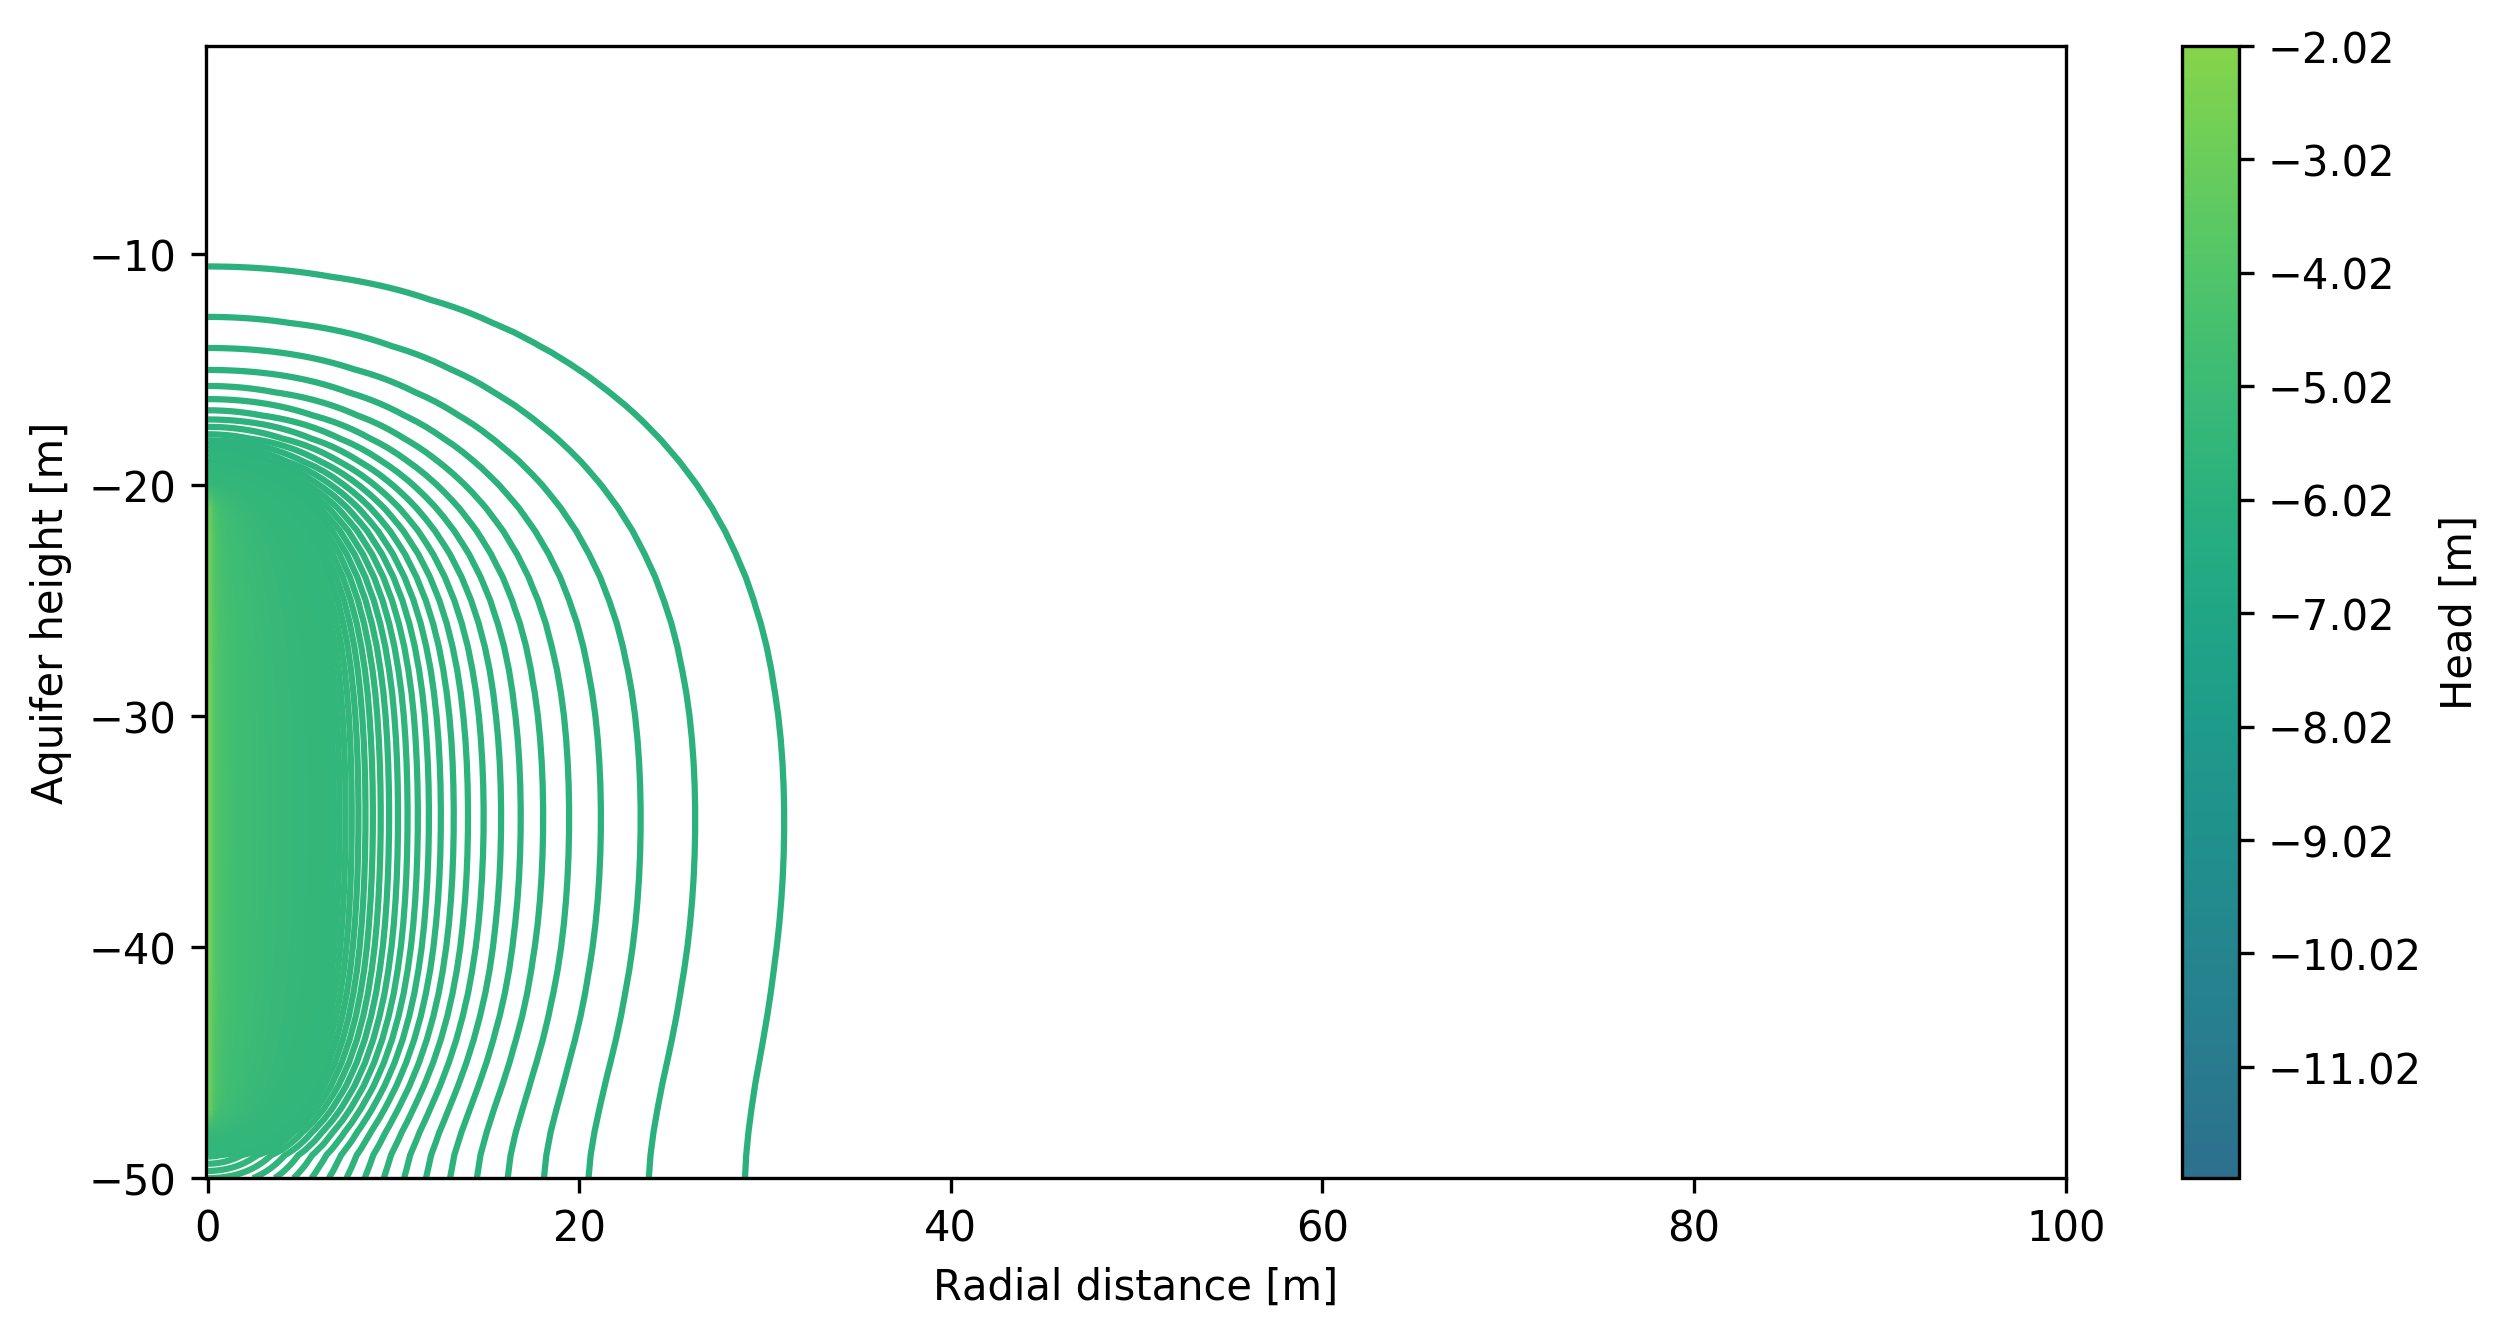
\includegraphics[width=\linewidth]{Sc3a1_cont_d5}
		\captionsetup{justification=centering}		
		\caption{\label{fig:Sc3a1_cont_d5}}
		\end{subfigure}\hfill
	\begin{subfigure}[b]{0.5\linewidth}
        \centering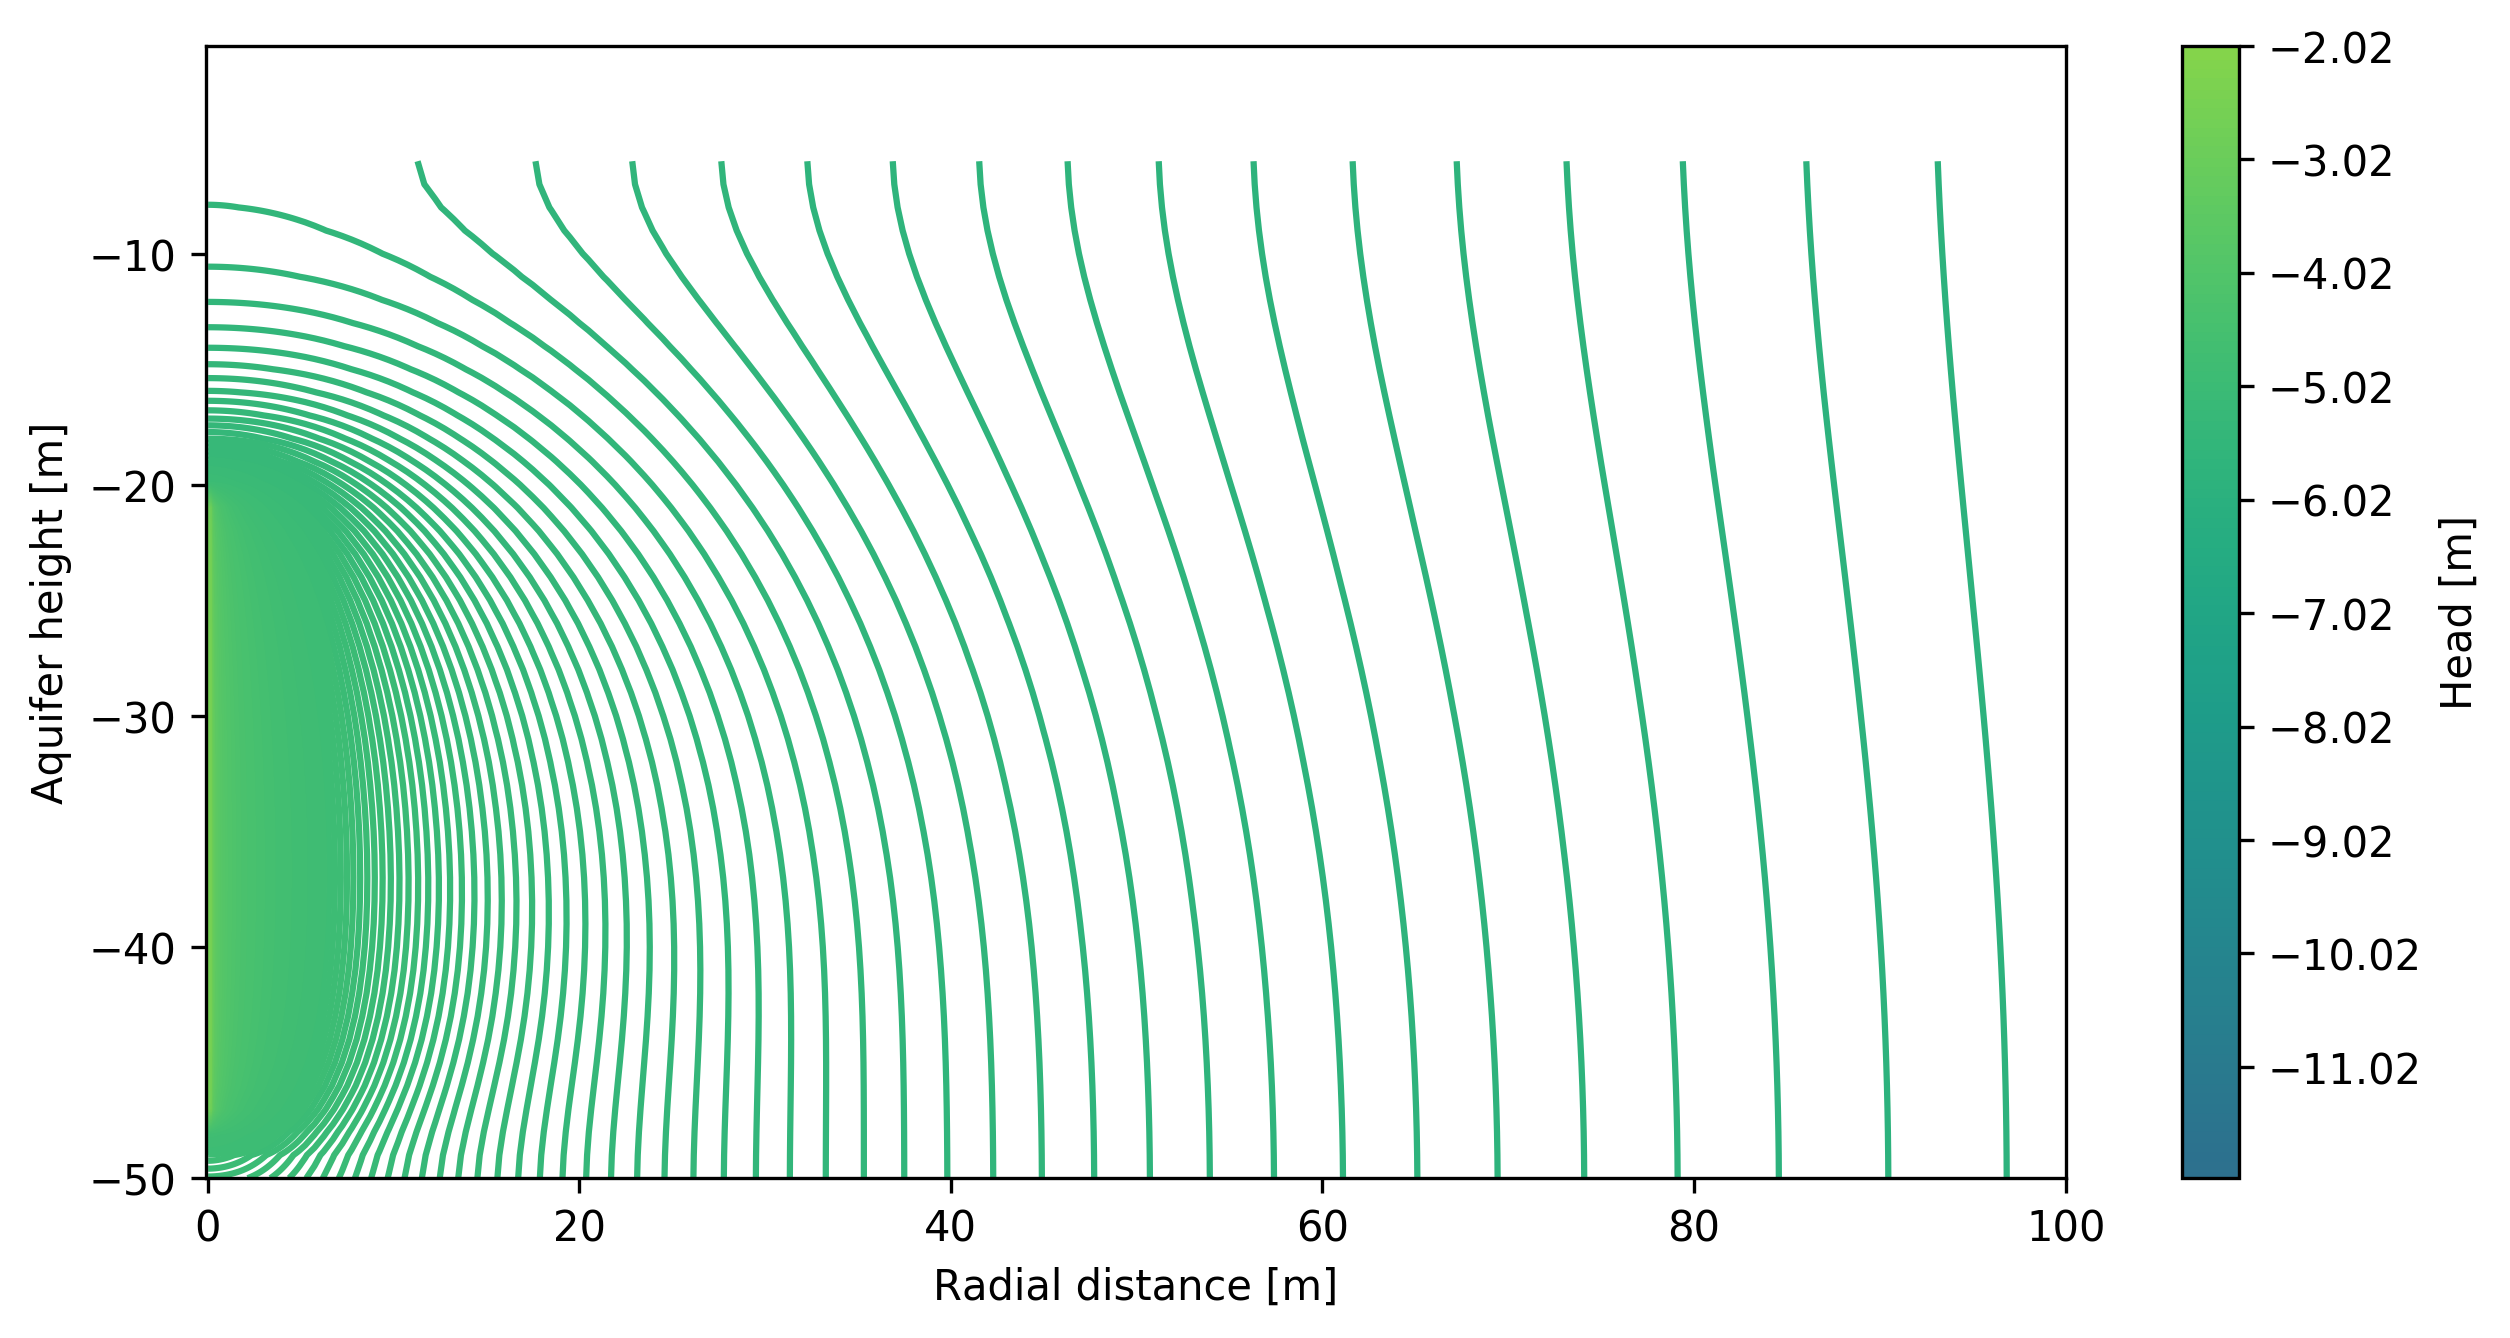
\includegraphics[width=\linewidth]{Sc3a1_cont_d122}
		\captionsetup{justification=centering}		
		\caption{\label{fig:Sc3a1_cont_d122}}
		\end{subfigure}
		\captionsetup{justification=centering}	
	\caption{Base model soil scenario 3- Cross-sectional contour head after (\subref{fig:Sc3a1_cont_d5}) five days and (\subref{fig:Sc3a1_cont_d122}) 122 days of infiltration} 
	\label{fig:Example_Sc3_base_cont_wet}
\end{figure} 

%Impacts on the groundwater table are also dominant at simulation front. At close well range relative large increases in groundwater heads are encountered in the first days.
A significant (more or less instant) head increase is encountered at close well (screen) range. The groundwater head does not reach the predefined flood level, not even at end of the wet season. A performance that can be attributed to the implemented well skin resistances. In terms of radial distance the system impact (on GWT) remains limited. After 122 days of infiltration the head increase is not quite substantial at a distance of approximately 60-80 m (in all scenarios). More visualizations on the base model performance can be found in Appendix \ref{section:base_performance}. \\

The scenario dependent results on total wet season inflow volumes are included in Table \ref{tab:Base_recharge}. Differences between the soil scenario 1 and 2 as well as the scenarios 4 and 5 are small. These soil scenarios only differ in the applied storativity (S) values. The variance in storativity (defined in bandwidth) appears to have only limited influence on the inflow of water, most definitely during the application of higher transmisivities. Nonetheless, the obtained absolute recharge volumes show significant differences between the entire spectrum of soil scenarios. These differences can be attributed to the applied soil scenario transmissivity values. 

\begin{table}[h!]
\small
\centering
\caption{Base model scenarios - Wet season recharge (m3)}
\label{tab:Base_recharge}
\begin{tabular}{l|r|r|r|r|r}
\hline 
\textbf{}               & \textbf{Sc 1} & \textbf{Sc 2} & \textbf{Sc 3} & \textbf{Sc 4}  & \textbf{Sc 5} \\ \hline \hline
Volume in (m$^3$)       & 207.57        & 208.68        & 5357.45       & 20330.33       & 20333.15          \\ \hline    
\end{tabular}
\end{table}

\subsection{Dry season}
The simulated well discharge (four hours dry season daily) originates by a predefined sustainable maximum withdrawal. In all soil scenarios, the obtained (base model) discharges do not exceed the limits of sustainability (visualized for soil scenario 3 in Figure \ref{fig:Example_Sc3_base_discharge}). Instead, the system performance is limited by the maximum allowed drawdown. The head bound (-20 m in well) is reached almost instantaneously after the start of pumping operation. In the subsequent hours of pumping (within day) the head bound keeps active. The simulation compensates by a decrease in discharge over time. In practice pumping takes place at a more or less constant rate. It suggests, modelled outcomes overestimate the discharge volumes slightly. Mutual comparison between the days shows a difference in total discharge between the first and all other days of pumping. The first day of pumping generates somewhat higher volumes. In the subsequent days discharge volumes are by approximation equal. \\

\begin{figure}[H]
	\centering
	\begin{subfigure}[b]{0.5\linewidth}
		\centering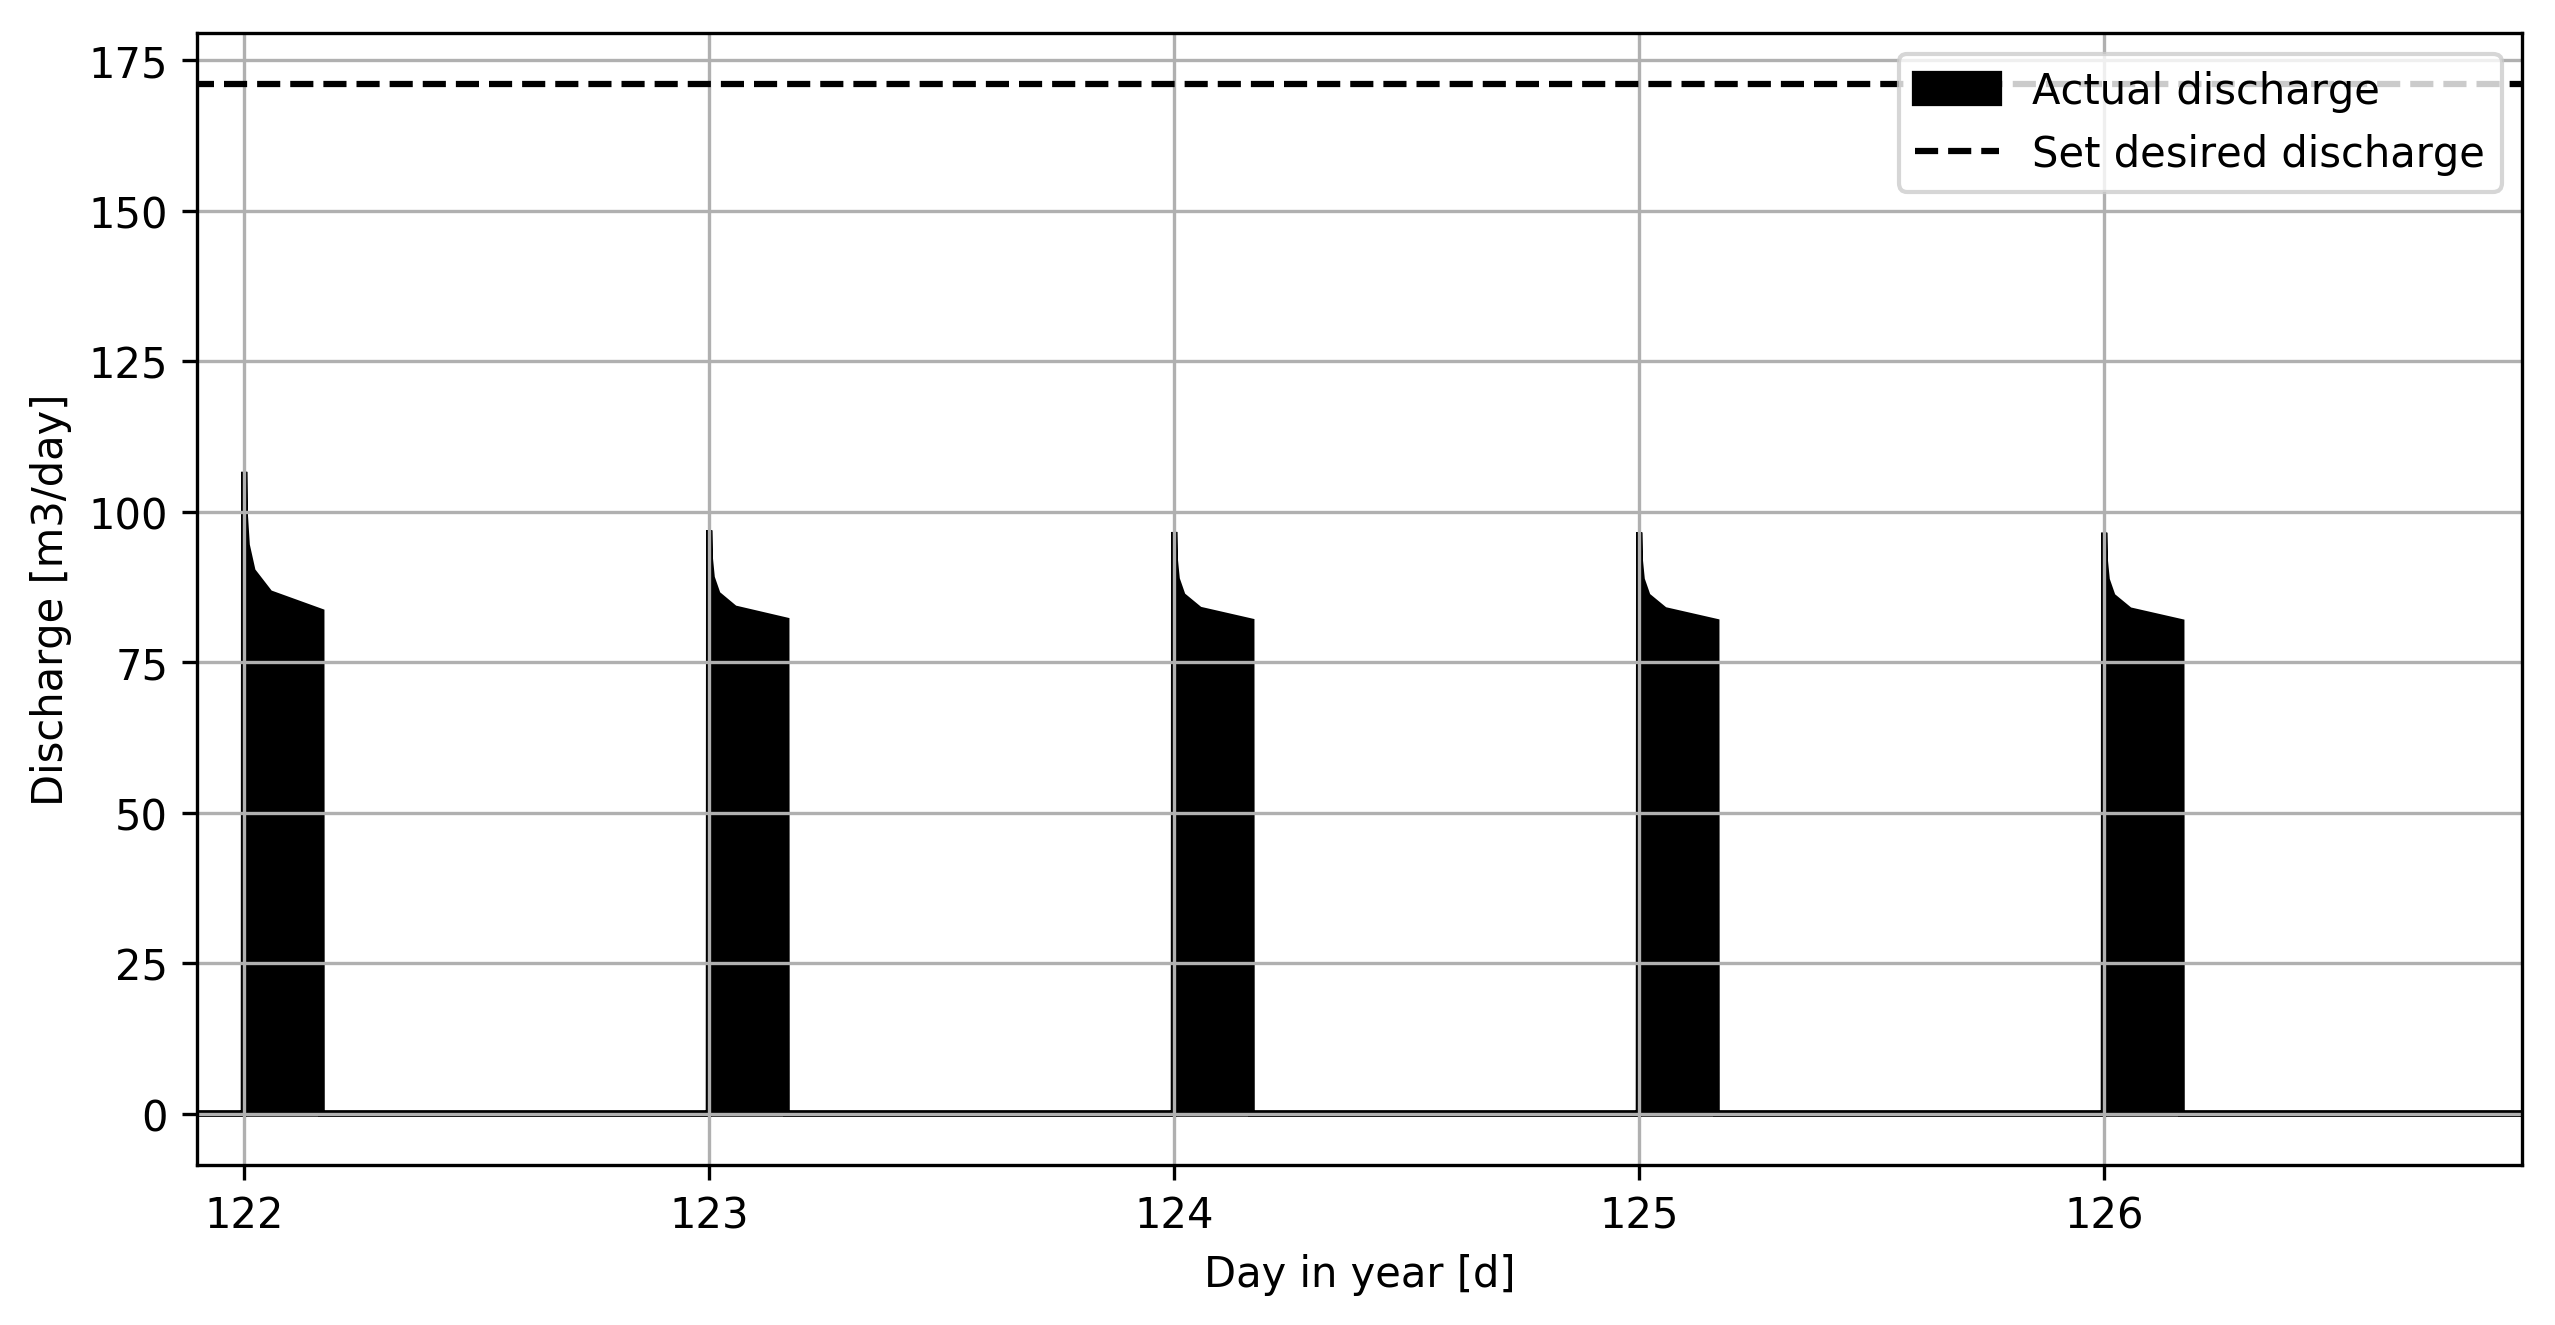
\includegraphics[width=\linewidth]{Sc3a1_Q122_126}
		\captionsetup{justification=centering}		
		\caption{\label{fig:Sc3a1_Q122_126}}
		\end{subfigure}\hfill
	\begin{subfigure}[b]{0.5\linewidth}
        \centering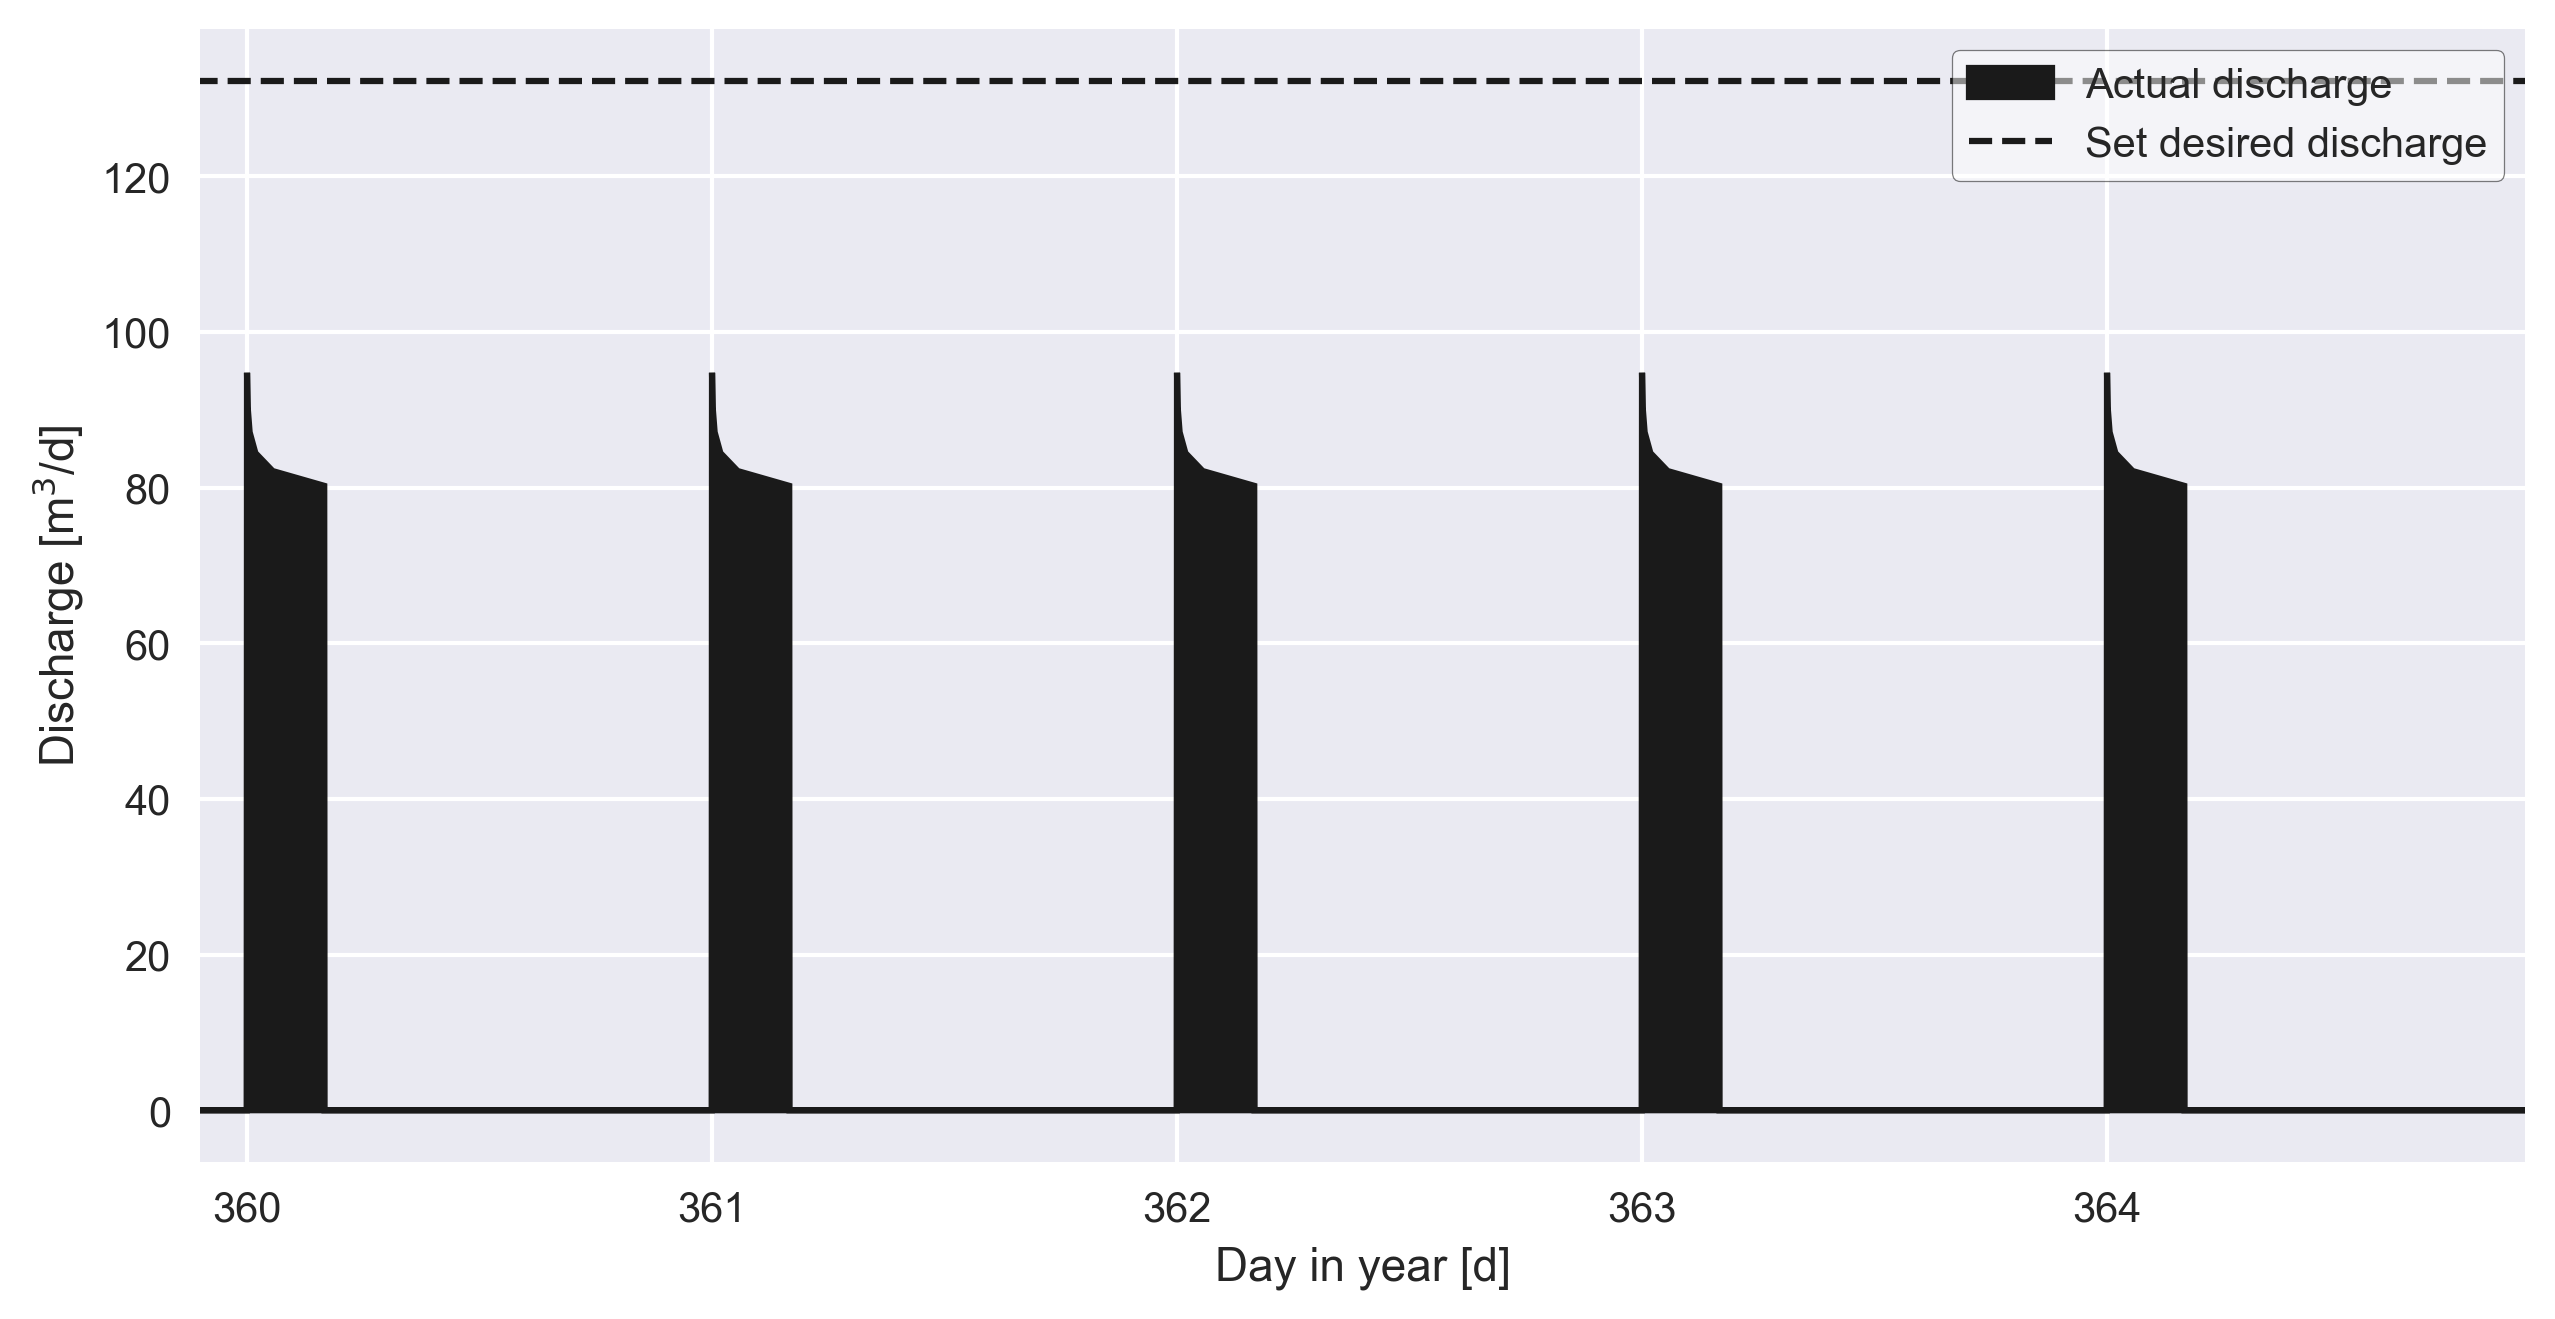
\includegraphics[width=\linewidth]{Sc3a1_Q360_364}
		\captionsetup{justification=centering}		
		\caption{\label{fig:Sc3a1_Q360_364}}
		\end{subfigure}
		\captionsetup{justification=centering}	
	\caption{Base model soil scenario 3 - Discharge performance for   (\subref{fig:Sc3a1_Q122_126}) the first five days and (\subref{fig:Sc3a1_Q360_364}) the last five days of dry season} 
	\label{fig:Example_Sc3_base_discharge}
\end{figure} 

The impact of well discharge on groundwater (example soil scenario 3) is presented in the cross sectional contour plot of Figure \ref{fig:Example_Sc3_base_cont_dry}. After the first day of pumping the transition from wet (recharge) to dry season (discharge) is still observable. Towards the end of the year this impact is no longer present. Over the entire dry season, the head bound (-20 m) is not reflected in the contour range. This can be justified by the influence of the well skin resistance. The maximum allowed drawdown is reached in the well. As a result, the consequences on nature (groundwater) are less distinctive. More visualizations on the base model performance can be found in Appendix \ref{section:base_performance}. \\

% dit onderstaande plaatje (van bovenstaande 2 in 1 krijg ik via python niet opgeslagen 

%\begin{figure}[h!]
% \centering
% \includegraphics[width=1.0\linewidth]{Sc3a1_Q}
% \captionsetup{justification=centering} 
% \caption{Example on scenario 3 - base model  - discharge performance - for the first and last five days of pumping}
% \label{fig:Example_Sc3_base_dis}
%\end{figure}

\begin{figure}[h!]
	\centering
	\begin{subfigure}[b]{0.5\linewidth}
		\centering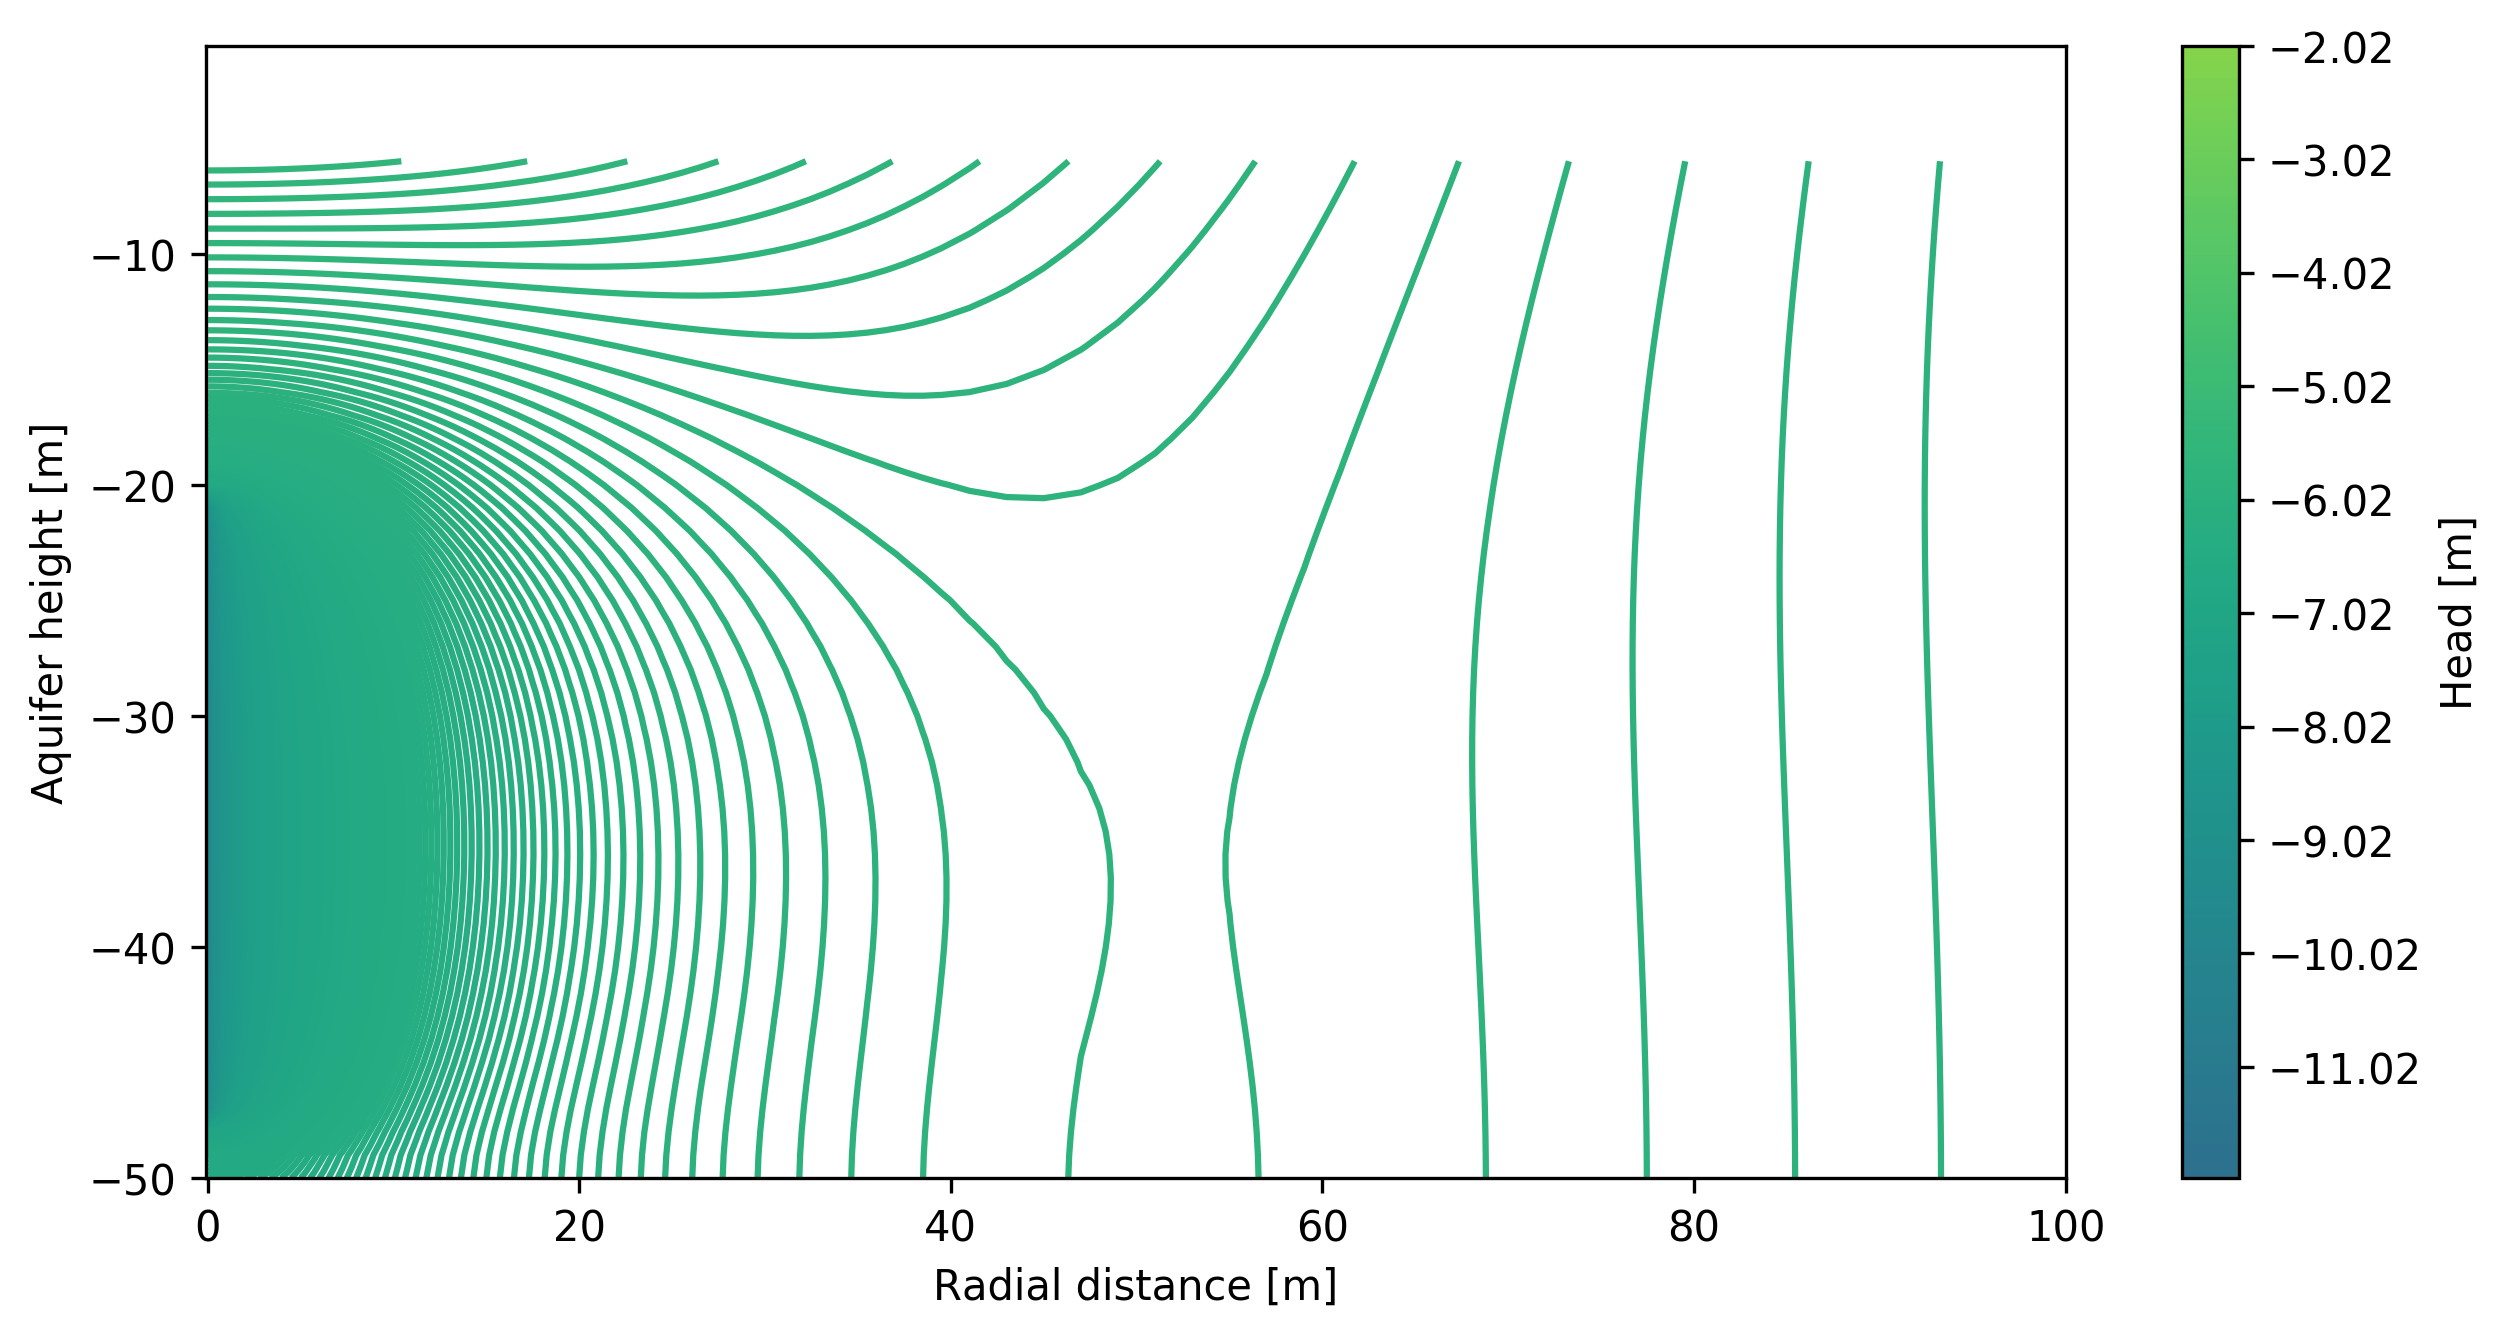
\includegraphics[width=\linewidth]{Sc3a1_cont_d123pump}
		\captionsetup{justification=centering}		
		\caption{\label{fig:Sc3a1_cont_d123pump}}
		\end{subfigure}\hfill
	\begin{subfigure}[b]{0.5\linewidth}
        \centering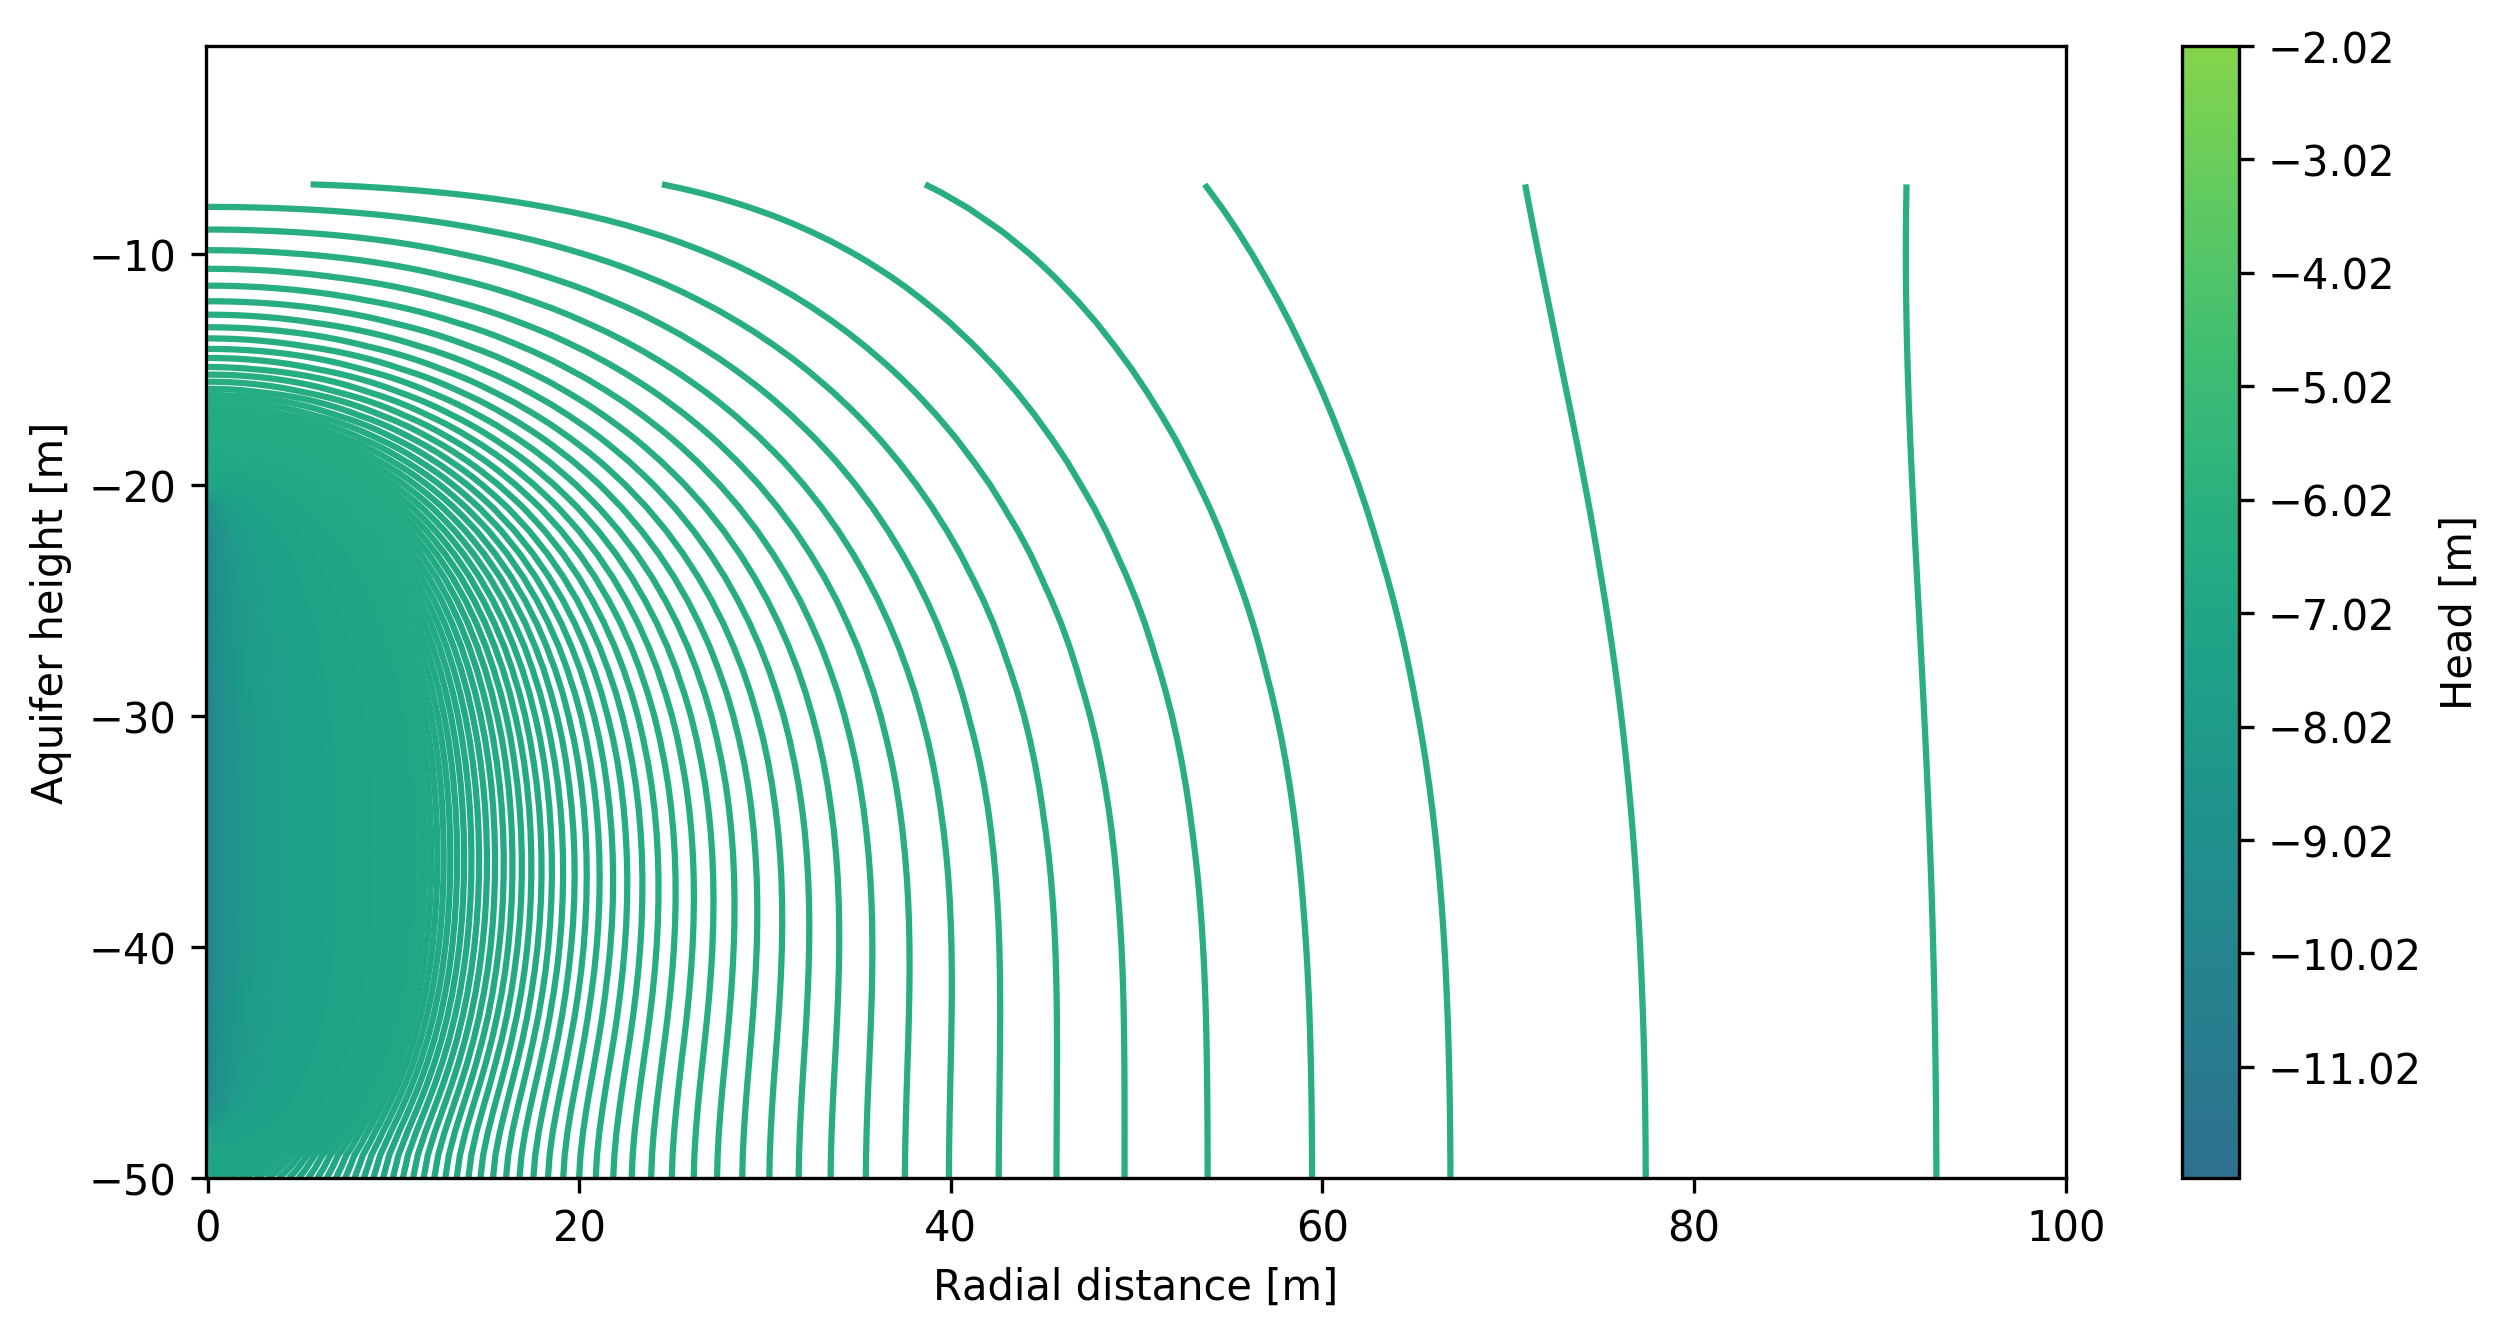
\includegraphics[width=\linewidth]{Sc3a1_cont_d364pump}
		\captionsetup{justification=centering}		
		\caption{\label{fig:Sc3a1_cont_d364pump}}
		\end{subfigure}
		\captionsetup{justification=centering}	
	\caption{Base model soil scenario 3 - Cross-sectional contour head after four hours of pumping on (\subref{fig:Sc3a1_cont_d123pump}) the first day (day 123) and (\subref{fig:Sc3a1_cont_d364pump}) the last day (day 365) of dry season} 
	\label{fig:Example_Sc3_base_cont_dry}
\end{figure} 

Unlike the outcomes in recharge, all different soil scenarios show (minor) distinctive results in total volumes discharged. The variation in storativity is possible more pronounced for discharge (after a certain time of recharge) than for recharge. However, the total volumes withdrawn are still in the same order of size for the scenarios 1 and 2, and the scenarios 4 and 5. The obtained discharges are in absolute terms more emphatically determined by the (range of) transmissivity values. 

\begin{table}[h!]
\small
\centering
\caption{Base model scenarios - Dry season discharge (m3)}
\label{tab:Base_discharge}
\begin{tabular}{l|r|r|r|r|r}
\hline 
\textbf{}               & \textbf{Sc 1} & \textbf{Sc 2} & \textbf{Sc 3} & \textbf{Sc 4}  & \textbf{Sc 5} \\ \hline \hline
Volume out (m$^3$)       & 129.84        & 137.76        & 3299.99       & 12080.08 	      & 12353.58          \\ \hline    
\end{tabular}
\end{table}

\subsection{Recovery ratio $R_\%$}
The Recovery ratios $R_\%$ are for all base models scenarios in the same order of size (Table \ref{tab:Base_RR}. Nonetheless, the positive outlier of soil scenario 2 is worth-mentioning. Mutual differences in performance can potentially be attributed to the varying storativity values (in combination with different transmissivity values). The ratios are also affected by the (soil scenario dependent) well skin resistances. As a consequence, no conclusions can be drawn on the scenario distinctive Recovery ratios. \\ 

\begin{table}[h!]
\small
\centering
\caption{Base model scenarios - Recovery ratio $R_\%$}
\label{tab:Base_RR}
\begin{tabular}{l|r|r|r|r|r}
\hline 
\textbf{}               & \textbf{Sc 1} & \textbf{Sc 2} & \textbf{Sc 3} & \textbf{Sc 4}  & \textbf{Sc 5} \\ \hline \hline
$R_\%$ (-)              &  0.626        & 0.660         & 0.616         & 0.594 	     & 0.608 	          \\ \hline    
\end{tabular}
\end{table}

In all base model soil scenarios the recovery ratio stays below 100\%. In eight months of daily (4 hours) pump operation it is not possible to fully recover the volumes infiltrated due to four months of constant inundation (2 meter) on top of the well. A reason for this is that the inflow bubble may level out over the aquifer due to the hydraulic gradient \citep{Bakker2010}. The discharge water is not by definition the 'original' recharge water. Under the defined conditions of system composition and use, the found Recovery ratios suggest a sustainable system use and impact on nature. \\

%\clearpage
\section{ASR system improvements}
\label{section:ASR_upscaling}
This section presents the impact of potential improvements of an ASR-system. One-by-one, different types of improvement are taken into account. The model performances are described by the test criteria: total recharge, discharge and Recovery ratio ($R_{\%}$). The results can be weighted to the base model. 

\tikzstyle{mybox} = [draw=black, fill=white, very thick,
    rectangle, rounded corners, inner sep=15pt, inner ysep=15pt]
\tikzstyle{title} =[fill=black, text=white]

\subsection{Extension of daily pumping time}
\label{Subsec:Up_time}
The extent of the daily (dry season) pumping operation is an easily applicable variant to improve the ASR system yield. Except from additional fuel and possibly temporal storage requirements (poly tanks), no further modifications are required. Base model pump operation is set to be four hours daily (243 days, dry season). This study is pointed at a maximum time-scope of pumping for 8 hours daily. As visualized in Figure \ref{fig:Schematic_up_time}, the system improvement is implemented in four simulation steps. 

\begin{figure}[h!]
\centering
\begin{tikzpicture}
\node [mybox] (box){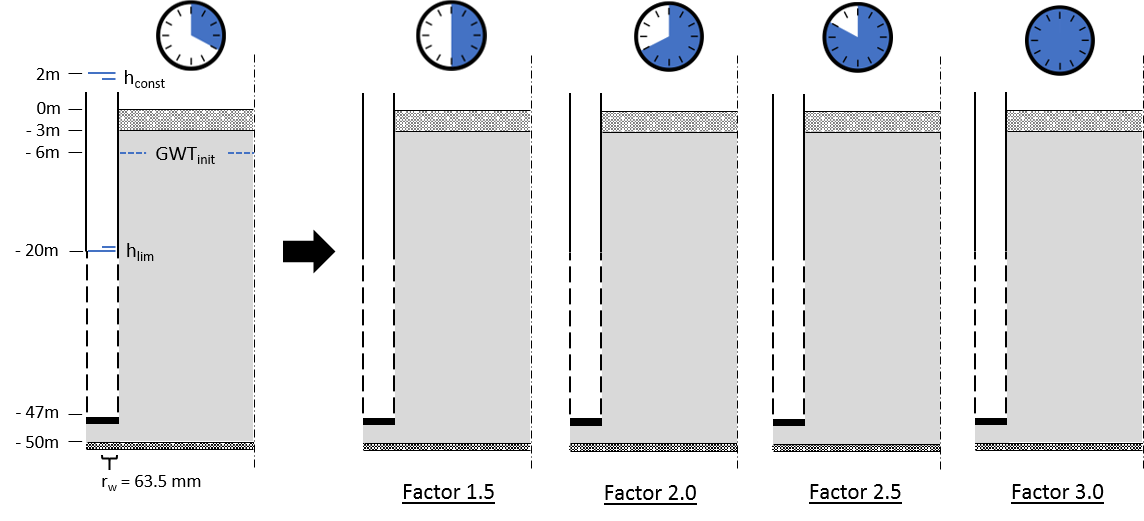
\includegraphics[width=0.9\linewidth]{Schematic_up_time}};  
\node[title, right=10pt] at (box.north west) {Schematic extension daily pumping time};
\end{tikzpicture}
\captionsetup{justification=centering}
\caption{Schematic extension daily pumping time}
\label{fig:Schematic_up_time}
\end{figure}

Deviations in wet season recharge are not applicable to this type of system improvement. Pump operation is only in effect during dry season. As visible in Figure \ref{fig:Results_up_time}, discharged volumes are most definitely affected by the duration of pumping. An approximately linear ascending relation is observed in all soil scenarios. The relation can be justified by the daily discharge performance, as depicted for the base model in Figure \ref{fig:Example_Sc3_base_discharge}. After four hours of pumping a more or less equilibrium (maximum) discharge rate is present. Extension by adding active hours of pumping daily will not make any significant change in discharge rates. Moreover, the discharge pattern is repeated daily. Except from the first day, mutual differences between the dry season days of pump operation are small. \\

\begin{figure}[h!]
 \centering
 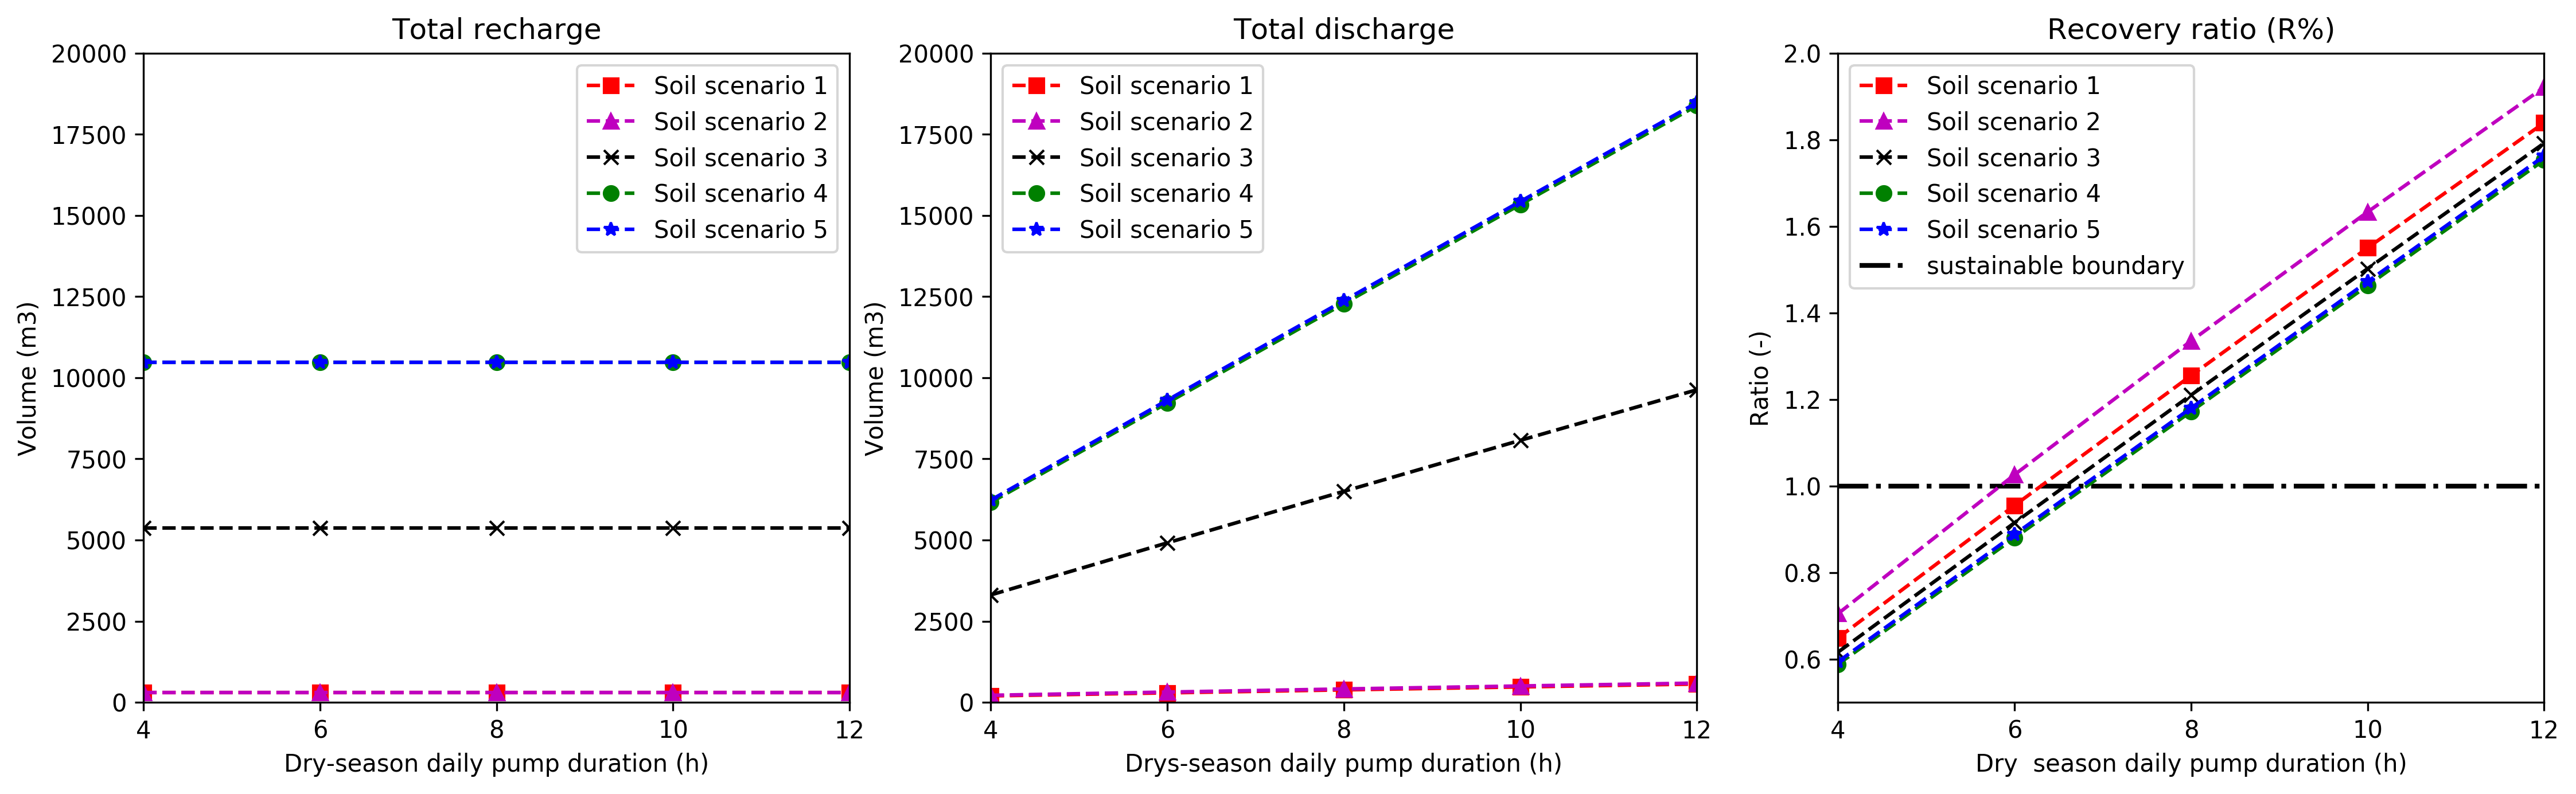
\includegraphics[width=1.0\linewidth]{Results_up_time}
 \captionsetup{justification=centering} 
 \caption{Results of yearly total volumes (in, out, ratio) by extension daily pumping time}
 \label{fig:Results_up_time}
\end{figure}

By the extension of the daily pumping time, the total discharge volumes (eight months) can equal (or exceed) the total inflow volumes (four months). A 100\% Recovery is in all soil scenarios obtained in the situation of 6 till 7 hours of dry season daily pumping operation. When base model conditions (2 m constant inundation for four months) apply, it is advisable pumping operations should not exceed the 6 till 7 hours duration (on daily basis). In this way, a sustainable system use can potentially be retained. \\

%on a dabecause of sustainabili By further extension of pump duration the potential negative effects on nature (unsustainable system use) should be considered.

\subsection{Enlargement of borehole cross-sectional dimension}
\label{Subsec:Up_diam}
The enlargement of the borehole cross-sectional dimension is a rigorous approach in the improvement of an ASR system. An adjustment that can not be applied on existing systems. If the appropriate equipment is present (e.g. drilling machinery), the enlargement can be applied by new constructions. To take implementation in consideration, it is of extra interest to gain knowledge on potential effects. The enlargement is tested by a stepwise (4 steps) multiplication of the original borehole radius (Figure \ref{fig:Schematic_up_diam}). 

\begin{figure}[h!]
\centering
\begin{tikzpicture}
\node [mybox] (box){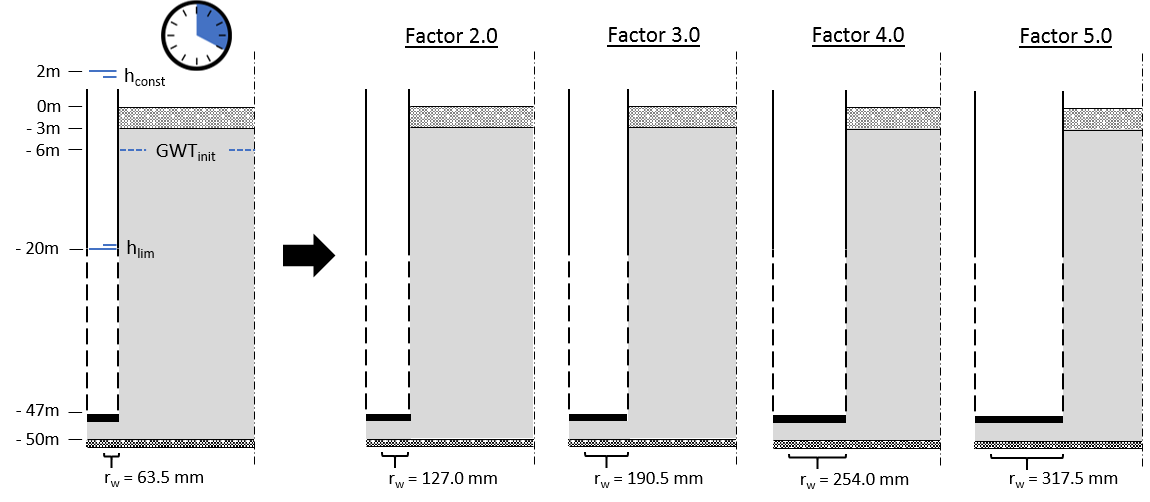
\includegraphics[width=0.9\linewidth]{Schematic_up_diam}};  
\node[title, right=10pt] at (box.north west) {Schematic enlargement borehole cross-sectional dimension};
\end{tikzpicture}
\captionsetup{justification=centering}
\caption{Schematic enlargement borehole cross-sectional dimension}
\label{fig:Schematic_up_diam}
\end{figure}

The magnification of the borehole diameter is beneficial for both groundwater recharge and discharge. In Figure \ref{fig:Results_up_diam}, it can be seen that a non-linear ascending relation is present between the ASR system diameter and the total inflow, outflow and Recovery ratio. Well-size improvement is beneficial, but an increasingly less positive effect is obtained. The cross-sectional enlargement is not endless, both in terms of volumes and practical application. In the scope of this research (five times the base model size) a volume increase well over two times its original is acquired. 

%With minor enlargement, large 'profit' can be achieved. A cross-sectional diameter of five times its original size, results in over two times the basemodel in- and outflow.

\begin{figure}[h!]
 \centering
 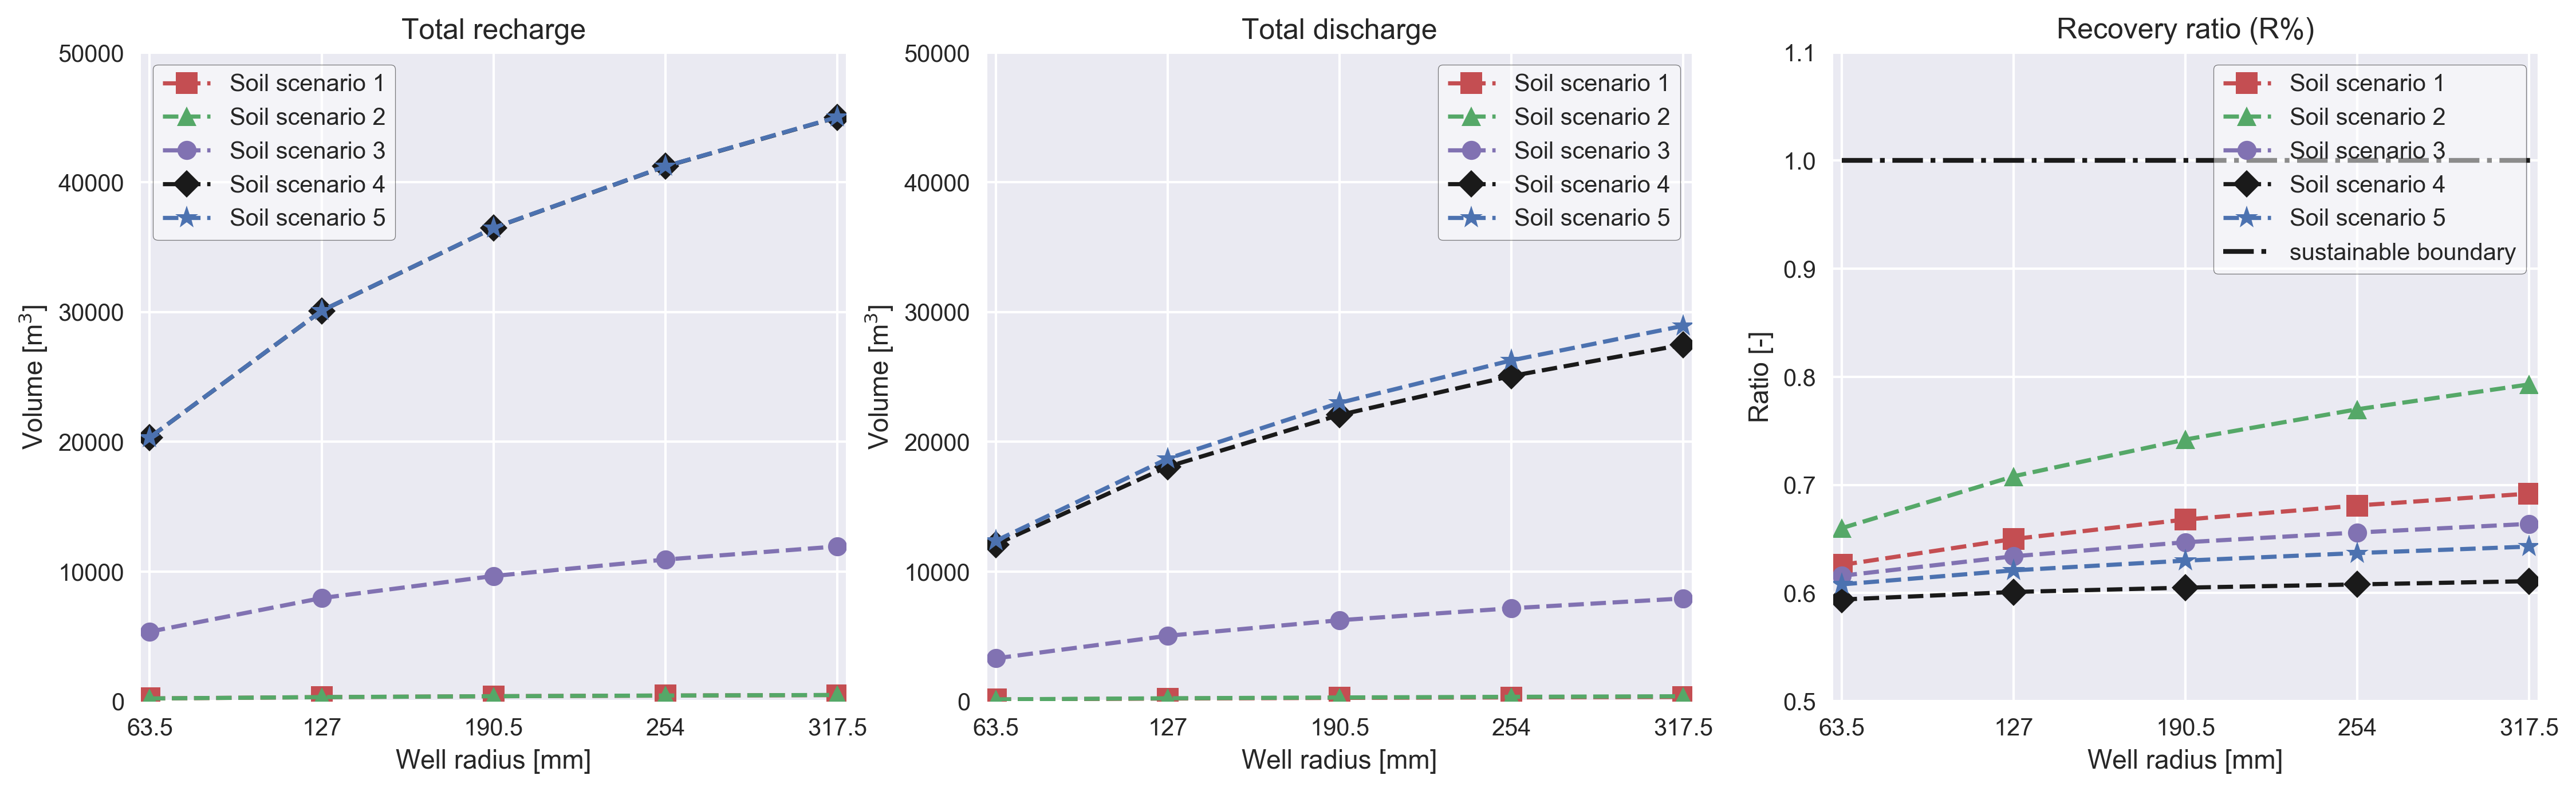
\includegraphics[width=1.0\linewidth]{Results_up_diam}
 \captionsetup{justification=centering} 
 \caption{Results of yearly total volumes (in, out, ratio) by enlargement well cross-sectional dimension}
 \label{fig:Results_up_diam}
\end{figure}

%Unforeseen performances are obtained in the recovery ratios of scaled-up simulation in scenarios 1 and 2. After solid ratio increase, further system upscaling suddenly causes a decline in recovery performance. Closer inspection exposed the cause. Recharge volumes continue to follow an upward trend, while total discharge volumes stay at the same level. The predefined desired discharge ($Q_thiem$) are reached in these scaled-up scenarios. Impact becomes transparent by the comparison of discharge performances of the (soil) scenario 1 base model versus the model simulation with an (5 times) increased well radius (Figure \ref{fig:Example_Sc1_base_discharge} \& \ref{fig:Example_Sc1_5x_diam_discharge}). In these scenarios further well magnification results in a "release" of the head bound. Demands are met, while GWT is still in range. 
%
%\begin{figure}[H]
%	\centering
%	\begin{subfigure}[b]{0.5\linewidth}
%		\centering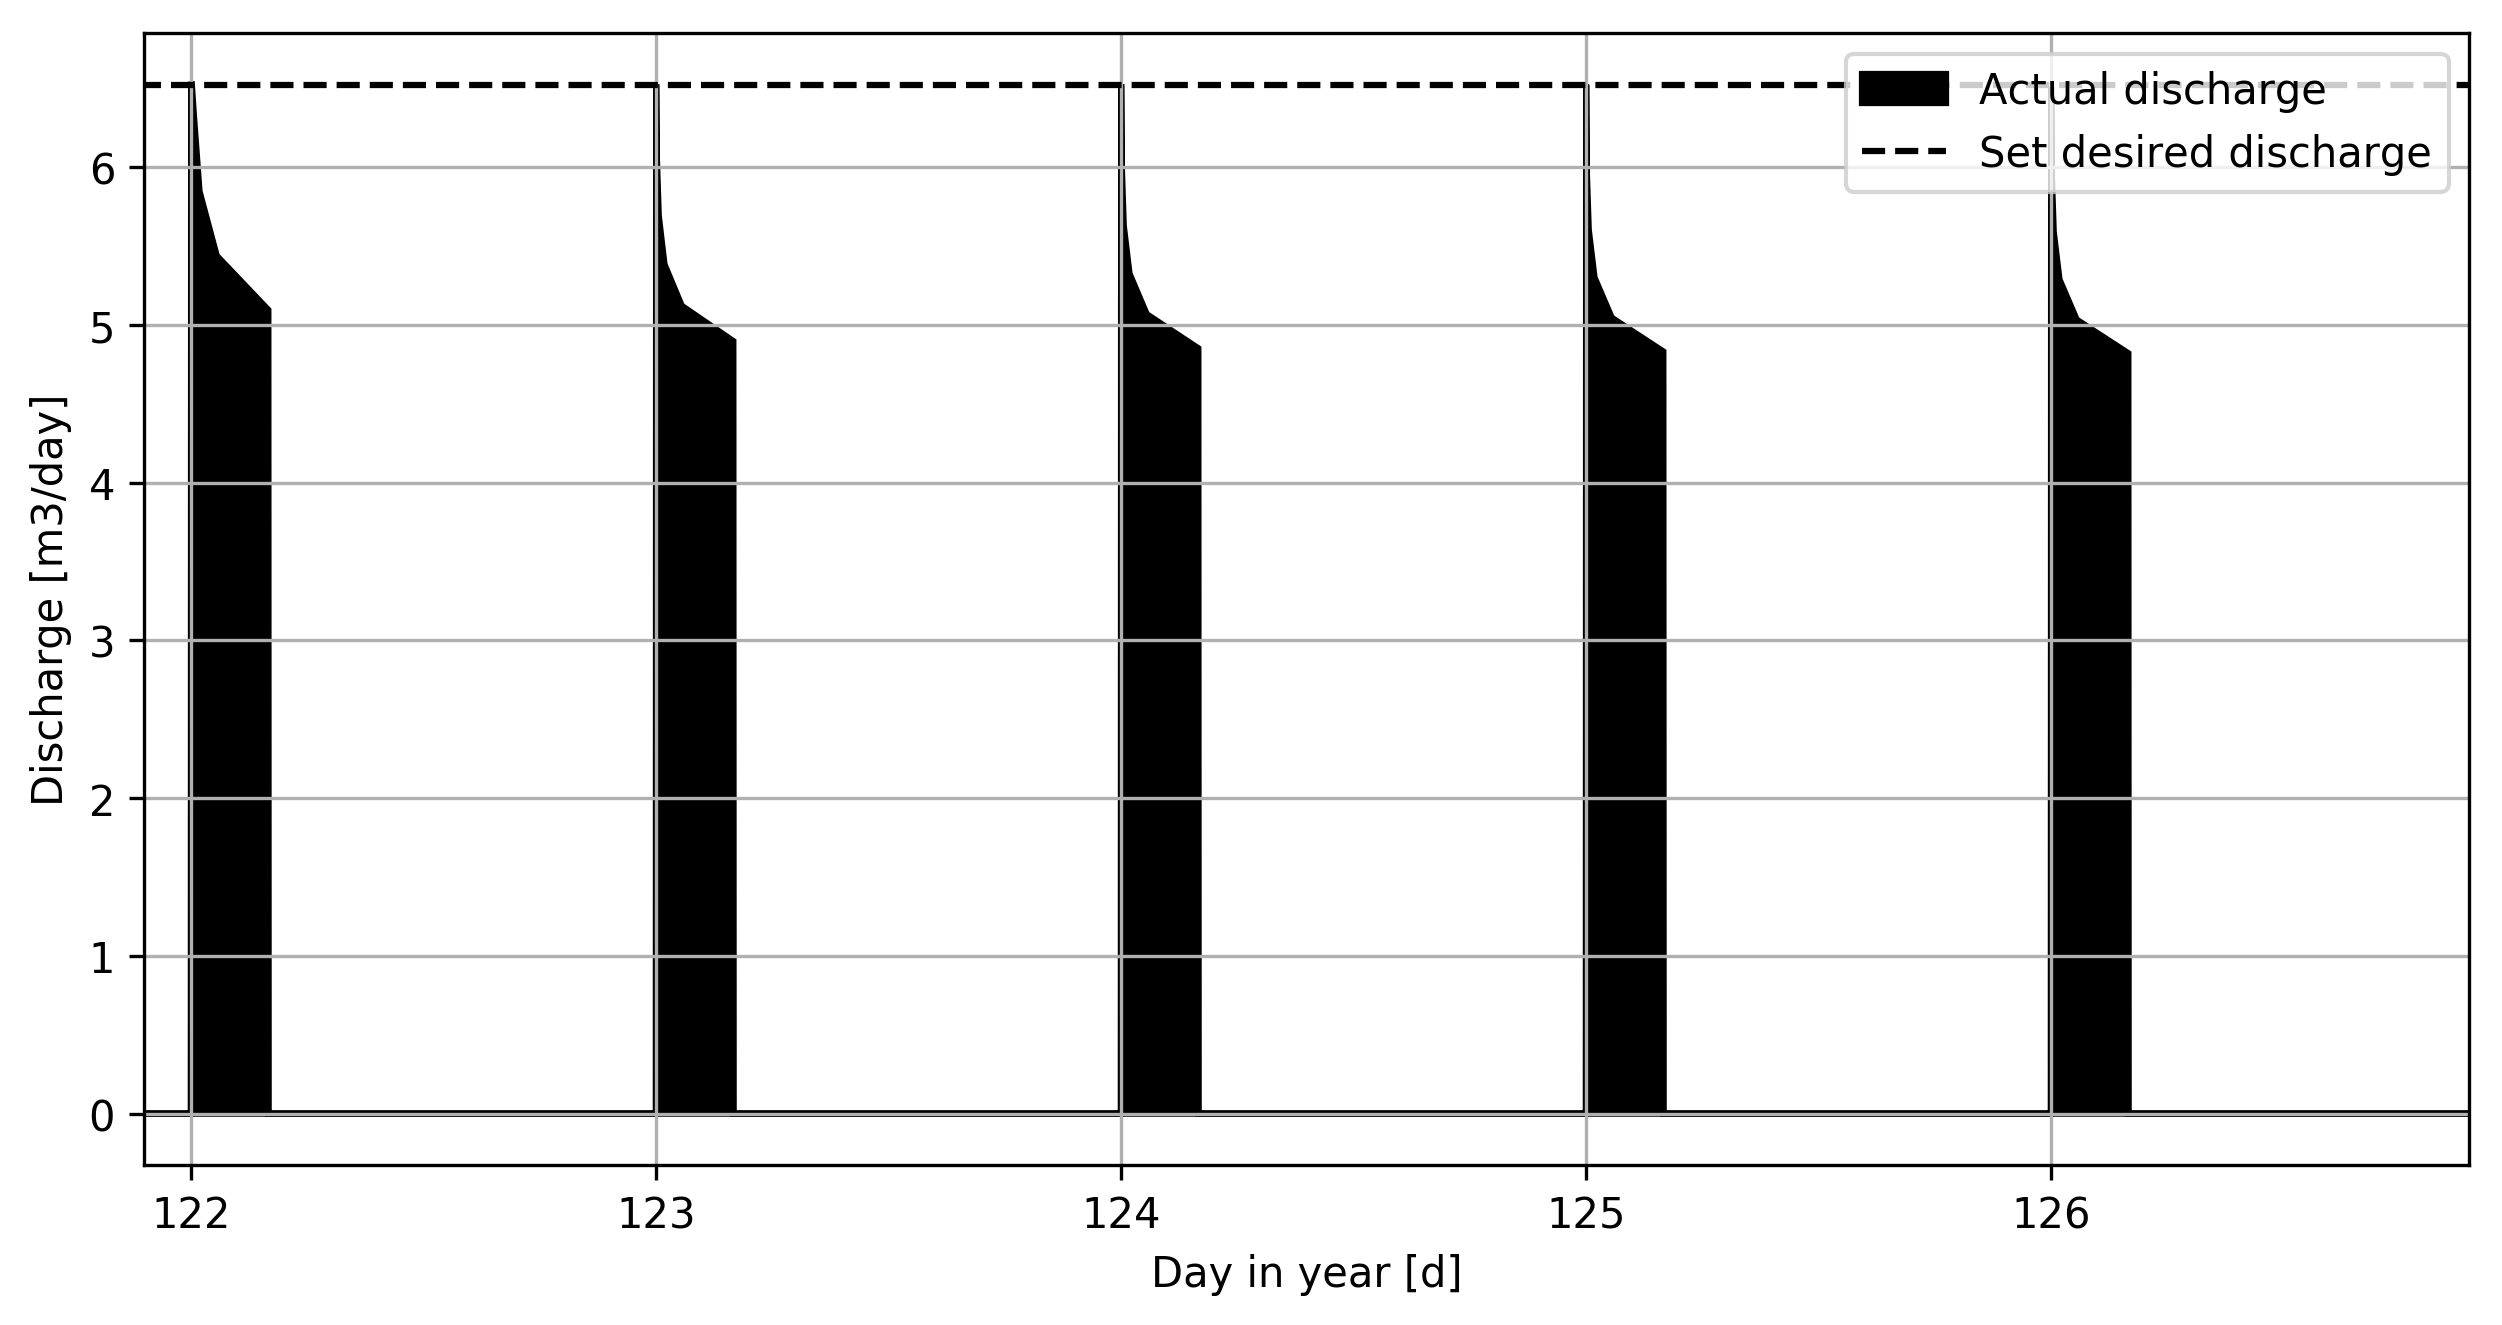
\includegraphics[width=\linewidth]{Sc1a1_Q122_126}
%		\captionsetup{justification=centering}		
%		\caption{\label{fig:Sc1a1_Q122_126}}
%		\end{subfigure}\hfill
%	\begin{subfigure}[b]{0.5\linewidth}
%        \centering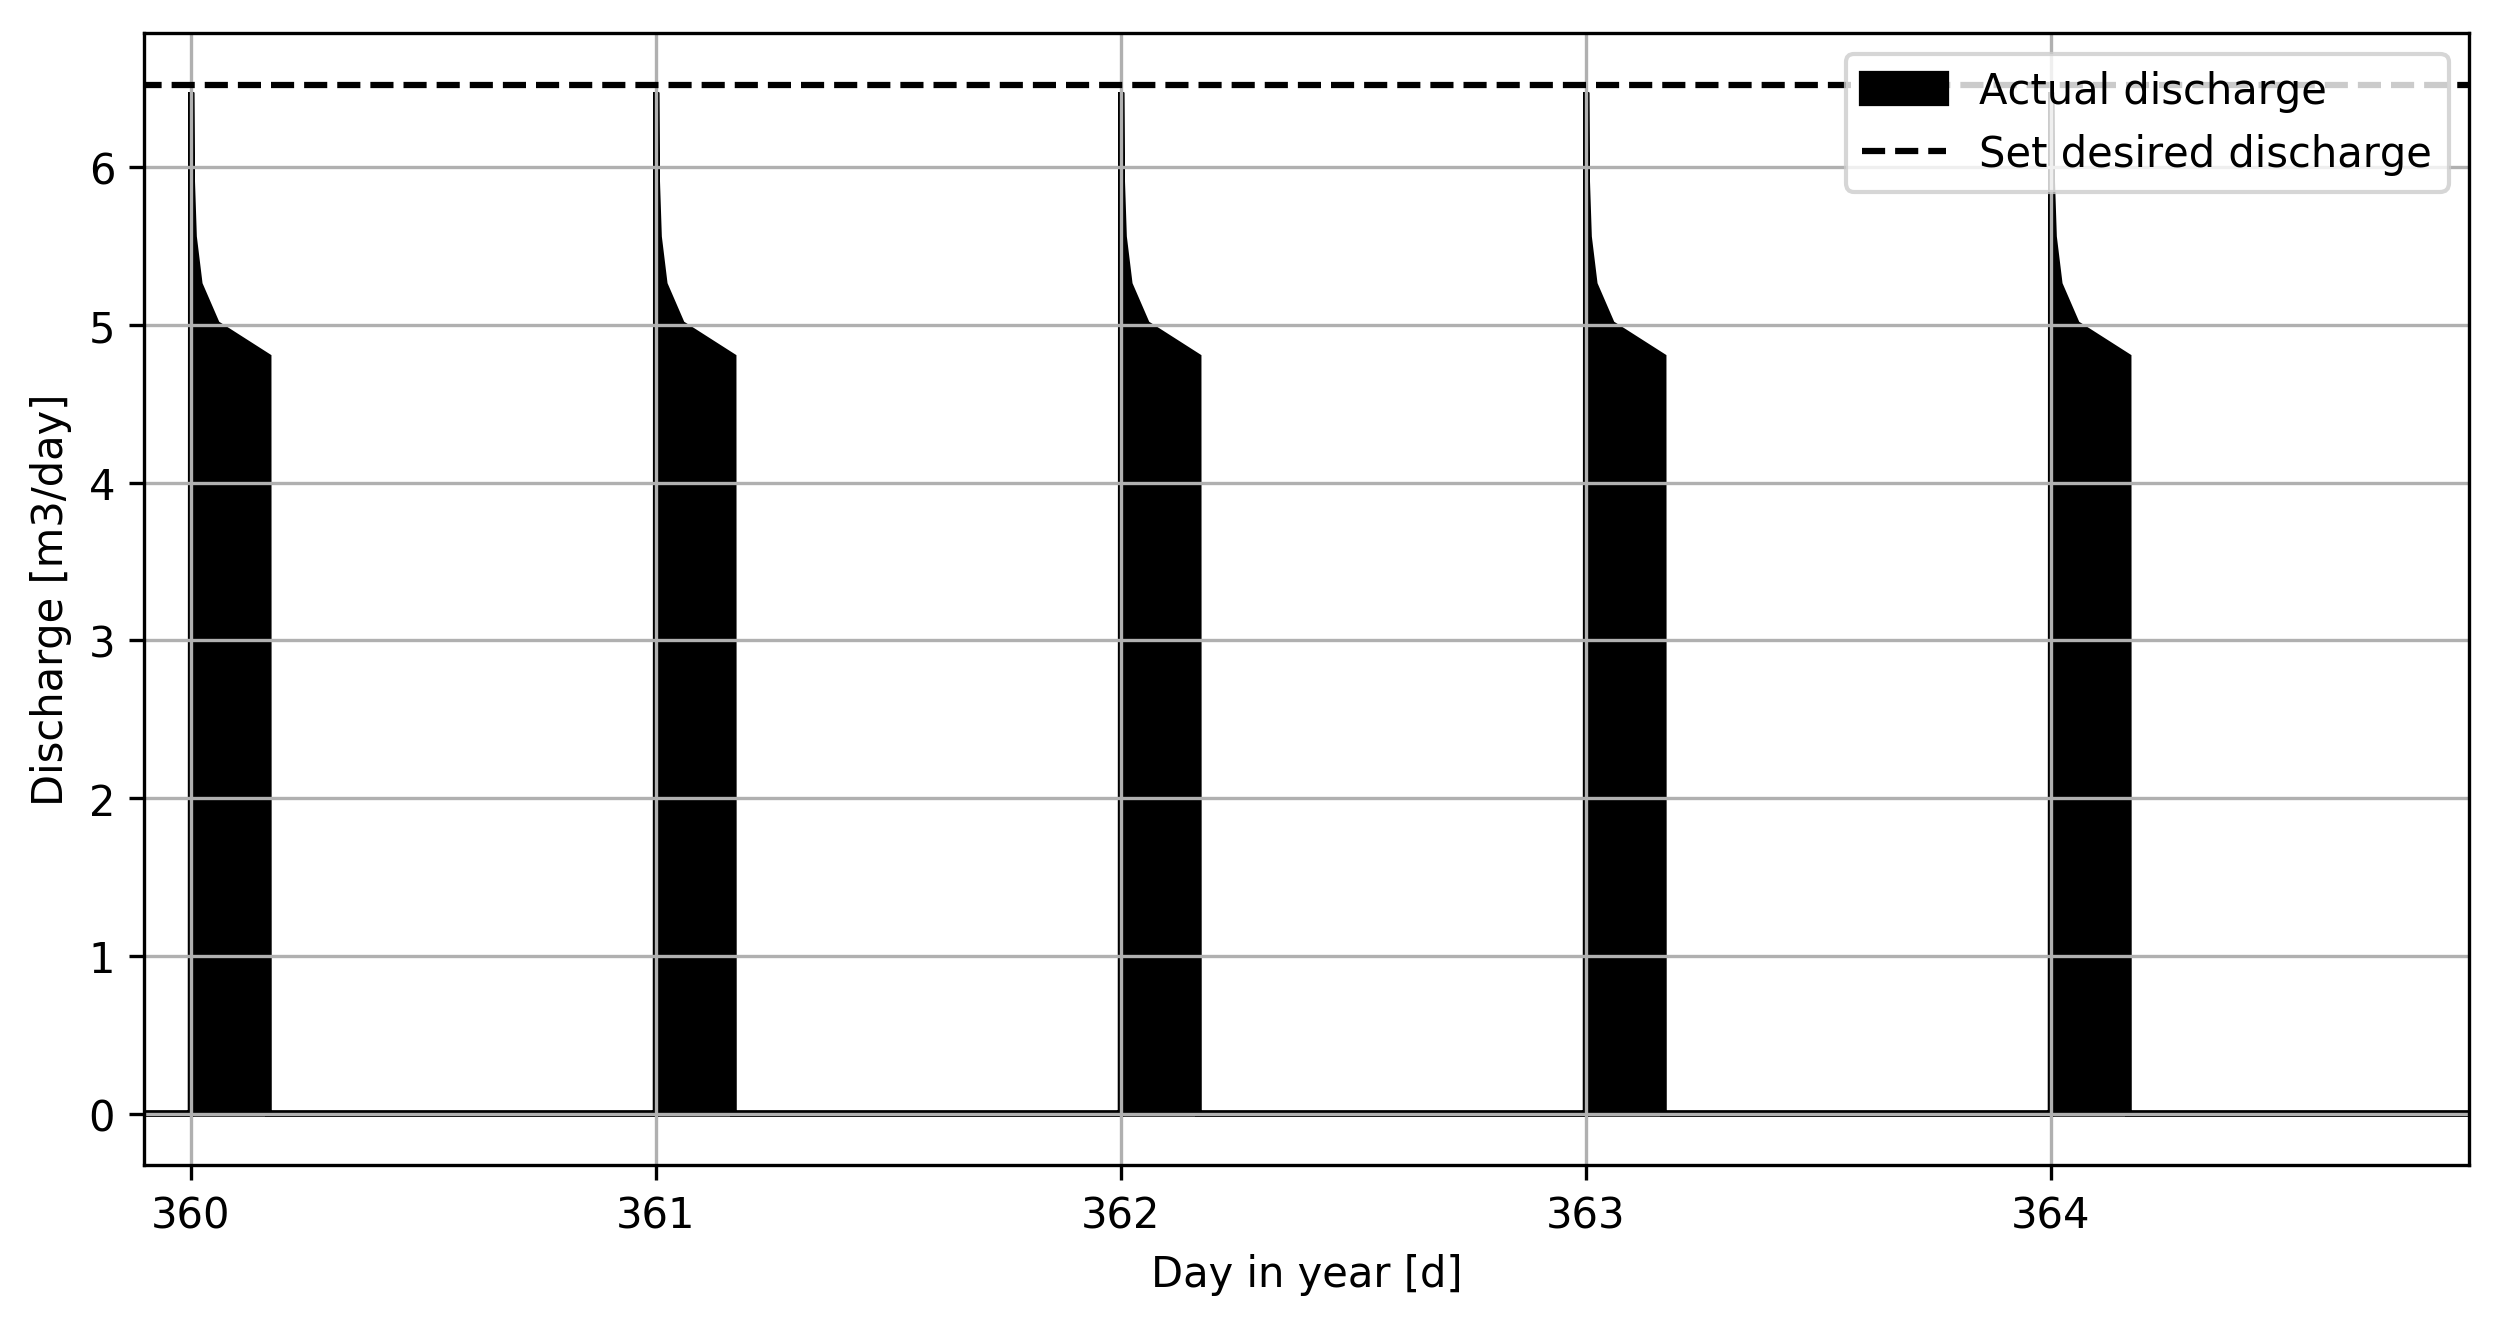
\includegraphics[width=\linewidth]{Sc1a1_Q360_364}
%		\captionsetup{justification=centering}		
%		\caption{\label{fig:Sc1a1_Q360_364}}
%		\end{subfigure}
%		\captionsetup{justification=centering}	
%	\caption{Example scenario 1 - base model - Discharge performance for (\subref{fig:Sc1a1_Q122_126}) the first five days and (\subref{fig:Sc1a1_Q360_364}) the last five days of dry season} 
%	\label{fig:Example_Sc1_base_discharge}
%\end{figure} 
%
%\begin{figure}[H]
%	\centering
%	\begin{subfigure}[b]{0.5\linewidth}
%		\centering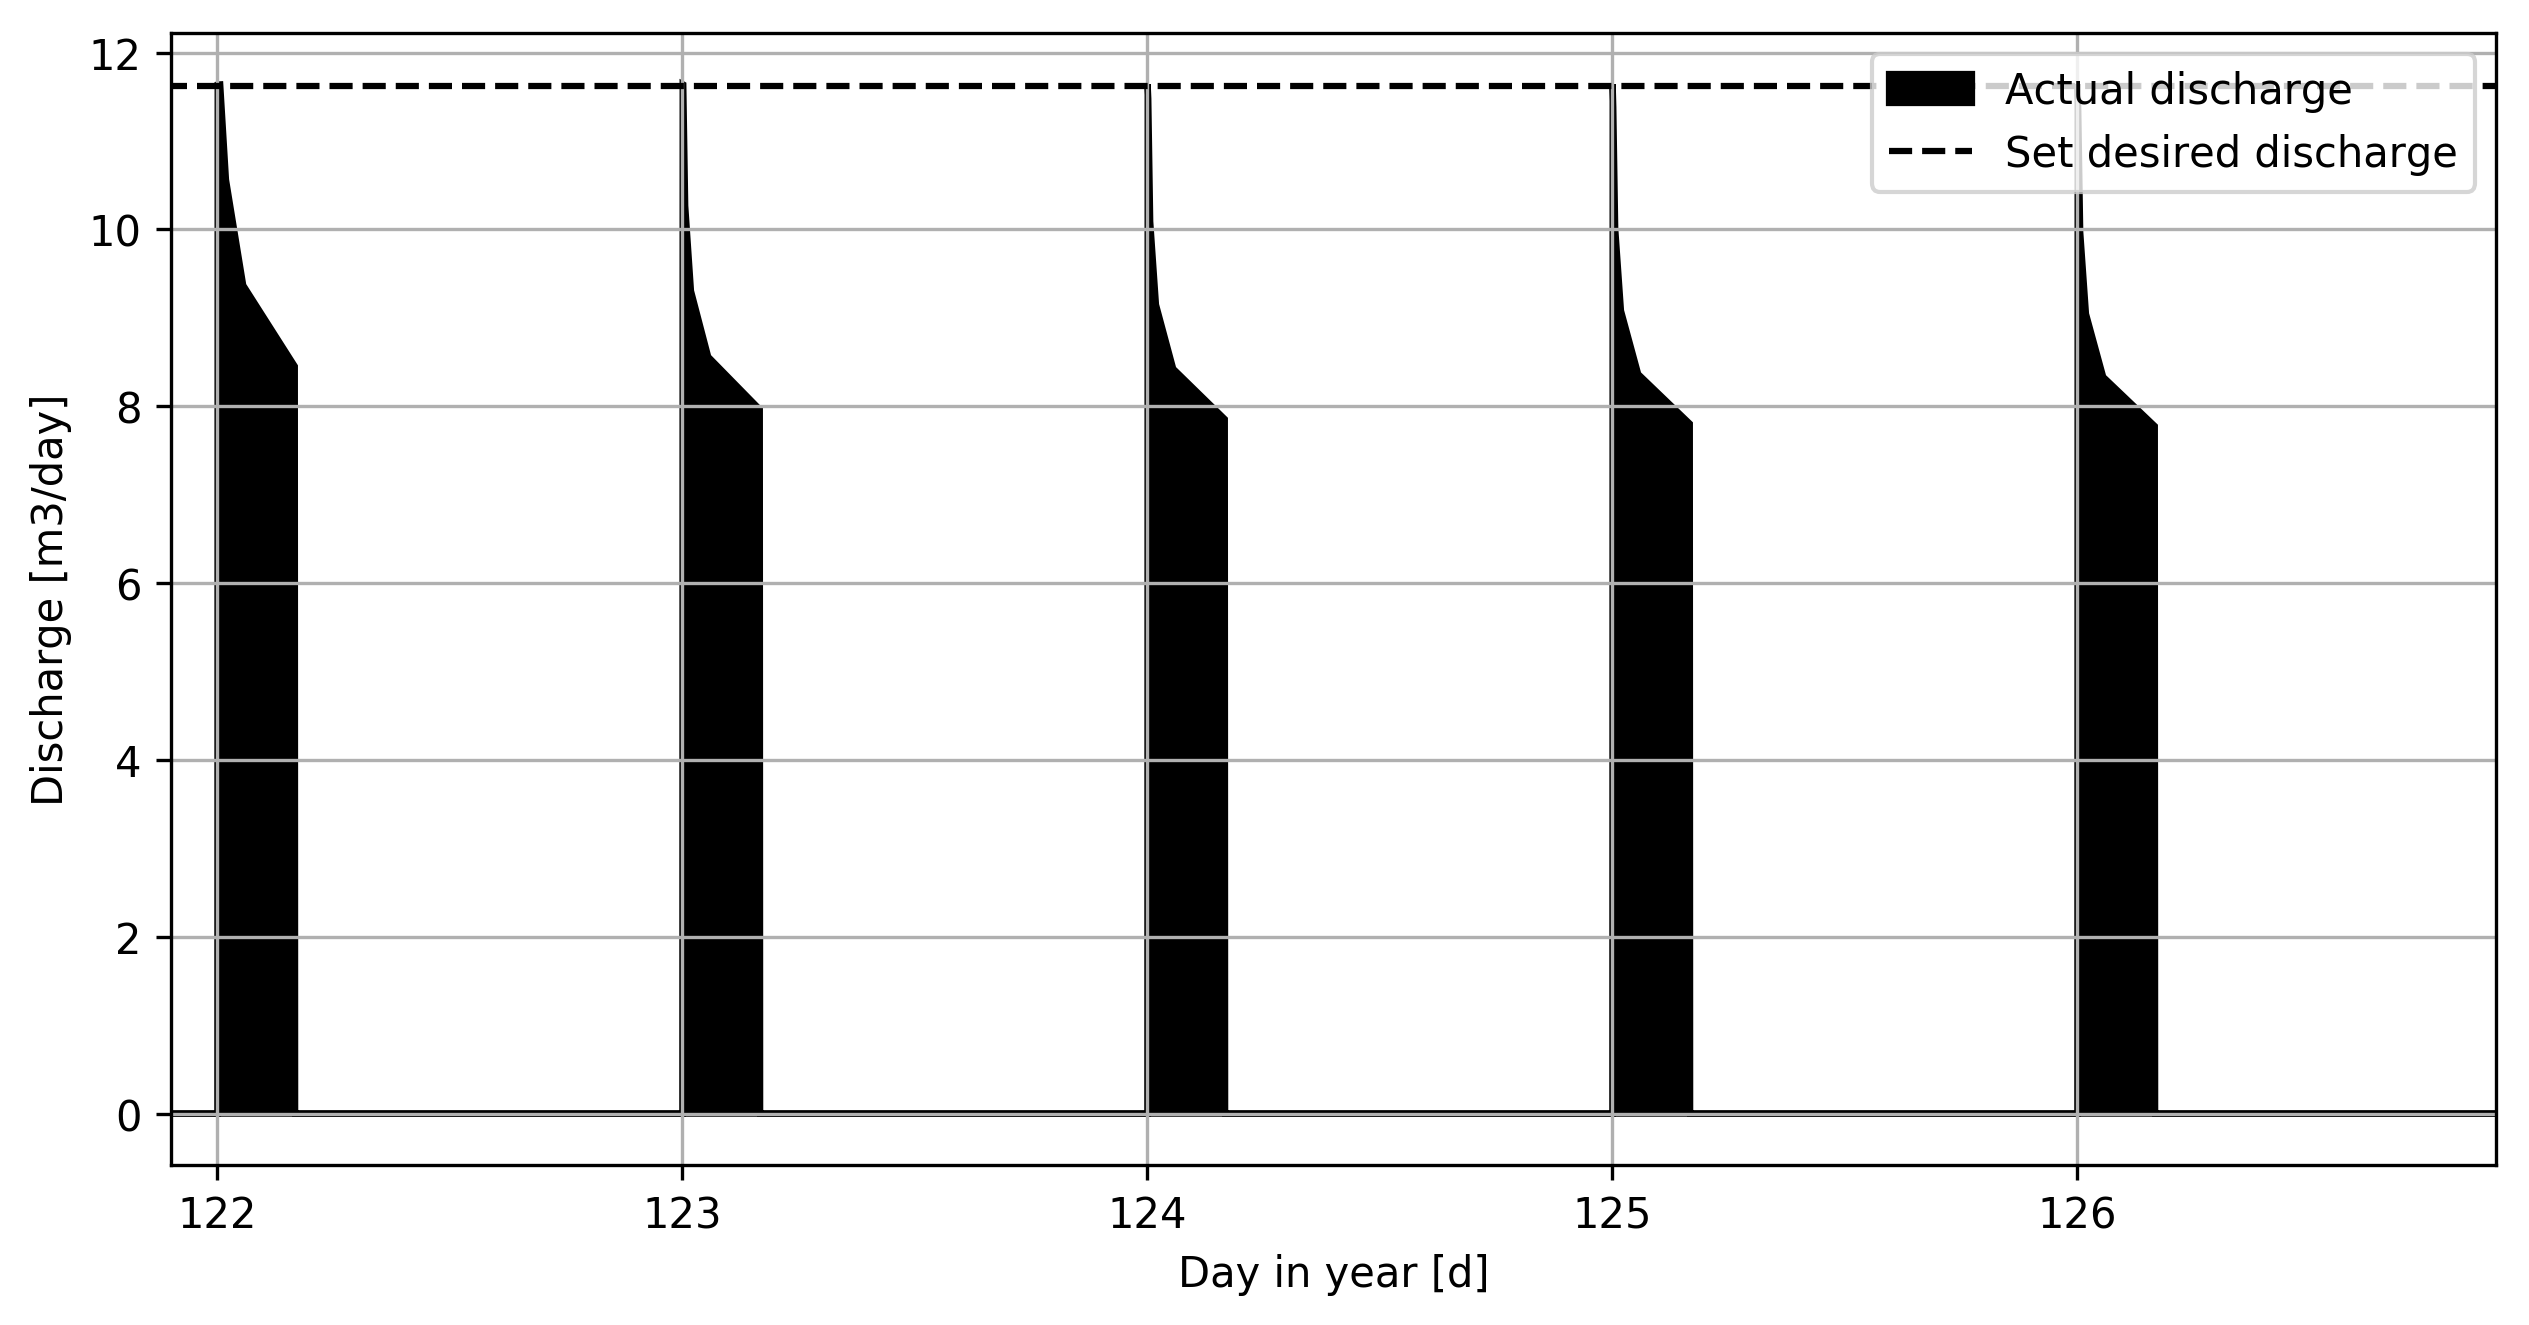
\includegraphics[width=\linewidth]{Sc1a5_Q122_126}
%		\captionsetup{justification=centering}		
%		\caption{\label{fig:Sc1a5_Q122_126}}
%		\end{subfigure}\hfill
%	\begin{subfigure}[b]{0.5\linewidth}
%        \centering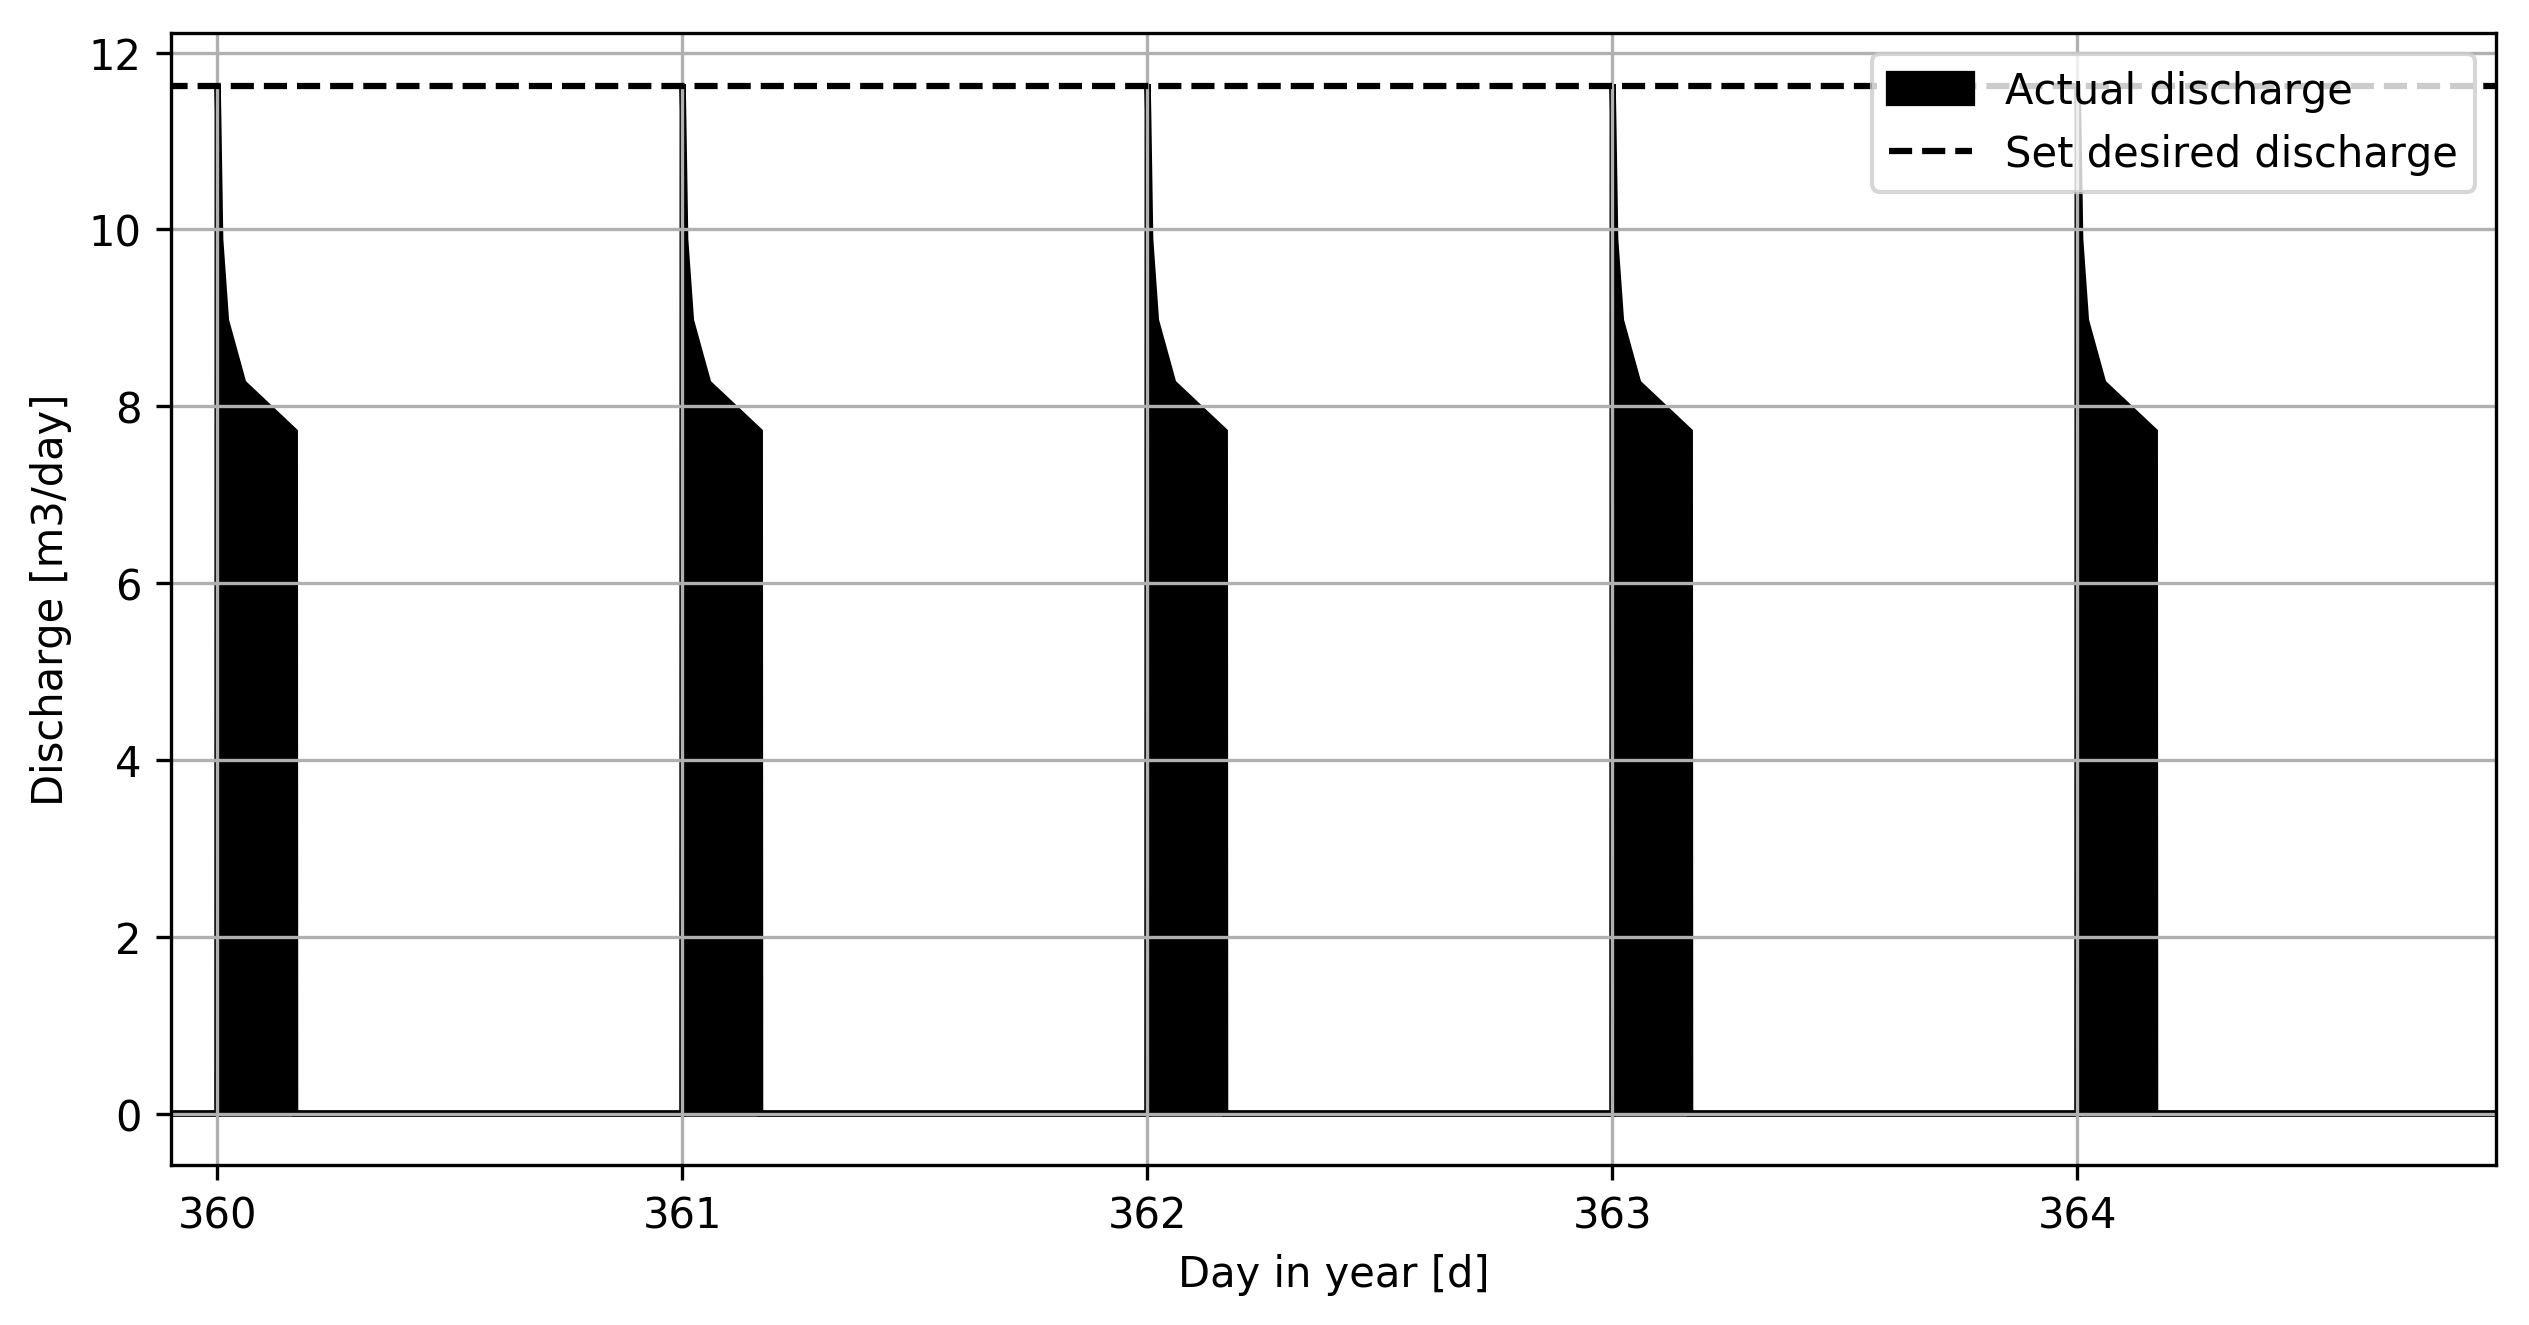
\includegraphics[width=\linewidth]{Sc1a5_Q360_364}
%		\captionsetup{justification=centering}		
%		\caption{\label{fig:Sc1a5_Q360_364}}
%		\end{subfigure}
%		\captionsetup{justification=centering}	
%	\caption{Example scenario 1 - 5x base model well diameter - Discharge performance for (\subref{fig:Sc1a5_Q122_126}) the first five days and (\subref{fig:Sc1a5_Q360_364}) the last five days of dry season} 
%	\label{fig:Example_Sc1_5x_diam_discharge}
%\end{figure} 

\subsection{Reduction of well skin resistance}
\label{subsec:Up_well_res}
This type of improvement is characterised by its applicability on existing ASR systems. Fieldwork showed, some already installed systems performed better than others. If the right cleaning equipment is present, a reduction of well skin resistance can potentially offer solutions. Based on the statements done by \citet{LeonardF.KonikowGeorgeZ.HornbergerKeithJ.Halford2009} and \citet{Houben2015}, the base model is designed with a gavel-pack that is moderately permeable. The (simulated) improvements are implemented by a stepwise increase of the the gravel-pack hydraulic conductivity. As visible in Figure \ref{fig:Schematic_up_well_res}, gravel-pack hydraulic conductivities that exceed the soil (scenario dependent) hydraulic conductivities are considered. 

%In northern Ghana, multiple ASR systems are already installed. 
%duction of the well skin resistance can be applied on existing ASR systems. If appropriate equipment is present, Since , this type of improvements is of interest.
%
%making this type of improvement of extra interest.  are already installed, multiple ASR systems are present in northern Ghana  currently  This type of improvement 
%The well skin hydraulic conductivity is typically lower than the original aquifer hydraulic conductivity ($K_{h}$)  \citep{LeonardF.KonikowGeorgeZ.HornbergerKeithJ.Halford2009,Houben2015}. A base model well skin hydraulic conductivity that equal 1/5 of the aquifer hydraulic conductivity is assumed. The definition of the well skin resistance is detailed described in Appendix \ref{chapter:Extense_Modflow_model}.)
%

\begin{figure}[H]
\centering
\begin{tikzpicture}
\node [mybox] (box){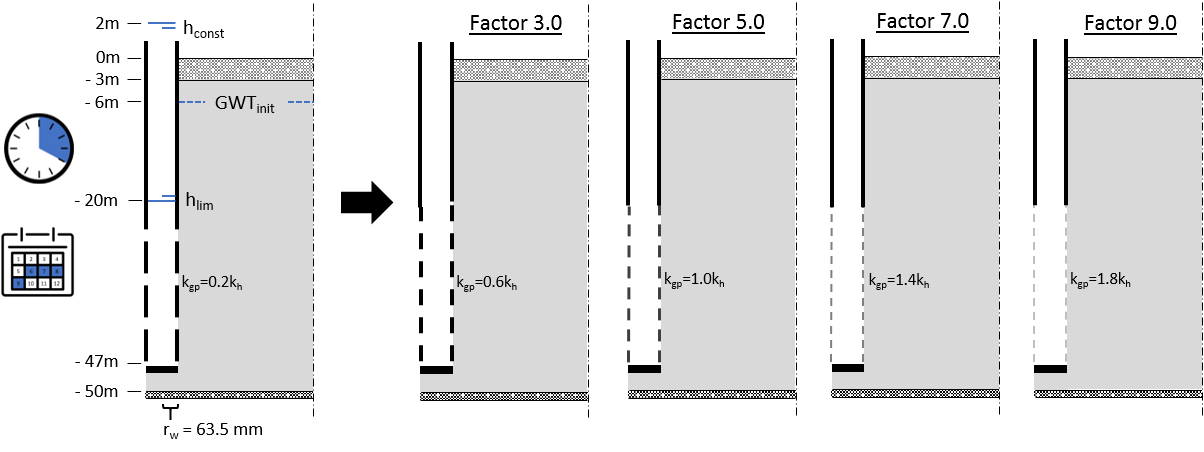
\includegraphics[width=0.9\linewidth]{Schematic_up_well_res}};  
\node[title, right=10pt] at (box.north west) {Schematic reduction well skin resistance};
\end{tikzpicture}
\captionsetup{justification=centering}
\caption{Schematic reduction well skin resistance}
\label{fig:Schematic_up_well_res}
\end{figure}

Figure \ref{fig:Results_up_well_res} presents the results of the (simulated) improvement of an ASR system by the modification of the gravel-pack hydraulic conductivity. It can be seen that the ASR system performance (on total recharge, discharge and Recovery ratio) increases by improved gravel-pack permeabilities. A non-linear ascending relation is present. In the scope of this research (upto nine times the base model gravel-pack permeability) in- and outflow volumes of approximately two times the original values are achieved. Significant improvements can be made, especially in the lower interval of well permeabilities. In the contrary, system degradation in skin performance can be devastating. 

\begin{figure}[h!]
 \centering
 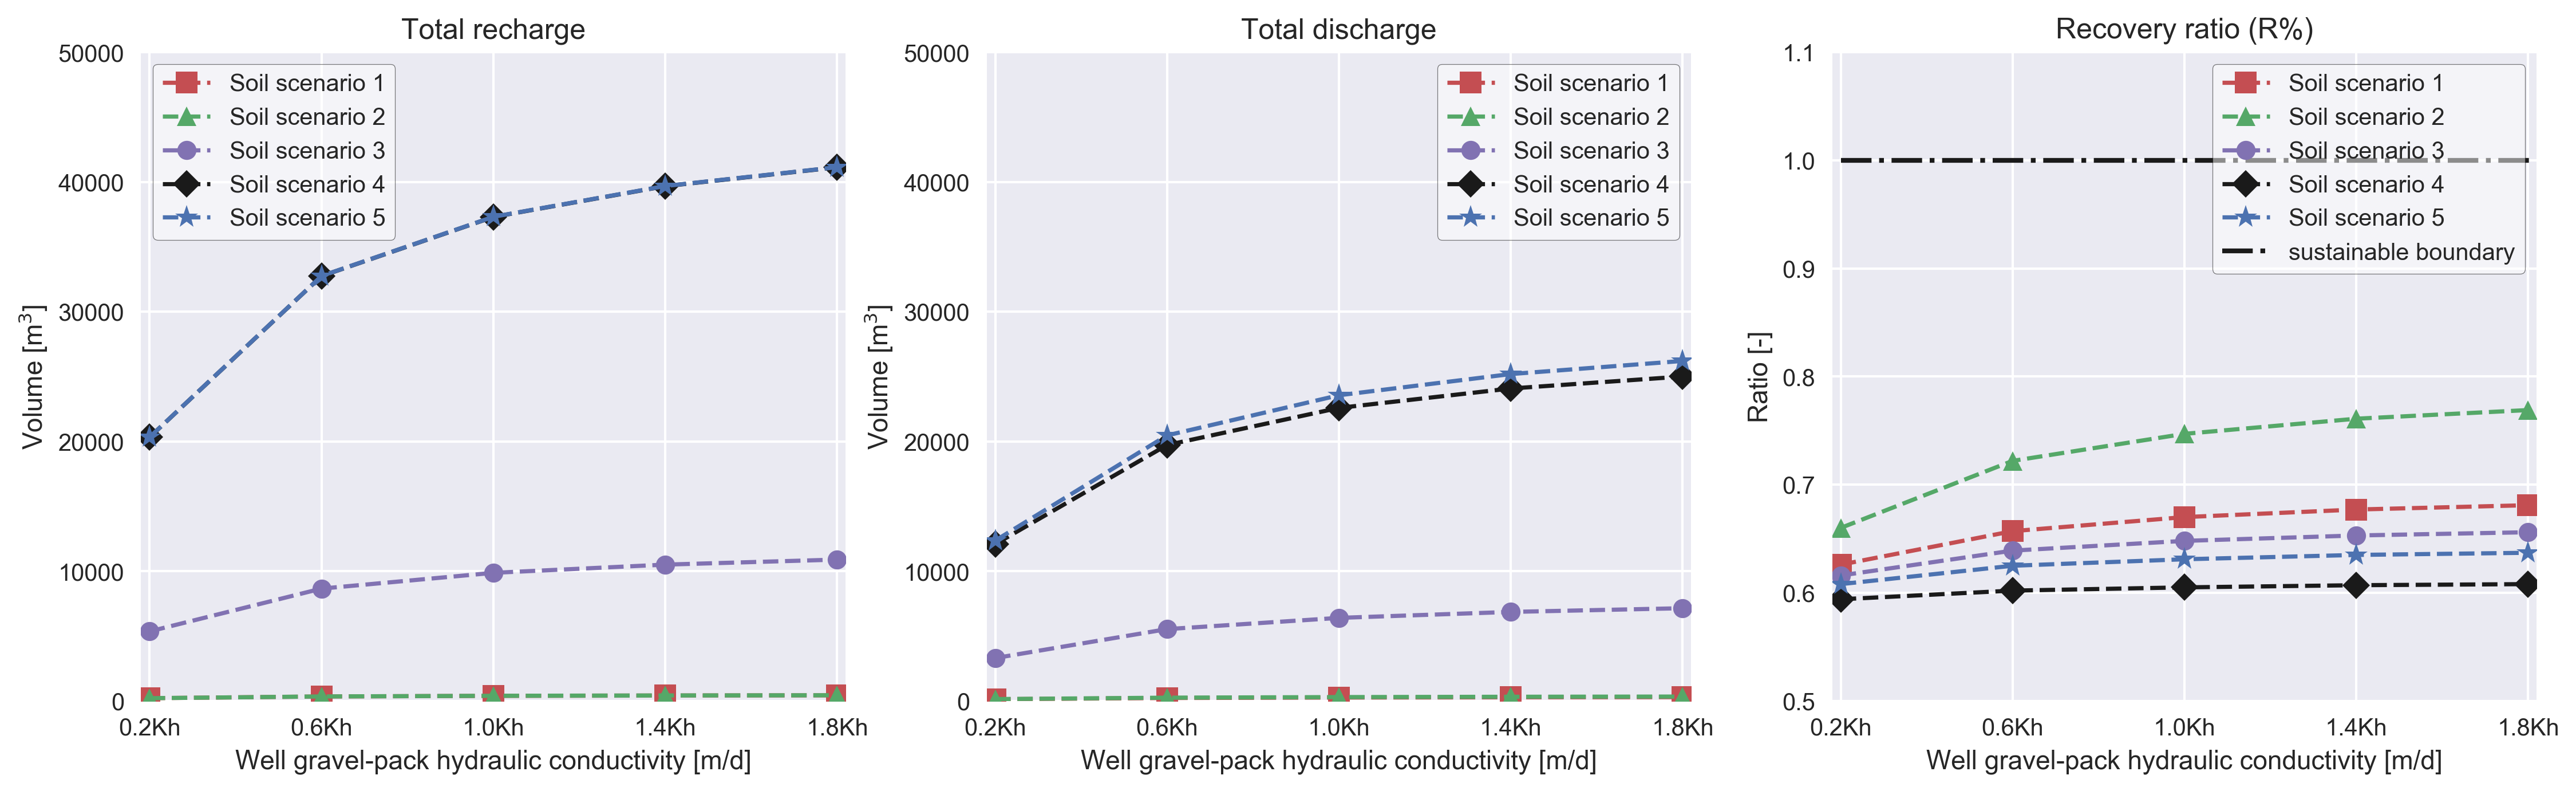
\includegraphics[width=1.0\linewidth]{Results_up_well_res}
 \captionsetup{justification=centering} 
 \caption{Results of yearly total volumes (in, out, ratio) by reduction well skin resistance}
 \label{fig:Results_up_well_res}
\end{figure}

* Note, although not clearly visible (especially, when total recharge volumes are taken into account) all soil scenarios are included in the presented figures.  \\

%
%\subsection{Cleaning of borehole depth}
%\label{subsec:Up_clean}
%Unlike the previous forms of upscaling, upscaling by system cleaning does not use the base model scenarios as reference start. All prior simulations are based on the assumption of a clean system. Fieldwork inspection showed clean systems are absent in nature. Debris accumulates at the borehole bottom. Direct consequence is a decrease in well penetration length. By the approach of a stepwise increase (5 steps) in borehole depth, the cleaning of a clogged borehole is simulated (\ref{fig:Schematic_up_clean}).   
%
%\begin{figure}[h!]
%\centering
%\begin{tikzpicture}
%\node [mybox] (box){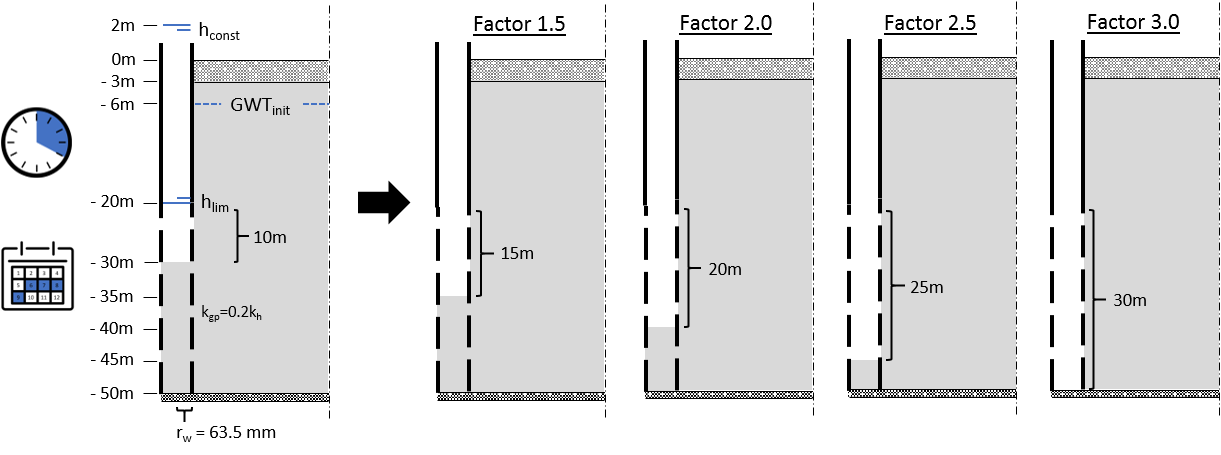
\includegraphics[width=0.9\linewidth]{Schematic_up_clean}};  
%\node[title, right=10pt] at (box.north west) {Schematic cleaning borehole depth};
%\end{tikzpicture}
%\captionsetup{justification=centering}
%\caption{Schematic cleaning borehole depth}
%\label{fig:Schematic_up_clean}
%\end{figure}
%
%System cleaning has a positive impact on both the wet season recharge and dry season discharge. Total volumes infiltrated and withdrawn are approximately linear dependent on the (clean) well screen length. Effects of non-uniform flow (partially aguifer penetration) are not of significance for the simulation conditions applied in this study.  
%
%\begin{figure}[h!]
% \centering
% 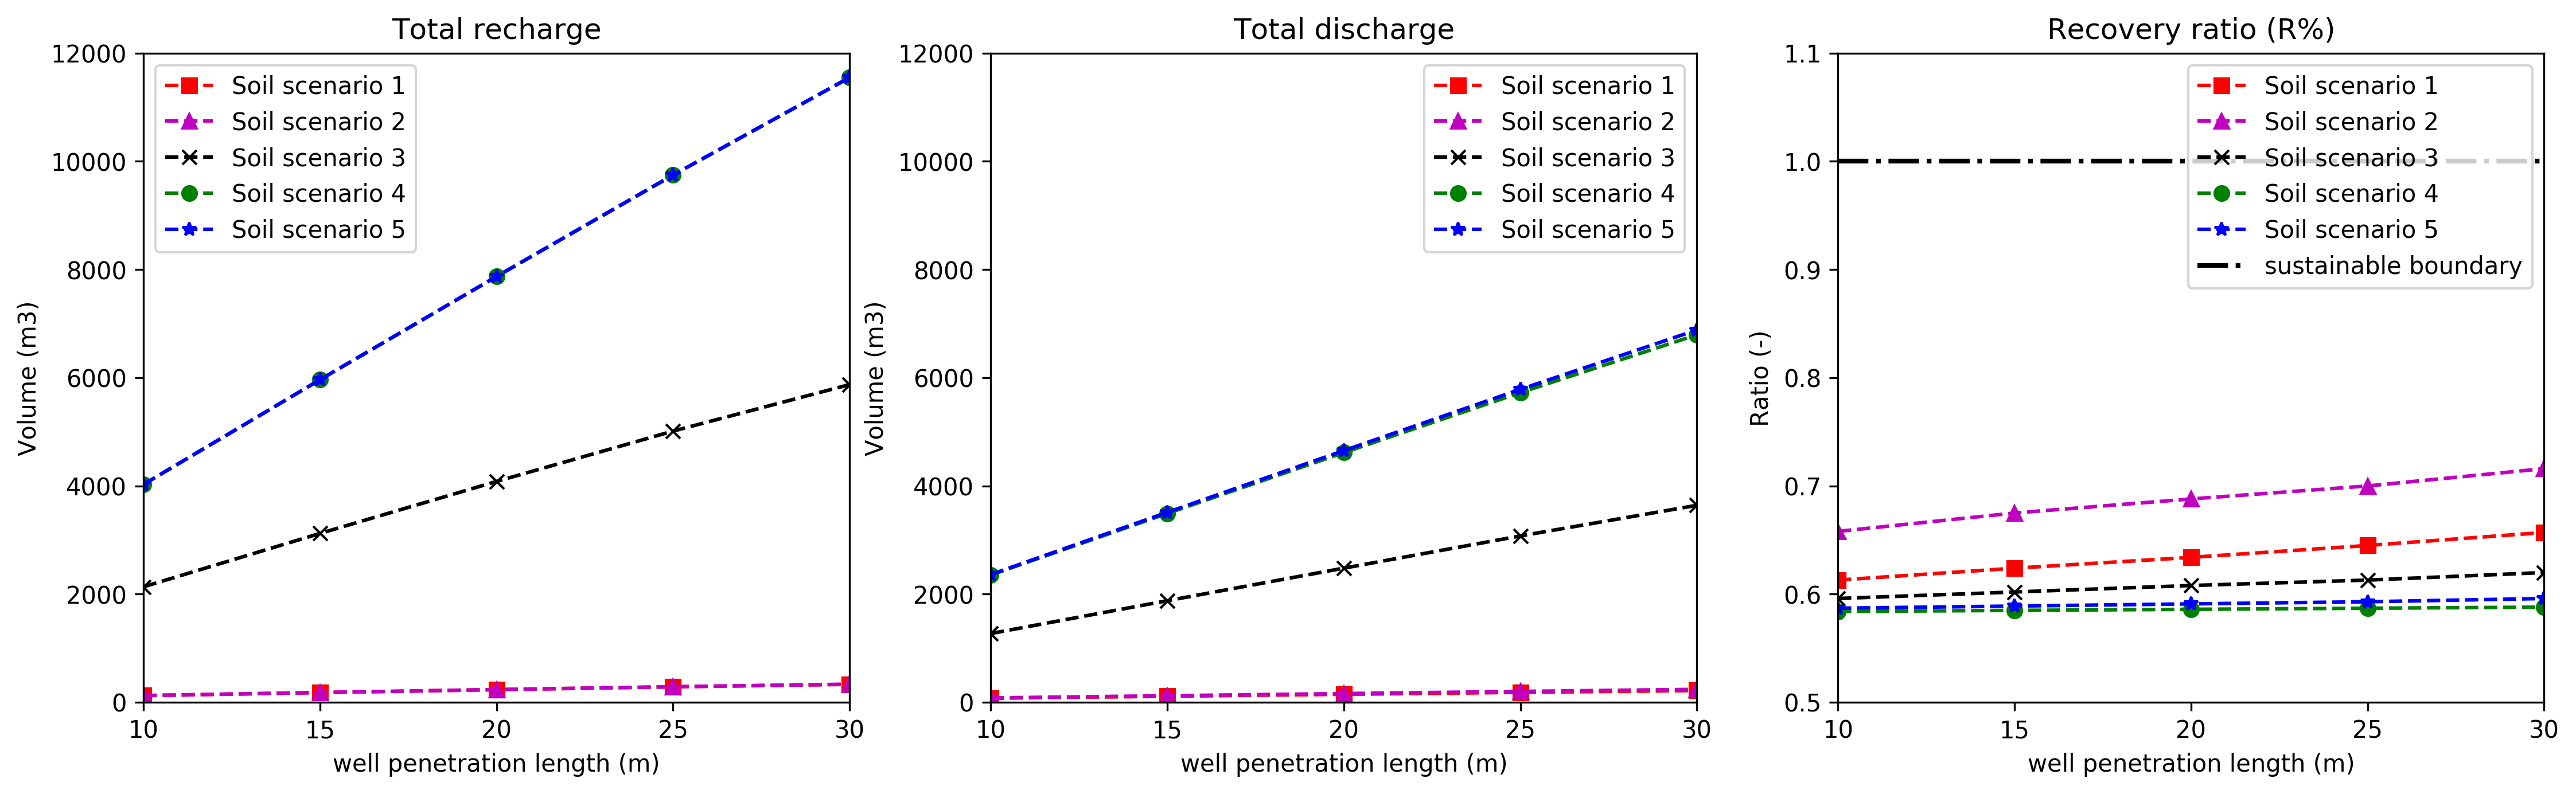
\includegraphics[width=1.0\linewidth]{Results_up_clean}
% \captionsetup{justification=centering} 
% \caption{Results of yearly total volumes (in, out, ratio) by cleaning the borehole depth}
% \label{fig:Results_up_clean}
%\end{figure}
%
%System cleaning ensures a increase in recovery ratios (for all soil scenarios). In an absolute sense the total volumes discharged are slightly more affected by cleaning compared to recharged volumes. In general recovery ratio increase is not significant. Moreover the ratios stay within the range of sustainable use. Deepening the borehole (to its original length) improves system operation. Cleaning of (partially) clogged systems is advisable. 

\section{ASR system sensitivity}
\label{section:sens_analysis}
The performance of an ASR system is dependent on the natural circumstances of its surroundings. This section explores the impact of changing natural conditions on the system performance. The system sensitivity is expressed by the test criteria: total recharge, discharge and Recovery ratio ($R_{\%}$).

\subsection{Degradation of well depth by clogging}
\label{subsec:Sens_well_depth}
Prior simulations (Section \ref{section:Base_model_perf} - \ref{section:ASR_upscaling}) are executed by the implementation of a borehole that is fully function in depth. Fieldwork inspection revealed that sand and/or clay can accumulate at the borehole bottom. The presence of debris can reduce the well penetration depth. By a decrease in model screen length, the borehole clogging of an ASR system is simulated (\ref{fig:Schematic_up_clean_reverse}). In four successive steps the 30 m screen length of an already partially penetrating well is reduced to a minimum of 10 m. 

\begin{figure}[H]
\centering
\begin{tikzpicture}
\node [mybox] (box){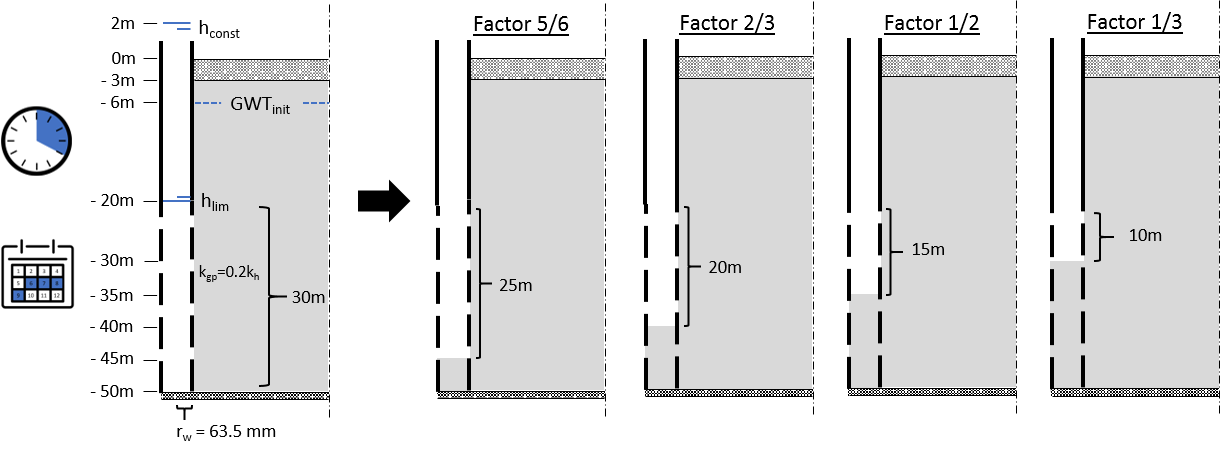
\includegraphics[width=0.9\linewidth]{Schematic_up_clean_reverse}};  
\node[title, right=10pt] at (box.north west) {Schematic degradation well depth by clogging};
\end{tikzpicture}
\captionsetup{justification=centering}
\caption{Schematic degradation well depth by clogging}
\label{fig:Schematic_up_clean_reverse}
\end{figure}

The data in Figure \ref{fig:Results_up_clean_reverse} shows the system performance while the borehole screen length is stepwise reduced. Under the defined model condition (e.g. homogeneous aquifer), the observed relation between the active screen length and the test criteria (recharge, discharge and Recovery ratios) is close to (but not precisely) linear. In relative perspective, the average specific recharge and discharge volumes (m$^3$/m screen) increase while the length of well penetration is reduced. As stated in Table \ref{tab:sc3_up_clean_rev_specific_volume}, this increase is not significant. Moreover, the total inflow and outflow volumes are increasingly negative affected by a further reduction of the well screen length (Table \ref{tab:sc3_up_clean_rev_specific_volume_reduction}). The preservation of maximum borehole depth should be pursued, to obtain highest system functionalities. This can be achieved by the (preventive) use of a 'pulse drill'. 

\begin{figure}[H]
 \centering
 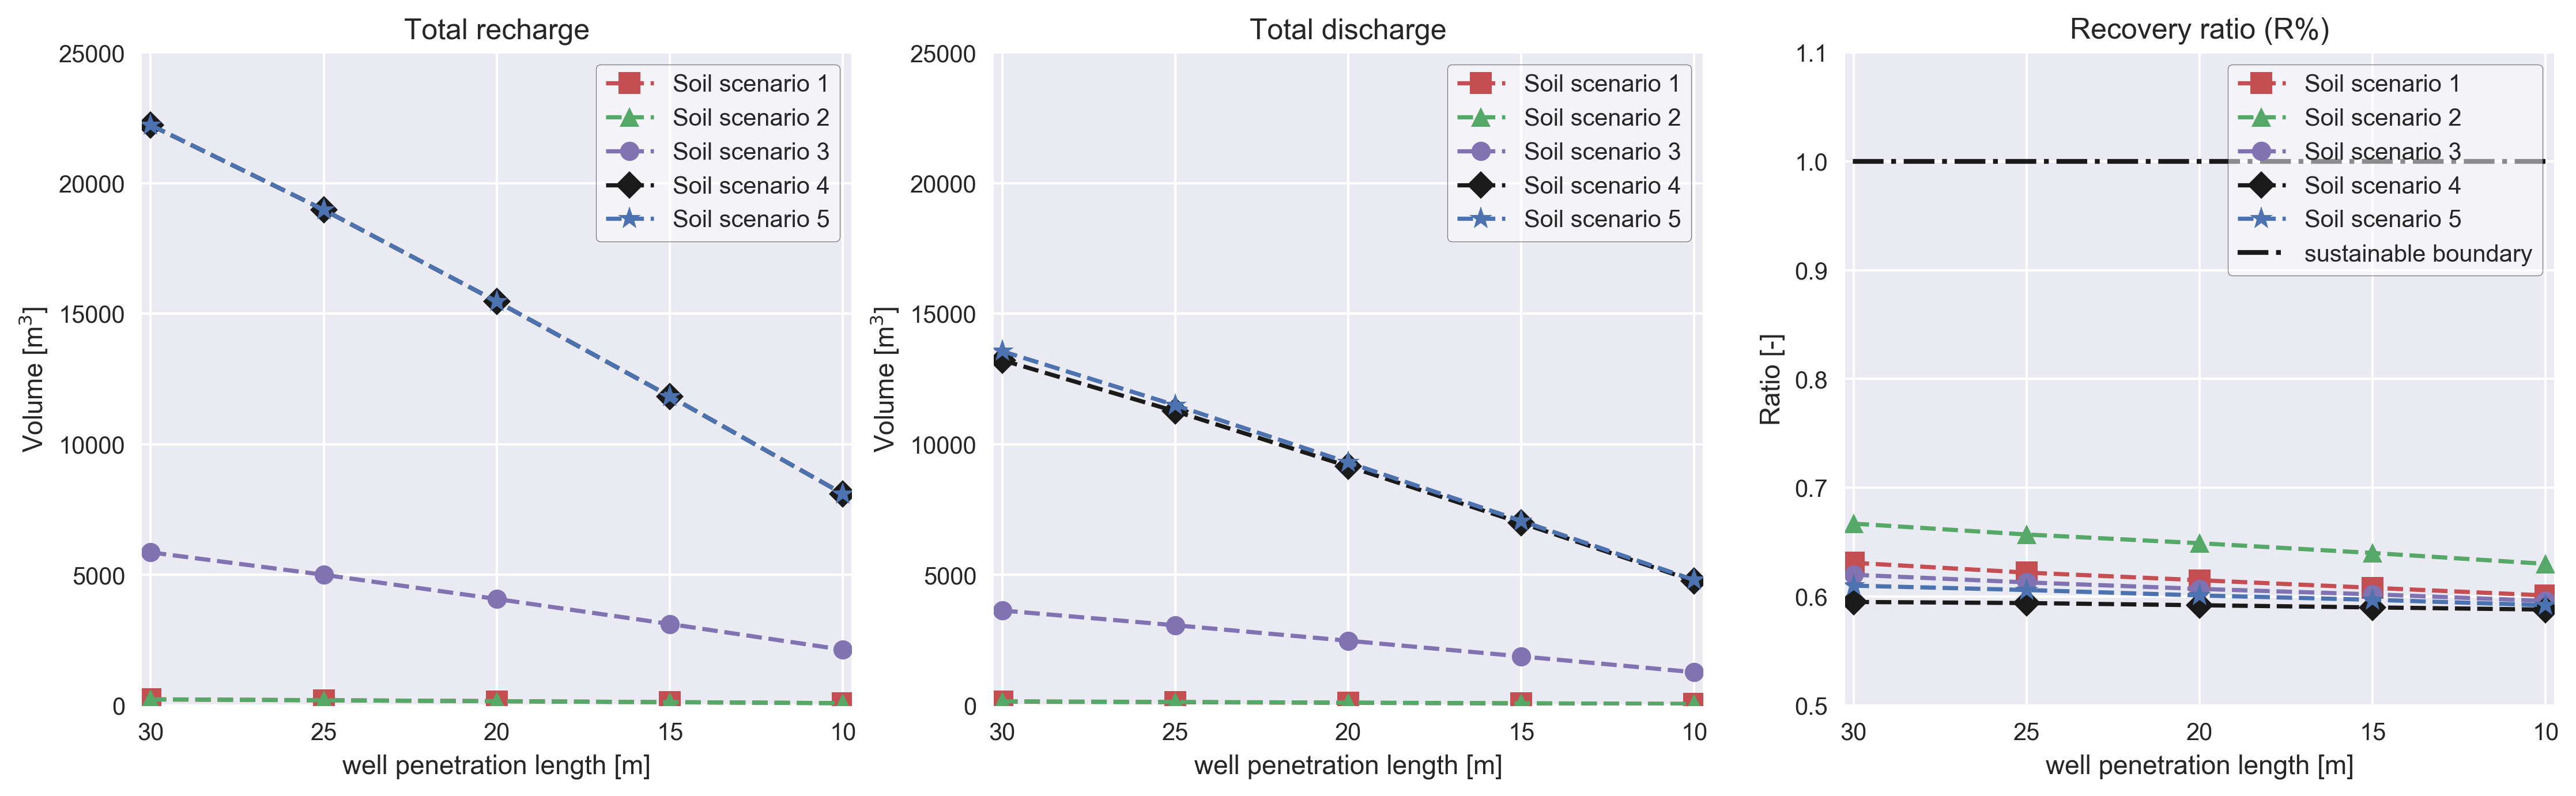
\includegraphics[width=1.0\linewidth]{Results_up_clean_reverse}
 \captionsetup{justification=centering} 
 \caption{Results of yearly total volumes (in, out, ratio) by degradation well depth}
 \label{fig:Results_up_clean_reverse}
\end{figure}

As an example, a more precise distribution of the soil scenario 3 recharge volumes over the (variable) well screen length is presented in Figure \ref{fig:Sc3c_recharge_layers} (Appendix \ref{chapter:MODFLOW_additional}). 

\subsection{Shortening wet season inundation time-span}
\label{subsec:Sens_del_t}
Within northern Ghana the duration of the wet season is spatially dependent. At higher latitudes the wet season time-span is generally less than four months \citep{HAP2011}. Besides, wet season duration differs annually. The relation between the wet season duration and the ASR system performance is described in this part of the sensitivity analysis. Through the application of three steps the synthetic base model flood duration (four months: June-September) is reduced. In successive order, the following shortened wet seasons are simulated: July-September, July-August and August.  
   
\begin{figure}[H]
\centering
\begin{tikzpicture}
\node [mybox] (box){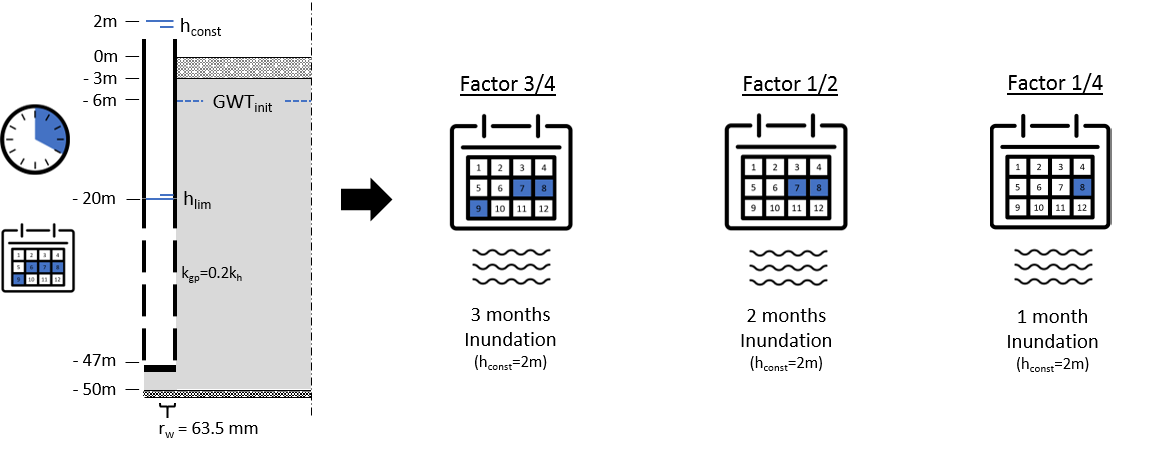
\includegraphics[width=0.9\linewidth]{Schematic_sens_del_t}};  
\node[title, right=10pt] at (box.north west) {Schematic shortening wet season inundation time-span};
\end{tikzpicture}
\captionsetup{justification=centering}
\caption{Schematic shortening wet season inundation time-span}
\label{fig:Schematic_sens_del_t}
\end{figure}

The data in Figure \ref{fig:Results_sens_del_t} shows an approximately linear relation. A fractional reduction of the (constant level) flood duration, causes an almost equal fractional decrease in the total volumes recharged. This ASR system performance can be explained by the fact that shortly after the inundation start (after approximately 5 days) the inflow rate is close to constant (but not steady) for as long as the research time-scope (four months). For each of the four time-span durations, the wet season performance is visualized in Figure \ref{fig:Sens_delt_Sc3_recharge_time} (Appendix \ref{section:addition_sens}). In the simulation, the desired discharge (dry season) is retained. Nonetheless, the obtained model discharges are affected in the situation of a flooding that lasts for two months (and less). A development caused by the predefined boundaries of sustainable system use (maximum allowed Recovery ratio of 100\%). 
 
\begin{figure}[h!]
 \centering
 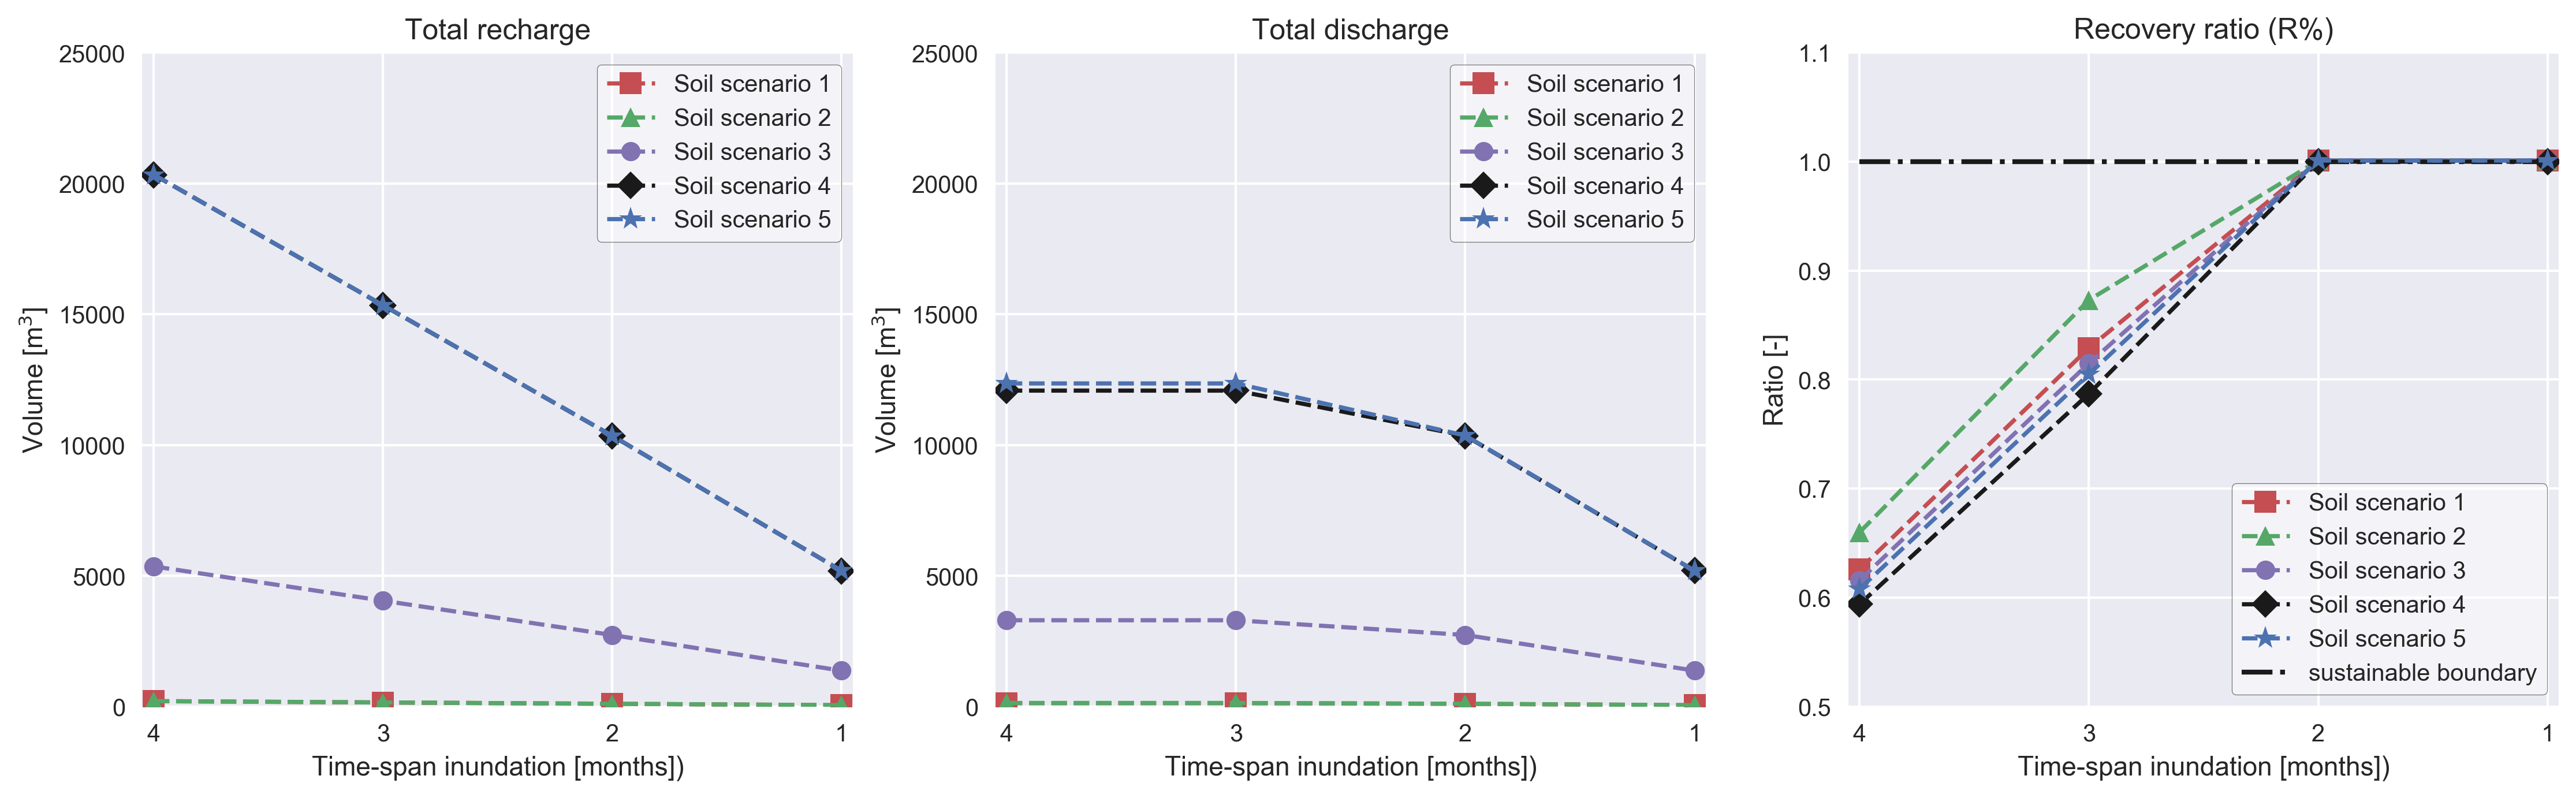
\includegraphics[width=1.0\linewidth]{Results_sens_del_t}
 \captionsetup{justification=centering} 
 \caption{Results of yearly total volumes (in, out, ratio) while shortening wet season inundation time-span}
 \label{fig:Results_sens_del_t}
\end{figure}

\subsection{Reduction wet season inundation level}
\label{subsec:Sens_del_h}
As mentioned by the \citet{HAP2011}, within northern Ghana the wet season is variable in terms of duration ánd intensity. Different flood levels are encountered by local inhabitants (Appendix \ref{chapter:fieldworkresults}). Moreover, the (initial) groundwater tables are not fixed. Based on fieldwork inspection it can be confirmed that the GWT in northern Ghana varies (Appendix \ref{chapter:fieldworkresults}). The impact of lower flood inundation levels is analysed in combination with increased initial groundwater tables. Relative to the base model ($\Delta h$ is 8m) the $\Delta h$ is reduced (in steps of 2 m) to a minimum of $\Delta h$ is 2 m.

\begin{figure}[H]
\centering
\begin{tikzpicture}
\node [mybox] (box){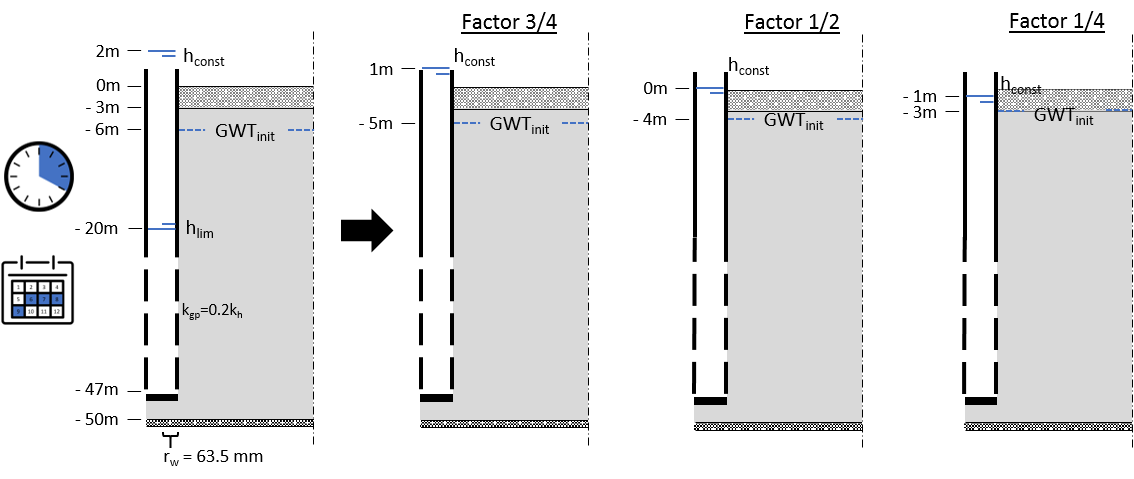
\includegraphics[width=0.9\linewidth]{Schematic_sens_del_h}};  
\node[title, right=10pt] at (box.north west) {Schematic reduction wet season inundation level};
\end{tikzpicture}
\captionsetup{justification=centering}
\caption{Schematic reduction wet season inundation level}
\label{fig:Schematic_sens_del_h}
\end{figure}

Figure \ref{fig:Results_sens_del_h} presents the impact of the (simulated) reduced flood levels. It can be seen that the total recharge volumes corresponds approximately linear with the constant level of inundation. The results can be justified by the differences in hydraulic gradient. Shortly after the flood starts a by approximation constant groundwater head (very slow reduction hydraulic gradient) is obtained. As a consequence the rate of inflow becomes approximately constant for the research time-scope (four months). The performance is visualised in Figure \ref{fig:Sens_delh_Sc3_recharge_time} (Appendix \ref{section:addition_sens}).   

\begin{figure}[H]
 \centering
 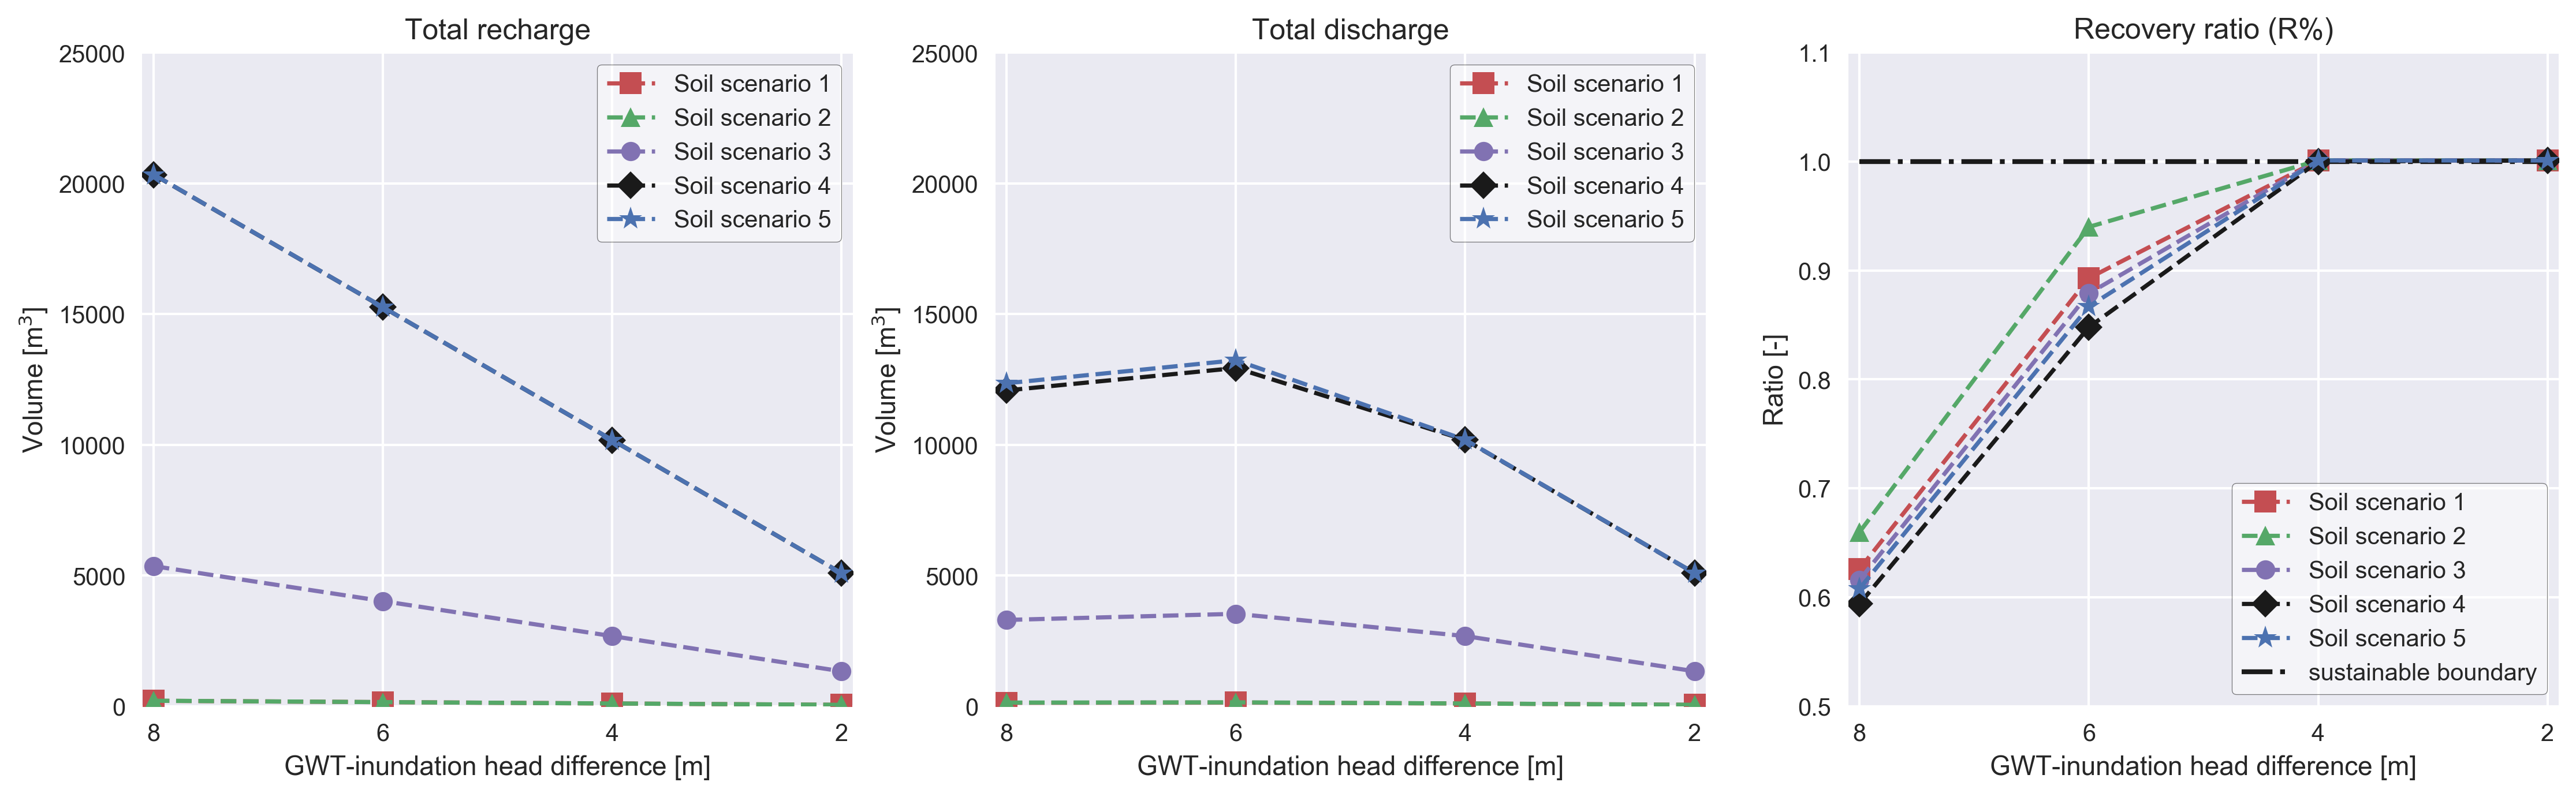
\includegraphics[width=1.0\linewidth]{Results_sens_del_h}
 \captionsetup{justification=centering} 
 \caption{Results of yearly total volumes (in, out, ratio) by reduction of wet season inundation level}
 \label{fig:Results_sens_del_h}
\end{figure}

Note, compared to the base model ($\Delta h$ is 8 m) the total discharge volume is slightly higher for the situation with a $\Delta h$ is 6 m. A system performance that can be justified by the defined initial groundwater table. The higher GWT of latter situation (-5 m instead of -6 m) ensures higher groundwater pressure, causing a (although minor) higher well discharge rate. \\


* Note, although not clearly visible (especially, when total recharge volumes are taken into account) all soil scenarios are included in the presented figures.  \\
%The net elevation of 1 m GWT provides a slightly higher hydraulic gradient.  
 
%when affected by borehole clogging depth.  deSystem cleaning has a positive impact on both the wet season recharge and dry season discharge. Total volumes infiltrated and withdrawn are approximately linear dependent on the (clean) well screen length. Effects of non-uniform flow (partially aguifer penetration) are not of significance for the simulation conditions applied in this study.  
%
%Relatively seen, the discharge is affected more than the recharge, causing the occurance of lower Recovery ratios. 
%
%
%System cleaning ensures a increase in recovery ratios (for all soil scenarios). In an absolute sense the total volumes discharged are slightly more affected by cleaning compared to recharged volumes. In general recovery ratio increase is not significant. Moreover the ratios stay within the range of sustainable use. Deepening the borehole (to its original length) improves system operation. Cleaning of (partially) clogged systems is advisable.

\section{The dimensionless ASR system recharge factor}
\label{section:dim_fac}
The prior research sections (\ref{section:ASR_upscaling} - \ref{section:sens_analysis}) contain an abundance of model modifications. The modifications are related to both the ASR system (\ref{section:ASR_upscaling}) and natural conditions (\ref{section:sens_analysis}). This section tries to expose the relationship between parameters and the ASR system recharge performance. \\

In this process the (recharge) situation of the ASR system is further simplified. The well skin resistance is ignored. As stated by \citet{Bruggeman1999}, the analytical solution of this simplified problem (with constant inundation level) is given by: 

\begin{equation}
\phi (r, t) = h - \frac{2h}{\pi} \int_{0}^{\infty} \frac{1}{u} h(u, r) \exp ( -\frac{u^2 t}{\beta^2 R^2}) du
\label{eq:brug_22302}
\end{equation}

where the "head" function $h(u, r)$ is given by

\begin{equation}
h (u, r) = \frac{J_0(u) Y_0 (\frac{r}{R}u) - Y_0 (u) J_0 (\frac{r}{R}u)}{J_0^2(u) + Y_0^2(u)}
\label{eq:brug_22302headfunc}
\end{equation}

and 

\begin{equation}
\beta^2 = \frac{S}{kD}
\label{eq:brug_22302beta}
\end{equation}

The following boundary conditions are given: \\
$\phi(r, 0) = 0$, \\
$\phi (\infty, t) = 0$, \\
$\phi(R, t) = h$ \\

Derivative of the head function with respect to r:

\begin{equation}
\frac{ \partial h (u, r)}{\partial r} = \frac{- u J_0(u) Y_1(u \frac{r}{R}) + u Y_0(u) J_1(u \frac{r}{R})}{R (J_0^2(u) + Y_0^2(u))}
\label{eq:brug_22302deriv}
\end{equation}

Which means 

\begin{equation}
\frac{\partial \phi (r, t)}{\partial r} = \frac{2h}{\pi} \int_0^{\infty} \frac{1}{u} \frac{\partial h (u, r)}{\partial r} \exp( -\frac{u^2 t}{\beta^2 R^2}) du
\label{eq:brug_22302deriv}
\end{equation}

%The prior research sections (\ref{section:ASR_upscaling} - \ref{section:sens_analysis}) contain an abundance of model modifications. The modifications are related to both the ASR system (\ref{section:ASR_upscaling}) and natural conditions (\ref{section:sens_analysis}). Regardless its origin, this section tries to enclose the ASR system performance in terms of recharge in a single 'dimensionless ASR system recharge factor'. \\
%\bigskip
%\bigskip
%\bigskip
%\bigskip
%\bigskip

\section{Results \& Conclusions}
\label{section:Upscaling_conclusions}
This section contains conclusions on the performance of an ASR system, potentially applicable on northern Ghana conditions. The conclusions on system performance are drawn from the synthetic base model, the simulated ASR system modifications and the system sensitivity analysis. \\

%This section contains the conclusions that can be drawn from the site visits and the analysis of pumping test data. The final part of this section describes how this data was used to derive parameters for scenarios to study potential methods for improvements of ASR systems in northern Ghana.  \\

\textbf{Performance of a synthetic ASR system in northern Ghana}
\begin{itemize}
\item{Recharge \& discharge volumes } \\
The total inflow and outflow volumes are both affected by the magnitude of the transmissivity value. An increase of the transmissivity value, in the range of 1 - 100 (m$^2$/d), results in acquired volumes that are significantly higher. The presence of a well skin resistance (transmissivity dependent) may play a role in this context. The bandwidth variance in storativity values, 1e-3 - 1e-2 (-), appears to have only limited influence on the obtained volumes. The shift in storativity values applied (within bandwidth range), sorts minimal effects on the total inflow volume. While, the discharge volumes are somewhat positively affected by an increased storativity. The (small) storativity bandwidth-scope is insufficient to draw further conclusions. 
\item{Sustainable use} \\
Under the applied conditions of subsurface composition and ASR system use,  recovery ratios (for all soil scenarios) stay within the limits of sustainability. In eight months of daily (4 hours) pump operation, with a discharge bounded by a maximum drawdown ($\Delta$h of 14 m), it is not possible to fully recover the water volumes recharged due to four months of constant inundation ($\Delta h$ is 8 m).
\end{itemize}

\textbf{ASR system improvements}
\begin{itemize}
\item{Preservation of sustainable use} \\
Higher total discharge volumes can be obtained by an extension of the dry season daily pumping time. By considering the predefined conditions (e.g. wet season constant 2 m flooding, dry season daily pumping operation of 4 hour), it is advisable pumping operation should not exceed a 6 till 7 hour daily duration (8 months). Independently from the soil scenario, a sustainable system use can in this way potentially be retained. 
\item{Increase in recharge \& discharge volumes}\\
In terms of volumes (and Recovery ratios), an ASR system can be improved by both the enlargement of the borehole cross-sectional dimension and the reduction of the well skin resistance. Within the research scope ($r_w$ = 0.0635-0.3175 m and $k_{gp}$ = 0.2-1.8*$K_h$), the obtained base model volumes are more than doubled by these types of improvement. A non-linear relation exists between the 'size' of the system improvement and the magnitude of obtained volumes. A significant water profit can be obtained by relative small base model modifications.
\end{itemize}

%Beyond the extents of improvement applied in this research a maximum in obtained water volumes can be expected. 

\textbf{ASR system sensitivity to nature}
\begin{itemize}
\item{Recharge volumes}\\
The relation between the partially penetrating well screen length (research scope: 10 - 30 m) and inflow and outflow is slightly off from linear. When the active screen length reduces (more accumulation of sediment), the essence of cleaning becomes not only in absolute terms but also relatively more important. Within the research time-span, the system recharge volumes are by approximation linear related (positively) to the duration of the constant level flooding (range 1 - 4 months) and the depth of the inundation level. In the latter case, it is more precisely the difference between the flood level and (initial) groundwater table (hydraulic gradient) that is normative ($\Delta$h range 2 - 8 m). 
\end{itemize}

%the partially well penetration length (range 10 - 30 m), When further clogging occurs the relative essence of cleaning becomes more important. 